\documentclass{szablonPG}
\usepackage[style=numeric, language=polish, backend=biber, sorting=nyt, giveninits=true, maxbibnames=4, minbibnames=1, dateabbrev=false, urldate=long]{biblatex}
\usepackage{dirtree}
\usepackage{listing_schemat}
\usepackage{polski}
\usepackage[T1]{fontenc}
\usepackage[utf8]{inputenc}
\usepackage{tikz}
\usetikzlibrary{positioning,fit,arrows.meta,calc}

\addbibresource{references.bib}

\newcommand{\transformerstack}[2]{%
    % Back layer
    \node[
        draw,
        fill=purple!10,
        thick,
        rounded corners=1pt,
        minimum width=2.5cm,
        minimum height=0.8cm,
        #1,
        xshift=0.30cm,
        yshift=0.30cm
    ] (#2back) {};

    % Middle layer
    \node[
        draw,
        fill=purple!15,
        thick,
        rounded corners=1pt,
        minimum width=2.5cm,
        minimum height=0.8cm,
        #1,
        xshift=0.15cm,
        yshift=0.15cm
    ] (#2mid) {};

    % Front layer
    \node[
        draw,
        fill=purple!25,
        thick,
        rounded corners=1pt,
        minimum width=2.5cm,
        minimum height=0.8cm,
        align=center,
        #1
    ] (#2) {Transformer\\Encoder};

    % × N
    \node[
        font=\small\bfseries,
        below=0.25cm of #2
    ] (#2label) {$\times N$};
}

\usepackage{geometry}
\usepackage{titlesec}
\usepackage{graphicx}
\usepackage{setspace}
\usepackage{times}
\usepackage{pdfpages}
\usepackage[normalem]{ulem}
\usepackage{amsmath}
\usepackage{amssymb}
\usepackage{array}
\newcolumntype{L}[1]{>{\raggedright\arraybackslash}p{#1}}
\usepackage{booktabs}
\usepackage{longtable}
\usepackage{csquotes}
\usepackage{microtype}
\usepackage{placeins}
\usepackage{adjustbox}

% Configure URL breaking for bibliography
\setcounter{biburlnumpenalty}{9000}
\setcounter{biburlucpenalty}{9000}
\setcounter{biburllcpenalty}{9000}
\usepackage{xurl}
\appto{\bibsetup}{\emergencystretch=3em}
\DeclareFieldFormat{urldate}{\mkbibparens{dost\k{e}p:\space#1}}


\newcommand{\todo}[1]{\textcolor{red}{TODO: #1}\PackageWarning{TODO:}{#1!}}

% Inicjały autorów przy tytułach rozdziałów (nie zmieniane na wersaliki w spisie treści)
\newcommand{\aut}[1]{\texorpdfstring{\NoCaseChange{ (#1)}}{ (#1)}}

\begin{document}


\includepdf{StronaTytulowa_pl.pdf}
\newpage
\thispagestyle{empty}
\mbox{}
\newpage

\chapter*{Streszczenie}
Niniejsza praca poświęcona jest analizie możliwości współczesnych modeli automatycznego rozpoznawania mowy (ASR) w zakresie uczenia semantycznych reprezentacji danych, zarówno w ujęciu wielojęzycznym, jak i w odniesieniu do słownictwa specjalistycznego. W pierwszym etapie przeanalizowano reprezentacje przestrzeni ukrytej różnych modeli ASR, oceniając stopień, w jakim odzwierciedlają one informacje semantyczne. W tym celu wykorzystano reprezentacje wektorowe transkrypcji uzyskane za pomocą trzech różnych modeli reprezentacji wektorowej (tj. embeddingowych) tekstu. Następnie zaproponowano dwie nowe architektury głębokich sieci neuronowych, wykorzystujące istniejące modele ASR i przeznaczone do multimodalnego wyszukiwania dokumentów na podstawie zapytań w postaci sygnału mowy. W ostatnim etapie wyniki wcześniejszych analiz wykorzystano do opracowania kompleksowego systemu wyszukiwania dokumentów dla specjalistycznych danych medycznych w języku polskim. System ten posłużył następnie do porównania i oceny różnych rozwiązań stosowanych w realizacji tego zadania.
\chapter*{Abstract}
This work investigates the capabilities of contemporary automatic speech recognition (ASR) models to learn semantic representations of data, both in multilingual settings and in the context of specialized vocabulary. First, latent-space representations derived from different ASR models were analyzed to assess the extent to which they capture semantic information. For this purpose, vector representations of the corresponding transcriptions, generated using three different text embedding models, were employed. Next, two novel deep-learning architectures based on existing ASR models were proposed for multimodal document retrieval using spoken queries. Finally, the findings from the preceding analyses were used to develop a comprehensive document retrieval system for specialized Polish medical data. The resulting system was subsequently employed to compare and evaluate different approaches to this task.

\chapter*{Wykaz ważniejszych oznaczeń i skrótów}

\noindent\textbf{Skróty}

\begin{longtable}{@{}p{2.6cm}p{\dimexpr\linewidth-2.6cm-2\tabcolsep\relax}@{}}
ABTT & \textit{All But the Top} -- metoda przetwarzania końcowego embeddingów usuwająca średnią i pierwsze składowe główne \\
APM & \textit{Attention Pool Model} -- proponowany model dopasowania reprezentacji mowy do przestrzeni modelu embeddingowego \\
ASR & automatyczne rozpoznawanie mowy (ang. \textit{Automatic Speech Recognition}) \\
BERT & \textit{Bidirectional Encoder Representations from Transformers} \\
CER & współczynnik błędów znakowych (ang. \textit{Character Error Rate}) \\
CNN & konwolucyjna sieć neuronowa (ang. \textit{Convolutional Neural Network}) \\
EAM & \textit{Embedding Alignment Model} -- proponowany model tworzący wspólną przestrzeń embeddingową mowy i tekstu \\
HMM & ukryty model Markowa (ang. \textit{Hidden Markov Model}) \\
InfoNCE & kontrastowa funkcja straty (ang. \textit{Noise-Contrastive Estimation}) \\
kNN & algorytm $k$-najbliższych sąsiadów (ang. \textit{k-Nearest Neighbours}) \\
LLM & duży model językowy (ang. \textit{Large Language Model}) \\
LoRA & adaptacja niskiego rzędu (ang. \textit{Low-Rank Adaptation}) \\
M4T & model SeamlessM4T (ang. \textit{Massively Multilingual and Multimodal Machine Translation}) \\
MAP & średnia precyzja uśredniona (ang. \textit{Mean Average Precision}) \\
MFCC & współczynniki cepstralne w skali mel (ang. \textit{Mel-Frequency Cepstral Coefficients}) \\
MMD & maksymalna rozbieżność średnich (ang. \textit{Maximum Mean Discrepancy}) \\
MMR & \textit{Maximal Marginal Relevance} -- metoda dywersyfikacji wyników wyszukiwania \\
MRR & średnia odwrotność rangi (ang. \textit{Mean Reciprocal Rank}) \\
NDCG & znormalizowany skumulowany zysk dyskontowany (ang. \textit{Normalized Discounted Cumulative Gain}) \\
PCA & analiza składowych głównych (ang. \textit{Principal Component Analysis}) \\
RAG & generowanie wspomagane wyszukiwaniem (ang. \textit{Retrieval-Augmented Generation}) \\
ROUGE & \textit{Recall-Oriented Understudy for Gisting Evaluation} -- metryka jakości generowanego tekstu \\
RRF & \textit{Reciprocal Rank Fusion} -- metoda łączenia list rankingowych \\
SAE & rzadki autoenkoder (ang. \textit{sparse autoencoder}) \\
SBERT & Sentence-BERT -- model embeddingowy zdań \\
SVCCA & \textit{Singular Vector Canonical Correlation Analysis} -- metoda porównywania reprezentacji \\
TF-IDF & \textit{Term Frequency -- Inverse Document Frequency} \\
TTS & synteza mowy (ang. \textit{Text-to-Speech}) \\
WER & współczynnik błędów słownych (ang. \textit{Word Error Rate}) \\
\end{longtable}

\newpage

\noindent\textbf{Oznaczenia}

\begin{longtable}{@{}p{2.6cm}p{\dimexpr\linewidth-2.6cm-2\tabcolsep\relax}@{}}
$x^a$, $x^p$, $x^n$ & przykład bazowy, pozytywny i negatywny w trójce (ang. \textit{triplet}) \\
$S(x_{emb,asr})$ & różnica podobieństw w trójce między modelem embeddingowym a modelem ASR \\
$\mathrm{MMD}$ & metryka maksymalnej rozbieżności średnich między rozkładami reprezentacji \\
$C$ & metryka poprawnej klasyfikacji relacji semantycznej w trójce \\
$H$ & reprezentacja ukryta enkodera, $H \in \mathbb{R}^{n \times d}$ \\
$M$ & maska atencji, $M \in \{0,1\}^{n \times 1}$ \\
$E$ & macierz embeddingów, $E \in \mathbb{R}^{N \times d}$ \\
$d$, $D$ & wymiar reprezentacji \\
$N$ & liczba próbek \\
$\mu$, $\sigma$ & parametry położenia i skali dopasowanego rozkładu Studenta \\
$\nu$ & liczba stopni swobody rozkładu Studenta \\
$P(\mathrm{neg} > \mathrm{poz})$ & prawdopodobieństwo poprawnego uchwycenia relacji między przykładami w trójce \\
$\mathcal{L}$ & funkcja straty \\
$\tau$ & współczynnik temperatury w funkcji InfoNCE \\
$\lambda$ & współczynnik wagi składnika funkcji straty lub harmonogramu EMA \\
\end{longtable}

\tableofcontents

% --- Wprowadzenie ---
\chapter{Wprowadzenie\aut{K.Ch.}}
\label{sec:wprowadzenie}
% 
% 

Obecne systemy wyszukiwania informacji coraz częściej integrują technologie oparte na uczeniu maszynowym. Technika \textbf{RAG (Retrieval-Augmented Generation)} integruje mechanizmy generatywne z modułami wyszukiwania informacji, umożliwiając modelom językowym \textbf{LLM} dostęp do kontekstowo istotnych danych podczas generacji odpowiedzi. Dzięki temu możliwe jest znaczne zwiększenie precyzji i warygodności uzyskiwanych wyników. 

Kluczowym elementem modułu wyszukiwania jest reprezentacja danych w przestrzeni wektorowej. Zamiast opierać wyszukiwanie na dopasowaniu słów kluczowych, systemy te wykorzystują \textbf{embeddingi} - numeryczne reprezentacje semantyczne tekstu, obrazów lub innych modalności. Umożliwia to porównywanie znaczenia zapytań i dokumentów na poziomie ich ukrytej reprezentacji (latent space representation), co znacząco zwiększa trafność wyników w porównaniu z klasycznymi metodami leksykalnymi.

Jednym z wyzwań stojących przed tego typu systeami jest efektywne łączenie różnych modalności danych, w szczególności sygnału akustycznego (mowy) i tekstu. W większości obecnych rozwiązań proces wyszukiwania informacji na podstawie zapytań głosowych realizowany jest dwuetapowo. Najpierw model \textbf{ASR (Automatic Speech Recognition)} konwertuje sygnał dzwiękowy na tekst. Następnie model embeddingowy przekształca tekst do przestrzeni wektorowej. Choć podejście to jest szeroko stosowane to wprowadza ono dodatkową warstwę pośrednią, która może prowadzić do utraty części informacji semantycznych i prozodycznych zawartych w mowie, a także do propagacji błędów wynikających z niepoprawnej transkrypcji.

Warto zauważyć, że zarówno modele \textbf{ASR}, jak i embeddingowe, wymagają długiego procesu uczenia oraz ogromnych zbiorów danych, co sprawia, że ich ponowne trenowanie lub dostrajanie do nowych zadań jest kosztowne obliczeniowo i czasowo. Dlatego szczególnie istotne staje się opracowanie metod umożliwiających wykorzystanie już istniejących modeli w sposób bardziej zintegrowany.

W odpowiedzi na powyższe ograniczenia możliwe jest wykorzystanie istniejących modeli \textbf{ASR} oraz modeli \textbf{embeddingowych} i opracowanie mechanizmu umożliwiającego mapowanie przestrzeni ukrytej rozpoznanej mowy na przestrzeń ukrytą modelu embeddingowego. Takie rozwiązanie pozwala uniknąć transkrypcji tekstowej, co sprzyja zachowaniu pełniejszej informacji semantycznej i prozodycznej zawartej w sygnale mowy, przy jednoczesnym wykorzystaniu istniejących modeli ASR i embeddingowych.

Celem niniejszej pracy jest opracowanie i analiza systemu umożliwiającego wyszukiwanie informacji w specjalistycznych bazach danych (medycznych) za pomocą zapytań głosowych. W pracy zostanie pretestowana trafność i precyzja wyszukiwania informacji, porównując popularne dwuetapowe podejście z rozwiązaniem wykorzystującym model pośredni - translator ukrytych reprezentacji audio modelu ASR a modelem embeddingowym.
\subsection{Kontekst i motywacja}

\subsubsection{Wyszukiwanie informacji w bazach specjalistycznych}

Tradycyjne systemy wyszukiwania informacji opierały się na modelu boolowskim (ang. \textit{Boolean Information Retrieval}), w którym zapytania formułowane są za pomocą operatorów logicznych AND, OR oraz NOT \cite{salton1983introduction}. Podejście to, choć precyzyjne w założeniach teoretycznych, wymaga od użytkownika znajomości składni zapytań i nie uwzględnia zjawisk językowych takich jak synonimia czy polisemia \cite{manning2008introduction}. Ograniczenia te doprowadziły do rozwoju systemów typu \textit{free text retrieval}, w których zapytania formułowane są w języku naturalnym, a dokumenty rankingowane według stopnia dopasowania \cite{robertson2009probabilistic}.

Ewolucja ta jest szczególnie widoczna w kontekście specjalistycznych baz danych, takich jak PubMed czy MEDLINE, które początkowo opierały się na kontrolowanych słownikach (MeSH - \textit{Medical Subject Headings}) i zapytaniach boolowskich \cite{lu2011pubmed}. Współczesne interfejsy tych systemów oferują jednak wyszukiwanie w języku naturalnym z automatycznym rozszerzaniem zapytań o synonimy i terminy pokrewne, co znacząco obniża barierę wejścia dla użytkowników końcowych - lekarzy i badaczy nieposiadających przygotowania z zakresu informatologii. Dalszy postęp w tej dziedzinie wiąże się z zastosowaniem modeli uczenia głębokiego do reprezentacji semantycznej tekstu oraz architektur typu RAG (ang. \textit{Retrieval-Augmented Generation}), które zostały szczegółowo omówione w rozdziale 2.

\subsubsection{Rola przetwarzania mowy w wyszukiwaniu informacji}

Współczesne modele automatycznego rozpoznawania mowy (ang. \textit{Automatic Speech Recognition}, ASR) umożliwiają formułowanie zapytań do systemów wyszukiwania informacji za pomocą mowy, co jest szczególnie istotne w środowiskach klinicznych, gdzie ręczne wprowadzanie tekstu jest niepraktyczne. Modele takie jak Whisper \cite{whisper}, Wav2Vec 2.0 \cite{baevski2020wav2vec} czy HuBERT \cite{hsu2021hubert} osiągają wysoką jakość transkrypcji dla wielu języków, jednak w podejściu kaskadowym (ASR $\rightarrow$ embedding tekstowy $\rightarrow$ wyszukiwanie) błędy transkrypcji propagują się do kolejnych etapów, obniżając jakość wyników wyszukiwania. Szczegółowy przegląd architektury i możliwości tych modeli przedstawiono w rozdziale 2.

\subsubsection{Ograniczenia modeli dla języka polskiego i domen specjalistycznych}
\label{sec:motywacja}

Współczesne modele uczenia głębokiego są w przeważającej mierze trenowane na danych w języku angielskim. Zbiory danych wykorzystywane do pretrainingu dużych modeli językowych, takie jak Common Crawl, Wikipedia czy arXiv, charakteryzują się znaczącą nadreprezentacją treści anglojęzycznych \cite{joshi2020state}. Szacuje się, że język angielski stanowi ponad 90\% danych treningowych wielu popularnych modeli, mimo że jest językiem ojczystym jedynie dla około 5\% światowej populacji \cite{bender2021dangers}.

Nierównowaga ta ma istotne konsekwencje dla jakości modeli w kontekście języków innych niż angielski. Języki regionalne, w tym język polski, są klasyfikowane jako języki o średnich lub niskich zasobach (ang. \textit{mid-resource} lub \textit{low-resource languages}) \cite{joshi2020state}. Modele wielojęzyczne, takie jak mBERT \cite{devlin2019bert}, XLM-RoBERTa \cite{conneau2020unsupervised} czy Whisper \cite{whisper}, stanowią próbę rozwiązania tego problemu, jednak badania empiryczne wskazują, że ich jakość dla języków innych niż angielski jest systematycznie niższa \cite{wu2020all}, szczególnie w zadaniach wymagających znajomości specjalistycznej terminologii.

Ograniczenia modeli ogólnego przeznaczenia w kontekście domen specjalistycznych wynikają nie tylko z nierównowagi językowej, ale również z charakteru danych treningowych. Modele ASR są trenowane głównie na podcastach, filmach i nagraniach z platformy YouTube \cite{whisper}, które rzadko zawierają specjalistyczną terminologię medyczną. Analogiczny problem dotyczy modeli embeddingowych, których reprezentacje wektorowe terminów specjalistycznych mogą nie odzwierciedlać poprawnie ich znaczenia w kontekście domenowym \cite{lee2020biobert}. Istnieją rozwiązania w postaci modeli dostosowanych do konkretnych domen, jednak dotyczą one przede wszystkim języka angielskiego (zob. rozdział 2).

Kluczowym wyzwaniem pozostaje ograniczona dostępność specjalistycznych zbiorów danych dla języka polskiego. Podczas gdy dla języka angielskiego istnieją obszerne zbiory tekstów medycznych, takie jak MIMIC-III \cite{johnson2016mimic} czy PubMed, dla języka polskiego brakuje porównywalnych zasobów. Dokumentacja medyczna w języku polskim jest rozproszona, często niedostępna ze względów prawnych i wymaga pracochłonnej anonimizacji przed wykorzystaniem do celów badawczych. Sytuacja ta tworzy błędne koło: brak danych uniemożliwia trening wysokiej jakości modeli, co z kolei utrudnia automatyzację procesów, które mogłyby wspomóc tworzenie i przetwarzanie takich zbiorów.

% ----------------------------------------
\subsection{Proponowane podejście}

\subsubsection{System wyszukiwania oparty na transkrypcji audio i wektorowej bazie danych}

Klasyczna architektura systemu wyszukiwania informacji na podstawie zapytań głosowych opiera się na sekwencyjnym przetwarzaniu sygnału audio przez oddzielne moduły. Podejście to można określić jako pipeline kaskadowy, w którym każdy etap przetwarza dane wyjściowe etapu poprzedniego.

W pierwszym etapie sygnał audio jest przetwarzany przez model ASR, taki jak Whisper \cite{whisper} lub jego wersja dostrojona do domeny specjalistycznej. Wynikiem tego etapu jest transkrypcja tekstowa zapytania użytkownika. Następnie tekst jest przekształcany przez model embeddingowy w reprezentację wektorową. Modele takie jak Sentence-BERT \cite{reimers2019sentence} czy Jina Embeddings \cite{gunther2023jina} generują wektor o stałym wymiarze, reprezentujący semantyczną treść zapytania.

Uzyskany wektor zapytania jest porównywany z wektorami dokumentów zindeksowanych w wektorowej bazie danych. Systemy takie jak FAISS \cite{johnson2019billion} czy Milvus \cite{wang2021milvus} umożliwiają efektywne wyszukiwanie przybliżonych najbliższych sąsiadów (ang. \textit{approximate nearest neighbor search}) w przestrzeniach wielowymiarowych. Na podstawie miary podobieństwa system zwraca $k$ dokumentów najbardziej zbliżonych semantycznie do zapytania.

Opcjonalnie architektura może być rozszerzona o komponent generacyjny zgodnie ze wzorcem RAG \cite{lewis2020retrieval}. W takim przypadku wyszukane dokumenty stanowią kontekst dla dużego modelu językowego, który generuje odpowiedź w języku naturalnym, syntetyzując informacje z wielu źródeł. Schemat opisanej architektury przedstawiono na Rysunku \ref{fig:kaskadaArchitecture}.

\begin{figure}[htbp]
    \centering
    \begin{tikzpicture}[
    scale=0.6,
    transform shape,
    font=\small,
    block/.style={
        draw,
        rounded corners=2pt,
        thick,
        minimum width=2.8cm,
        minimum height=1.0cm,
        align=center
    },
    data/.style={block, fill=gray!12},
    model/.style={block, fill=blue!20},
    embm/.style={block, fill=purple!20},
    store/.style={block, fill=orange!25},
    ann/.style={block, fill=yellow!25},
    opt/.style={block, fill=green!15, dashed},
    arrow/.style={-{Stealth[]}, thick},
    optarrow/.style={-{Stealth[]}, thick, dashed},
    phase/.style={draw=gray, dashed, rounded corners=4pt, inner sep=0.3cm}
]

% ============================================================
% FAZA ZAPYTANIA
% ============================================================
\node[data] (audio) {Nagranie\\audio};
\node[model, right=0.7cm of audio] (asr) {Model ASR\\(Whisper)};
\node[data, right=0.7cm of asr] (txt) {Tekst\\transkrypcji};
\node[embm, right=0.7cm of txt] (qemb) {Model\\embeddingowy};
\node[data, right=1.1cm of qemb] (qvec) {Wektor\\zapytania};
\node[ann, right=1.1cm of qvec] (search) {Wyszukiwanie ANN};

\draw[arrow] (audio) -- (asr);
\draw[arrow] (asr) -- (txt);
\draw[arrow] (txt) -- (qemb);
\draw[arrow] (qemb) -- node[below, font=\scriptsize, text=gray] {$1\times d_{\mathrm{emb}}$} (qvec);
\draw[arrow] (qvec) -- (search);

% ============================================================
% FAZA INDEKSOWANIA (równolegle, offline)
% ============================================================
\node[data, above=1.6cm of qemb] (docs) {Dokumenty\\tekstowe};
\node[embm, above=1.6cm of qvec] (demb) {Model\\embeddingowy};
\node[store, above=1.6cm of search] (db) {Wektorowa\\baza danych};

\draw[arrow] (docs) -- (demb);
\draw[arrow] (demb) -- node[below, font=\scriptsize, text=gray] {$1\times d_{\mathrm{emb}}$} (db);
\draw[arrow] (db) -- node[right, font=\scriptsize] {indeks} (search);

% ============================================================
% WYNIKI + OPCJONALNY KOMPONENT GENERACYJNY (RAG)
% ============================================================
\node[data, below=0.9cm of search] (topk) {Top-$k$\\dokumentów};
\node[opt, below=0.9cm of topk] (llm) {LLM\\(generacja)};
\node[opt, below=0.9cm of llm] (ans) {Odpowiedź w\\języku naturalnym};

\draw[arrow] (search) -- (topk);
\draw[optarrow] (topk) -- node[left, font=\scriptsize\itshape] {opcjonalnie (RAG)} (llm);
\draw[optarrow] (llm) -- (ans);

% ============================================================
% RAMKI FAZ
% ============================================================
\node[phase, fit=(docs)(db),
      label={[font=\small\itshape, gray]above:Faza indeksowania (offline)}] {};
\node[phase, fit=(audio)(search),
      label={[font=\small\itshape, gray]above left:Faza zapytania}] {};

\end{tikzpicture}

    \caption{Architektura kaskadowa systemu wyszukiwania informacji na podstawie zapytań głosowych. Faza indeksowania dokumentów przebiega niezależnie od fazy zapytania. Komponent generacyjny (RAG) jest opcjonalnym rozszerzeniem architektury.}
    \label{fig:kaskadaArchitecture}
\end{figure}

Architektura kaskadowa oferuje szereg zalet praktycznych. Transkrypcja tekstowa stanowi dodatkowy produkt przetwarzania, który może być wykorzystany do celów dokumentacyjnych lub archiwalnych. Użytkownik ma możliwość weryfikacji i ewentualnej korekty rozpoznanego tekstu przed wykonaniem wyszukiwania, co zwiększa kontrolę nad procesem. Transparentność systemu ułatwia debugowanie. Każdy etap może być analizowany niezależnie, co pozwala na identyfikację źródła ewentualnych błędów. Ponadto architektura ta wykorzystuje sprawdzone, dostępne komponenty, które mogą być wymieniane niezależnie w miarę postępu technologicznego.

Podejście kaskadowe wiąże się jednak z istotnymi ograniczeniami. Dwuetapowe przetwarzanie wprowadza dodatkową latencję, co może być problematyczne w zastosowaniach wymagających odpowiedzi w czasie rzeczywistym. Błędy popełnione na etapie transkrypcji propagują się do kolejnych etapów. Niepoprawnie rozpoznany termin specjalistyczny skutkuje generacją błędnego osadzenia (ang. embedding), a w konsekwencji nieadekwatnymi wynikami wyszukiwania. 
W tym miejscu autorzy niniejszej pracy chcieliby się odnieść się do pojęcia embedding, tj. osadzenie, reprezentacja wektorowa, ale też osadzenie słów czy wektoryzacja tekstu w zależności od kontekstu, w którym się to pojęcie pojawia. Warto również zauważyć, że termin ten został spolszczony (embedding) i obecnie jest wykorzystywany w pracach związanych ze sztuczną inteligencją. Dlatgeo autorzy przyjęli, że taka właśnie forma zostanie wykorzystana w opisie prowadzonych eksperymentów.  

Ponadto redukcja sygnału audio do tekstu prowadzi do utraty informacji. Cechy prozodyczne, takie jak intonacja, tempo mowy czy wahania, mogą nieść informację o pewności lub intencji mówiącego. Informacje te są tracone w procesie transkrypcji. Przykładowo, termin medyczny wymówiony z wahaniem może wskazywać na niepewność diagnostyczną, jednak po transkrypcji jest nieodróżnialny od tego samego terminu wymówionego z pewnością.

\subsubsection{Proponowany system wyszukiwania informacji oparty na reprezentacji cech ukrytych modelu ASR}

Alternatywnym podejściem jest bezpośrednie wykorzystanie reprezentacji ukrytych generowanych przez enkoder modelu ASR do wyszukiwania informacji, z pominięciem etapu transkrypcji tekstowej. Koncepcja ta, określana jako Speech-to-Retrieval, opiera się na założeniu, że reprezentacje ukryte modeli ASR zawierają informację semantyczną wystarczającą do realizacji zadań wyszukiwania.

Modele takie jak Wav2Vec 2.0 \cite{baevski2020wav2vec}, HuBERT \cite{hsu2021hubert} czy enkoder modelu Whisper generują w warstwach pośrednich reprezentacje wektorowe segmentów audio. Reprezentacje te, będące wynikiem przetwarzania przez głębokie sieci neuronowe, kodują informację na różnych poziomach abstrakcji. Warstwy bliższe wejściu reprezentują cechy akustyczne niskiego poziomu, podczas gdy warstwy głębsze mogą kodować informację fonologiczną, leksykalną, a potencjalnie również semantyczną \cite{pasad2021layer}.

Architektura proponowanego systemu składa się z enkodera ASR, warstwy projekcji oraz wektorowej bazy danych. Sygnał audio jest przetwarzany przez enkoder, który generuje sekwencję reprezentacji ukrytych. Sekwencja ta jest następnie agregowana (np. przez uśrednienie lub mechanizm uwagi) i przekształcana przez warstwę projekcji do przestrzeni wektorowej zgodnej z embeddingami tekstowymi dokumentów. Uzyskany wektor służy do wyszukiwania w bazie wektorowej analogicznie jak w architekturze kaskadowej. Schemat proponowanej architektury przedstawiono na Rysunku \ref{fig:s2rArchitecture}.

\begin{figure}[htbp]
    \centering
    \begin{tikzpicture}[
    scale=0.55,
    transform shape,
    font=\small,
    block/.style={
        draw,
        rounded corners=2pt,
        thick,
        minimum width=2.6cm,
        minimum height=1.0cm,
        align=center
    },
    data/.style={block, fill=gray!12},
    model/.style={block, fill=blue!20},
    embm/.style={block, fill=purple!20},
    adapt/.style={block, fill=teal!25},
    store/.style={block, fill=orange!25},
    ann/.style={block, fill=yellow!25},
    opt/.style={block, fill=green!15, dashed},
    arrow/.style={-{Stealth[]}, thick},
    optarrow/.style={-{Stealth[]}, thick, dashed},
    phase/.style={draw=gray, dashed, rounded corners=4pt, inner sep=0.4cm}
]

% ============================================================
% FAZA ZAPYTANIA (bez etapu transkrypcji)
% ============================================================
\node[data] (audio) {Nagranie\\audio};
\node[model, right=0.9cm of audio] (enc) {Enkoder ASR};
\node[data, right=1.5cm of enc] (latent) {Reprezentacja\\ukryta};
\node[model, right=0.9cm of latent] (agg) {Agregacja\\sekwencji};
\node[adapt, right=1.5cm of agg] (proj) {Warstwa projekcji\\(adapter)};
\node[data, right=1.9cm of proj] (qvec) {Wektor\\zapytania};
\node[ann, right=1.9cm of qvec] (search) {Wyszukiwanie ANN};

\draw[arrow] (audio) -- (enc);
\draw[arrow] (enc) -- node[above, font=\scriptsize] {$h_{1..T}$}
    node[below, font=\scriptsize, text=gray] {$T\times d$} (latent);
\draw[arrow] (latent) -- (agg);
\draw[arrow] (agg) -- node[above, font=\scriptsize] {$\bar{h}$}
    node[below, font=\scriptsize, text=gray] {$1\times d$} (proj);
\draw[arrow] (proj) -- node[below, font=\scriptsize, text=gray] {$1\times d_{\mathrm{emb}}$} (qvec);
\draw[arrow] (qvec) -- (search);

% ============================================================
% FAZA INDEKSOWANIA (dokumenty nadal indeksowane tekstowo)
% ============================================================
\node[data, above=2.6cm of proj] (docs) {Dokumenty\\tekstowe};
\node[embm, above=2.6cm of qvec] (demb) {Model\\embeddingowy};
\node[store, above=2.6cm of search] (db) {Wektorowa\\baza danych};

\draw[arrow] (docs) -- (demb);
\draw[arrow] (demb) -- node[below, font=\scriptsize, text=gray] {$1\times d_{\mathrm{emb}}$} (db);
\draw[arrow] (db) -- node[right, font=\scriptsize] {indeks} (search);

% wspólna przestrzeń wektorowa: cel treningu adaptera
\draw[{Stealth[]}-{Stealth[]}, dotted, thick, gray]
    (demb.south) -- node[left, font=\scriptsize\itshape, text=gray]
    {wspólna przestrzeń} (qvec.north);

% ============================================================
% WYNIKI + OPCJONALNY KOMPONENT GENERACYJNY (RAG)
% ============================================================
\node[data, below=1.2cm of search] (topk) {Top-$k$\\dokumentów};
\node[opt, below=1.2cm of topk] (llm) {LLM\\(generacja)};
\node[opt, below=1.2cm of llm] (ans) {Odpowiedź w\\języku naturalnym};

\draw[arrow] (search) -- (topk);
\draw[optarrow] (topk) -- node[left, font=\scriptsize\itshape] {opcjonalnie (RAG)} (llm);
\draw[optarrow] (llm) -- (ans);

% ============================================================
% RAMKI FAZ
% ============================================================
\node[phase, fit=(docs)(db),
      label={[font=\small\itshape, gray]above:Faza indeksowania (offline)}] {};
\node[phase, fit=(audio)(search),
      label={[font=\small\itshape, gray]above left:Faza zapytania (bez transkrypcji)}] {};

\end{tikzpicture}

    \caption{Architektura systemu wyszukiwania opartego na reprezentacji cech ukrytych modelu ASR (\textit{Speech-to-Retrieval}). Etap transkrypcji tekstowej zostaje pominięty, a warstwa projekcji odwzorowuje reprezentację audio do przestrzeni wektorowej modelu embeddingowego, w której zindeksowane są dokumenty tekstowe.}
    \label{fig:s2rArchitecture}
\end{figure}

Kluczowymi elementami architektury są agregacja sekwencji oraz warstwa projekcji (adapter). Zadaniem agregacji jest wydobycie najistotniejszych informacji z sekwencji reprezentacji ukrytych i sprowadzenie jej do pojedynczego wektora, czyli spłaszczenie reprezentacji o wymiar czasu ($T \times d \rightarrow 1 \times d$). Warstwa projekcji odwzorowuje następnie tak uzyskaną reprezentację z przestrzeni enkodera ASR do przestrzeni embeddingów tekstowych. Trening tych komponentów wymaga zbioru par (audio, tekst) wraz z odpowiadającymi im embeddingami tekstowymi. Celem optymalizacji jest minimalizacja odległości między projekcją reprezentacji audio a embeddingiem odpowiadającego tekstu.

Potencjalne zalety proponowanego podejścia obejmują redukcję latencji poprzez eliminację etapu dekodowania tekstu oraz możliwość wykorzystania informacji akustycznej niedostępnej w transkrypcji. Ponadto architektura end-to-end otwiera możliwość wspólnej optymalizacji komponentów retrieval i ASR, co może prowadzić do lepszego dostosowania reprezentacji do zadania wyszukiwania.

Podejście to wiąże się jednak z istotnymi wyzwaniami. Brak transkrypcji utrudnia weryfikację i interpretację działania systemu przez użytkownika. Wyjaśnialność systemu jest ograniczona, ponieważ trudniej jest zrozumieć, dlaczego system zwrócił określone dokumenty. Trening warstwy projekcji wymaga odpowiednio dużego zbioru danych. Ponadto modele ASR nie były pierwotnie trenowane z myślą o zadaniach wyszukiwania informacji, co może ograniczać jakość reprezentacji semantycznych.

\subsubsection{Pytania badawcze}

Porównanie przedstawionych architektur prowadzi do sformułowania pytań badawczych stanowiących przedmiot niniejszej pracy:

\begin{enumerate}
    \item Czy reprezentacje ukryte generowane przez modele ASR zawierają wystarczającą informację semantyczną do realizacji zadań wyszukiwania informacji?
    \item Jak jakość wyszukiwania opartego na reprezentacjach ukrytych wypada w porównaniu z podejściem kaskadowym (ASR → embedding tekstowy)?
    \item Jaki wpływ na jakość obu podejść ma język zapytania (polski vs. angielski) oraz domena (terminologia medyczna vs. język ogólny)?
    \item Które warstwy modeli ASR generują reprezentacje najbardziej przydatne do zadań wyszukiwania semantycznego?
\end{enumerate}

Odpowiedzi na te pytania pozwolą na ocenę praktycznej przydatności podejścia Speech-to-Retrieval w kontekście specjalistycznych systemów wyszukiwania informacji dla języka polskiego.

% ----------------------------------------
\subsection{Struktura pracy}

Dalsza część pracy jest zorganizowana w następujący sposób. Rozdział 2 zawiera przegląd literatury obejmujący systemy wyszukiwania informacji, modele embeddingowe,
architekturę RAG oraz współczesne modele ASR. W rozdziale 3 przedstawiono badania nad semantycznością reprezentacji wektorów cech modeli ASR.
Rozdział 4 opisuje ewaluację architektur dopasowania reprezentacji latentnych modeli ASR i modeli embeddingowych. 
Rozdział 5 dzieli się na dwie części. Pierwsza przedstawia system ewaluacji zbudowany na potrzeby pracy. Druga zawiera eksperymenty porównujące architekturę kaskadową
z proponowanym dopasowaniem reprezentacji latentnych oraz omówienie uzyskanych wyników.
Rozdział 6 zawiera podsumowanie i wnioski.


% --- Przegląd ---
\chapter{Przegląd\aut{K.Ch.}}
\label{sec:przeglad}
\section{Systemy wyszukiwania informacji}

\subsection{Ewolucja od wyszukiwania boolowskiego do semantycznego}

Tradycyjne systemy wyszukiwania informacji opierały się na modelu boolowskim, w którym wynik wyszukiwania ma charakter binarny, bez uwzględnienia stopnia dopasowania dokumentu do intencji użytkownika. Rozwój systemów typu \textit{free text retrieval} wprowadził miary takie jak TF-IDF (ang. \textit{Term Frequency-Inverse Document Frequency}), umożliwiające kwantyfikację istotności terminów w kontekście kolekcji dokumentów \cite{sparckjones1972statistical, salton1988term}. Współczynnik TF-IDF przypisuje wyższą wagę terminom występującym często w danym dokumencie, ale rzadko w całej kolekcji, co pozwala na identyfikację słów kluczowych charakterystycznych dla treści dokumentu.

Klasyczne metody reprezentacji tekstu, takie jak model \textit{Bag of Words} (BoW) czy TF-IDF, traktują jednak dokument jako nieuporządkowany zbiór słów, ignorując ich kolejność oraz zależności kontekstowe \cite{harris1954distributional}. Podejście to, określane jako reprezentacja leksykalna, nie uwzględnia podobieństwa semantycznego między wyrażeniami -- terminy ,,zawał serca'' i ,,myocardial infarction'' są traktowane jako całkowicie odrębne jednostki, mimo identycznego znaczenia.

\subsection{Modele embeddingowe}

Przełomem w kierunku reprezentacji semantycznej było wprowadzenie modelu Word2Vec \cite{mikolov2013efficient, mikolov2013distributed}, który mapuje słowa do gęstej przestrzeni wektorowej o niższym wymiarze (typowo 100--300 wymiarów). W przestrzeni tej słowa o podobnym znaczeniu lub występujące w podobnych kontekstach są reprezentowane przez wektory bliskie sobie według miary odległości, takiej jak podobieństwo kosinusowe. Model Word2Vec opiera się na hipotezie dystrybucyjnej Harrisa \cite{harris1954distributional}, zgodnie z którą znaczenie słowa jest determinowane przez kontekst jego występowania.

Ograniczeniem modelu Word2Vec jest generowanie statycznych embeddingów -- każde słowo posiada pojedynczą reprezentację wektorową niezależnie od kontekstu użycia. Problem ten rozwiązują kontekstowe modele językowe oparte na architekturze Transformer \cite{vaswani2017attention}. Model BERT (ang. \textit{Bidirectional Encoder Representations from Transformers}) \cite{devlin2019bert} generuje reprezentacje słów uwzględniające dwukierunkowy kontekst całego zdania, co pozwala na rozróżnienie znaczeń polisemicznych. Adaptacja modelu BERT do zadania generowania embeddingów zdaniowych zaowocowała powstaniem architektury Sentence-BERT \cite{reimers2019sentence}, umożliwiającej efektywne porównywanie podobieństwa semantycznego całych sekwencji tekstowych.

Współczesne badania zmierzają w kierunku multimodalnych przestrzeni embeddingowych, łączących reprezentacje różnych typów danych. Model CLIP \cite{radford2021learning} tworzy wspólną przestrzeń wektorową dla tekstu i obrazów, umożliwiając wyszukiwanie obrazów na podstawie zapytań tekstowych i odwrotnie. Podobne podejście reprezentują modele takie jak ALIGN \cite{jia2021scaling} czy współczesne architektury embeddingowe, takie jak Jina Embeddings \cite{gunther2023jina}, oferujące zunifikowaną przestrzeń dla wielu modalności i języków.

Embedding definiowany jest formalnie jako funkcja $f: \mathcal{X} \rightarrow \mathbb{R}^d$, która mapuje obiekty ze zbioru wejściowego $\mathcal{X}$ (słowa, zdania, dokumenty, obrazy) do $d$-wymiarowej przestrzeni wektorowej, przy czym podobieństwo semantyczne obiektów jest zachowane jako bliskość geometryczna ich reprezentacji wektorowych. Miarą podobieństwa najczęściej stosowaną w praktyce jest podobieństwo kosinusowe:
\begin{equation}
    \text{sim}(\mathbf{u}, \mathbf{v}) = \frac{\mathbf{u} \cdot \mathbf{v}}{\|\mathbf{u}\| \|\mathbf{v}\|}
\end{equation}
gdzie $\mathbf{u}$ i $\mathbf{v}$ są wektorami embeddingów porównywanych obiektów.

\subsection{Architektura RAG}

Duże modele językowe (ang. \textit{Large Language Models}, LLM), takie jak GPT \cite{brown2020language} czy LLaMA \cite{touvron2023llama}, pomimo imponujących zdolności generacyjnych, charakteryzują się istotnymi ograniczeniami w kontekście zastosowań specjalistycznych. Wiedza tych modeli jest zamrożona w momencie zakończenia treningu, co uniemożliwia uwzględnienie informacji aktualnych lub wysoce specjalistycznych. Ponadto modele te są podatne na zjawisko halucynacji -- generowania treści brzmiących wiarygodnie, lecz niezgodnych z faktami \cite{ji2023survey}.

Architektura RAG (ang. \textit{Retrieval-Augmented Generation}) \cite{lewis2020retrieval} stanowi rozwiązanie tych problemów poprzez integrację komponentu wyszukiwania informacji z modelem generacyjnym. System RAG składa się z trzech głównych faz: indeksowania, wyszukiwania oraz generacji. Schemat architektury przedstawiono na Rysunku \ref{fig:ragArchitecture}.

W fazie indeksowania dokumenty źródłowe są przetwarzane i dzielone na fragmenty (ang. \textit{chunks}) o określonej długości. Każdy fragment jest następnie przekształcany przez model embeddingowy w reprezentację wektorową i zapisywany w wektorowej bazie danych wraz z metadanymi umożliwiającymi identyfikację źródła \cite{johnson2019billion}.

Faza wyszukiwania inicjowana jest przez zapytanie użytkownika, które jest transformowane do tej samej przestrzeni wektorowej co zindeksowane dokumenty. Na podstawie miary podobieństwa (typowo podobieństwa kosinusowego lub odległości euklidesowej) system identyfikuje $k$ najbardziej podobnych fragmentów dokumentów.

W fazie generacji model językowy otrzymuje kontekst składający się z wyszukanych fragmentów dokumentów oraz oryginalnego zapytania użytkownika. Na tej podstawie generuje odpowiedź, która może być weryfikowana przez użytkownika poprzez porównanie z dostarczonymi źródłami.

Architektura RAG oferuje szereg zalet w kontekście zastosowań specjalistycznych. Po pierwsze, umożliwia aktualizację bazy wiedzy bez konieczności ponownego trenowania modelu językowego -- wystarczy dodanie nowych dokumentów do indeksu wektorowego. Po drugie, zapewnia wyjaśnialność poprzez możliwość wskazania konkretnych fragmentów dokumentów wykorzystanych do wygenerowania odpowiedzi. Po trzecie, redukuje ryzyko halucynacji poprzez zakotwiczenie generowanej treści w dostarczonym kontekście \cite{shuster2021retrieval}.

\begin{figure}[htbp]
    \centering
    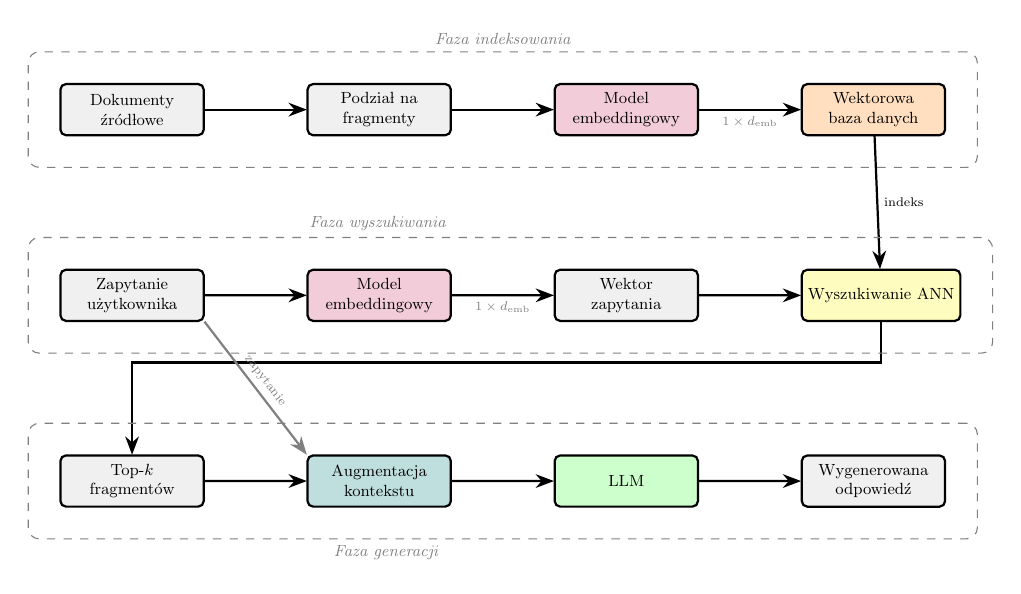
\begin{tikzpicture}[
    scale=0.65,
    transform shape,
    font=\small,
    block/.style={
        draw,
        rounded corners=2pt,
        thick,
        minimum width=2.8cm,
        minimum height=1.0cm,
        align=center
    },
    data/.style={block, fill=gray!12},
    embm/.style={block, fill=purple!20},
    store/.style={block, fill=orange!25},
    ann/.style={block, fill=yellow!25},
    gen/.style={block, fill=green!20},
    ctx/.style={block, fill=teal!25},
    arrow/.style={-{Stealth[]}, thick},
    phase/.style={draw=gray, dashed, rounded corners=4pt, inner sep=0.4cm}
]

% ============================================================
% FAZA INDEKSOWANIA
% ============================================================
\node[data] (docs) {Dokumenty\\źródłowe};
\node[data, right=2.0cm of docs] (chunks) {Podział na\\fragmenty};
\node[embm, right=2.0cm of chunks] (demb) {Model\\embeddingowy};
\node[store, right=2.0cm of demb] (db) {Wektorowa\\baza danych};

\draw[arrow] (docs) -- (chunks);
\draw[arrow] (chunks) -- (demb);
\draw[arrow] (demb) -- node[below, font=\scriptsize, text=gray] {$1\times d_{\mathrm{emb}}$} (db);

% ============================================================
% FAZA WYSZUKIWANIA
% ============================================================
\node[data, below=2.6cm of docs] (query) {Zapytanie\\użytkownika};
\node[embm, right=2.0cm of query] (qemb) {Model\\embeddingowy};
\node[data, right=2.0cm of qemb] (qvec) {Wektor\\zapytania};
\node[ann, right=2.0cm of qvec] (search) {Wyszukiwanie ANN};

\draw[arrow] (query) -- (qemb);
\draw[arrow] (qemb) -- node[below, font=\scriptsize, text=gray] {$1\times d_{\mathrm{emb}}$} (qvec);
\draw[arrow] (qvec) -- (search);
\draw[arrow] (db) -- node[right, font=\scriptsize] {indeks} (search);

% ============================================================
% FAZA GENERACJI
% ============================================================
\node[data, below=2.6cm of query] (topk) {Top-$k$\\fragmentów};
\node[ctx, right=2.0cm of topk] (aug) {Augmentacja\\kontekstu};
\node[gen, right=2.0cm of aug] (llm) {LLM};
\node[data, right=2.0cm of llm] (ans) {Wygenerowana\\odpowiedź};

\draw[arrow] (search.south) -- ++(0,-0.8) -| (topk.north);
\draw[arrow] (topk) -- (aug);
\draw[arrow] (aug) -- (llm);
\draw[arrow] (llm) -- (ans);

% zapytanie użytkownika trafia również do kontekstu promptu
\draw[arrow, gray] (query.south east) -- node[sloped, above, font=\scriptsize, text=gray] {zapytanie} (aug.north west);

% ============================================================
% RAMKI FAZ
% ============================================================
\node[phase, fit=(docs)(db),
      label={[font=\small\itshape, gray]above:Faza indeksowania}] {};
\node[phase, fit=(query)(search),
      label={[font=\small\itshape, gray]above left:Faza wyszukiwania}] {};
\node[phase, fit=(topk)(ans),
      label={[font=\small\itshape, gray]below left:Faza generacji}] {};

\end{tikzpicture}

    \caption{Architektura RAG (\textit{Retrieval-Augmented Generation}) z podziałem na fazy indeksowania, wyszukiwania i generacji. Zapytanie użytkownika trafia zarówno do modelu embeddingowego, jak i -- wraz z wyszukanymi fragmentami -- do kontekstu modelu językowego.}
    \label{fig:ragArchitecture}
\end{figure}


% ---------------------------------------------------
\section{Modele automatycznego rozpoznawania mowy}
\label{sec:modeleASR}

\subsection{Historia i rozwój modeli ASR}

Automatyczne rozpoznawanie mowy (ang. \textit{Automatic Speech Recognition}, ASR) stanowi jedno z klasycznych zagadnień przetwarzania języka naturalnego, którego historia sięga lat siedemdziesiątych XX wieku. Wczesne systemy ASR opierały się na ukrytych modelach Markowa (ang. \textit{Hidden Markov Models}, HMM), które modelowały sygnał mowy jako sekwencję dyskretnych stanów akustycznych \cite{rabiner1989tutorial}. W podejściu tym zakłada się, że obserwowany sygnał akustyczny jest generowany przez ukryty proces stochastyczny, którego stany odpowiadają jednostkom fonetycznym.

Rozszerzeniem modeli HMM były systemy hybrydowe GMM-HMM, łączące ukryte modele Markowa z mieszaninami gaussowskimi (ang. \textit{Gaussian Mixture Models}) \cite{gales2008application}. Mieszaniny gaussowskie służyły do modelowania rozkładu prawdopodobieństwa emisji w poszczególnych stanach HMM, co pozwalało na lepsze uchwycenie zmienności akustycznej sygnału mowy. Systemy te wymagały jednak znacznej wiedzy eksperckiej. Konieczne było ręczne projektowanie cech akustycznych (np. współczynników MFCC), tworzenie słowników wymowy oraz definiowanie modeli fonologicznych dla danego języka.

Przełom w dziedzinie ASR nastąpił wraz z zastosowaniem głębokich sieci neuronowych. Początkowo sieci te zastępowały komponent GMM w systemach hybrydowych DNN-HMM \cite{hinton2012deep}, zachowując strukturę modelowania sekwencji opartą na HMM. Wprowadzenie mechanizmu uwagi (ang. \textit{attention mechanism}) \cite{bahdanau2014neural} oraz architektur typu sekwencja-do-sekwencji (ang. \textit{sequence-to-sequence}) \cite{sutskever2014sequence} umożliwiło bezpośrednie modelowanie zależności między sekwencją akustyczną a sekwencją tekstową bez konieczności jawnego definiowania wyrównania czasowego.

Architektura Transformer \cite{vaswani2017attention}, oparta wyłącznie na mechanizmie uwagi bez komponentów rekurencyjnych, znalazła szerokie zastosowanie w modelach ASR nowej generacji. Modele te, określane jako end-to-end, eliminują tradycyjny pipeline przetwarzania składający się z oddzielnych modułów akustycznego, leksykalnego i językowego. Zamiast tego realizują bezpośrednie mapowanie surowego sygnału audio na sekwencję tekstową, co upraszcza architekturę systemu i eliminuje propagację błędów między modułami.

\subsection{Architektura współczesnych modeli ASR}

Współczesne modele ASR można podzielić na dwie główne kategorie ze względu na metodę treningu: modele wykorzystujące uczenie samonadzorowane (ang. \textit{self-supervised learning}) oraz modele trenowane w sposób nadzorowany (ang. \textit{supervised learning}) na dużych zbiorach transkrybowanych nagrań.

\subsubsection{Wav2Vec 2.0}

Model Wav2Vec 2.0 \cite{baevski2020wav2vec} reprezentuje podejście oparte na uczeniu samonadzorowanym. Architektura składa się z trzech głównych komponentów: enkodera konwolucyjnego (ang. \textit{Convolutional Neural Network}, CNN), transformera oraz modułu kwantyzacji. Enkoder konwolucyjny przetwarza surowy sygnał audio (próbkowany typowo z częstotliwością 16 kHz) i przekształca go w sekwencję wektorów cech o niższej rozdzielczości czasowej. Następnie transformer przetwarza tę sekwencję, generując kontekstowe reprezentacje uwzględniające zależności długozasięgowe. Schemat architektury przedstawiono na Rysunku \ref{fig:wav2vecArchitecture}.

Proces uczenia samonadzorowanego w modelu Wav2Vec 2.0 opiera się na maskowaniu fragmentów sekwencji wejściowej oraz uczeniu kontrastywnym (ang. \textit{contrastive learning}). Model jest trenowany do identyfikacji prawidłowych kwantyzowanych reprezentacji zamaskowanych segmentów ze zbioru negatywnych przykładów. Podejście to pozwala na wykorzystanie ogromnych ilości nieetykietowanych nagrań audio do uczenia semantycznie bogatych reprezentacji akustycznych, bez konieczności korzystania z dużych ilości transkrybowanych nagrań.

Adaptacja modelu do zadania transkrypcji wymaga etapu dostrajania (ang. \textit{fine-tuning}) z wykorzystaniem stosunkowo niewielkiego zbioru danych etykietowanych. Eksperymenty wykazały, że model Wav2Vec 2.0 osiąga konkurencyjne wyniki przy użyciu zaledwie kilkudziesięciu minut transkrybowanych nagrań \cite{baevski2020wav2vec}. Stanowi to istotną zaletę w kontekście języków i domen o ograniczonych zasobach etykietowanych. Dzięki temu podejściu Wav2Vec 2.0 znacząco zredukował zapotrzebowanie na dane z etykietami, jednocześnie poprawiając jakość rozpoznawania mowy w warunkach szumu, zmienności mówców i zróżnicowanego otoczenia akustycznego.

\begin{figure}[htbp]
    \centering
    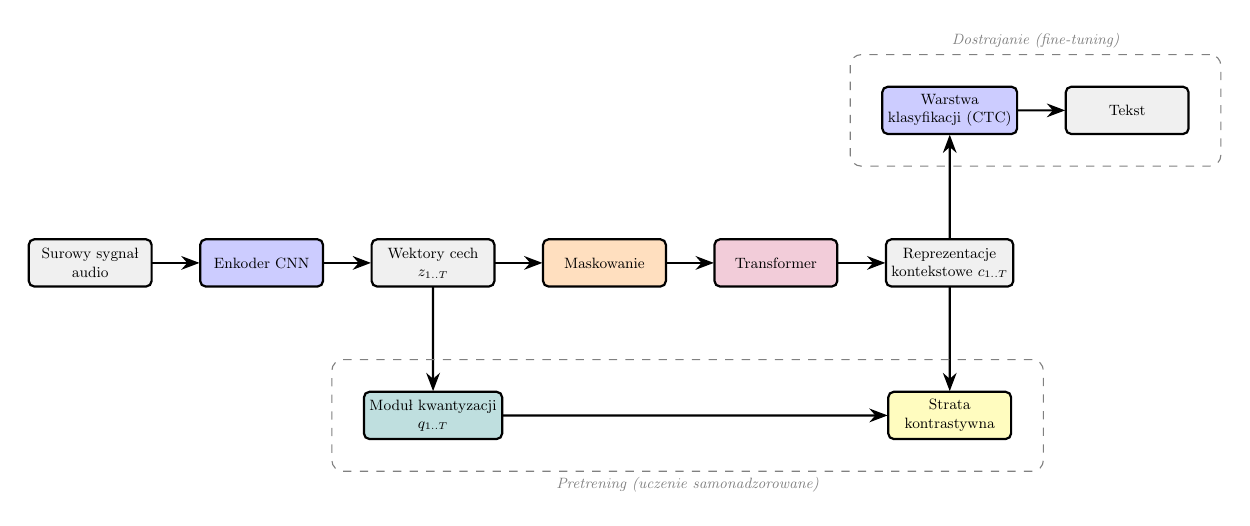
\begin{tikzpicture}[
    scale=0.6,
    transform shape,
    font=\small,
    block/.style={
        draw,
        rounded corners=2pt,
        thick,
        minimum width=2.6cm,
        minimum height=1.0cm,
        align=center
    },
    data/.style={block, fill=gray!12},
    model/.style={block, fill=blue!20},
    trans/.style={block, fill=purple!20},
    op/.style={block, fill=orange!25},
    quant/.style={block, fill=teal!25},
    loss/.style={block, fill=yellow!25},
    arrow/.style={-{Stealth[]}, thick},
    phase/.style={draw=gray, dashed, rounded corners=4pt, inner sep=0.4cm}
]

% ============================================================
% GŁÓWNY PRZEPŁYW
% ============================================================
\node[data] (audio) {Surowy sygnał\\audio};
\node[model, right=1.0cm of audio] (cnn) {Enkoder CNN};
\node[data, right=1.0cm of cnn] (z) {Wektory cech\\$z_{1..T}$};
\node[op, right=1.0cm of z] (mask) {Maskowanie};
\node[trans, right=1.0cm of mask] (tr) {Transformer};
\node[data, right=1.0cm of tr] (c) {Reprezentacje\\kontekstowe $c_{1..T}$};

\draw[arrow] (audio) -- (cnn);
\draw[arrow] (cnn) -- (z);
\draw[arrow] (z) -- (mask);
\draw[arrow] (mask) -- (tr);
\draw[arrow] (tr) -- (c);

% ============================================================
% PRETRENING: kwantyzacja + zadanie kontrastywne
% ============================================================
\node[quant, below=2.2cm of z] (q) {Moduł kwantyzacji\\$q_{1..T}$};
\node[loss, below=2.2cm of c] (contrast) {Strata\\kontrastywna};

\draw[arrow] (z) -- (q);
\draw[arrow] (q) -- (contrast);
\draw[arrow] (c) -- (contrast);

% ============================================================
% DOSTRAJANIE: głowica klasyfikacji
% ============================================================
\node[model, above=2.2cm of c] (head) {Warstwa\\klasyfikacji (CTC)};
\node[data, right=1.0cm of head] (text) {Tekst};

\draw[arrow] (c) -- (head);
\draw[arrow] (head) -- (text);

% ============================================================
% RAMKI FAZ
% ============================================================
\node[phase, fit=(q)(contrast),
      label={[font=\small\itshape, gray]below:Pretrening (uczenie samonadzorowane)}] {};
\node[phase, fit=(head)(text),
      label={[font=\small\itshape, gray]above:Dostrajanie (\textit{fine-tuning})}] {};

\end{tikzpicture}

    \caption{Architektura modelu Wav2Vec 2.0. Podczas pretreningu zamaskowane reprezentacje kontekstowe są porównywane z kwantyzowanymi reprezentacjami cech w ramach zadania kontrastywnego. Etap dostrajania dodaje warstwę klasyfikacji generującą transkrypcję.}
    \label{fig:wav2vecArchitecture}
\end{figure}

\subsubsection{HuBERT}

Model HuBERT (ang. \textit{Hidden-Unit BERT}) \cite{hsu2021hubert} stanowi rozwinięcie koncepcji uczenia samonadzorowanego dla reprezentacji mowy. Podobnie jak Wav2Vec 2.0, HuBERT wykorzystuje architekturę składającą się z enkodera konwolucyjnego oraz transformera. Zasadnicza różnica dotyczy jednak metody uczenia.

W modelu Wav2Vec 2.0 uczenie opiera się na zadaniu kontrastywnym, w którym model rozróżnia prawdziwe reprezentacje zamaskowanych segmentów od negatywnych przykładów. HuBERT natomiast wykorzystuje podejście inspirowane modelem BERT \cite{devlin2019bert} z dziedziny przetwarzania języka naturalnego. Model jest trenowany do przewidywania dyskretnych pseudoetykiet przypisanych zamaskowanym fragmentom sygnału audio. Schemat architektury przedstawiono na Rysunku \ref{fig:hubertArchitecture}.

Pseudoetykiety generowane są w procesie iteracyjnym. W pierwszej iteracji stosuje się algorytm k-średnich (ang. \textit{k-means clustering}) do cech MFCC surowego sygnału audio, uzyskując początkowy zbiór klastrów. Model HuBERT jest następnie trenowany do przewidywania przypisań klastrowych dla zamaskowanych segmentów. W kolejnych iteracjach pseudoetykiety są aktualizowane poprzez zastosowanie algorytmu k-średnich do reprezentacji cech ukrytych wytrenowanego modelu, co prowadzi do coraz bardziej semantycznych grupowań.

Zaletą tego podejścia jest możliwość uczenia bez konieczności definiowania negatywnych przykładów, co upraszcza proces treningowy. Ponadto iteracyjne doskonalenie pseudoetykiet pozwala modelowi na stopniowe odkrywanie struktury językowej sygnału mowy. Eksperymenty wykazały, że HuBERT osiąga wyniki porównywalne lub lepsze od Wav2Vec 2.0 w zadaniach rozpoznawania mowy, szczególnie w scenariuszach z ograniczoną ilością danych etykietowanych \cite{hsu2021hubert}.

Wariantem modelu HuBERT jest mHuBERT \cite{mhubert}, przystosowany do przetwarzania wielojęzycznego, co rozszerza zastosowania oryginalnego modelu na języki o ograniczonych zasobach.

\begin{figure}[htbp]
    \centering
    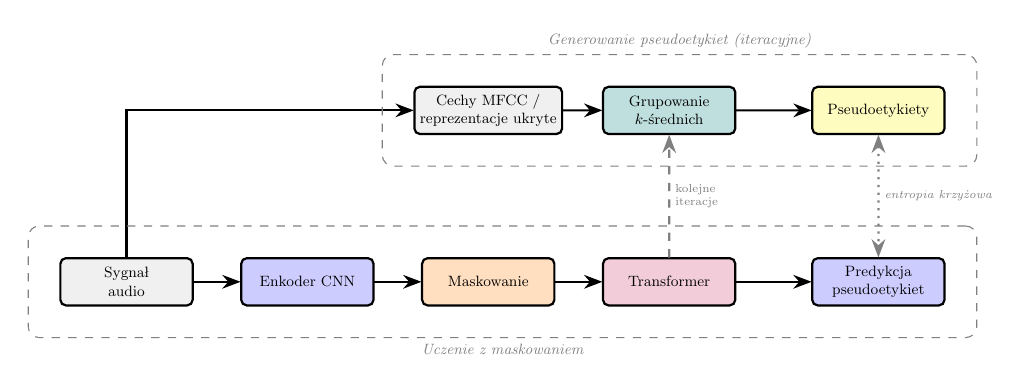
\begin{tikzpicture}[
    scale=0.6,
    transform shape,
    font=\small,
    block/.style={
        draw,
        rounded corners=2pt,
        thick,
        minimum width=2.8cm,
        minimum height=1.0cm,
        align=center
    },
    data/.style={block, fill=gray!12},
    model/.style={block, fill=blue!20},
    trans/.style={block, fill=purple!20},
    op/.style={block, fill=orange!25},
    clust/.style={block, fill=teal!25},
    lab/.style={block, fill=yellow!25},
    arrow/.style={-{Stealth[]}, thick},
    phase/.style={draw=gray, dashed, rounded corners=4pt, inner sep=0.4cm}
]

% ============================================================
% UCZENIE Z MASKOWANIEM
% ============================================================
\node[data] (audio) {Sygnał\\audio};
\node[model, right=1.0cm of audio] (cnn) {Enkoder CNN};
\node[op, right=1.0cm of cnn] (mask) {Maskowanie};
\node[trans, right=1.0cm of mask] (tr) {Transformer};
\node[model, right=1.6cm of tr] (pred) {Predykcja\\pseudoetykiet};

\draw[arrow] (audio) -- (cnn);
\draw[arrow] (cnn) -- (mask);
\draw[arrow] (mask) -- (tr);
\draw[arrow] (tr) -- (pred);

% ============================================================
% GENEROWANIE PSEUDOETYKIET
% ============================================================
\node[data, above=2.6cm of mask] (mfcc) {Cechy MFCC /\\reprezentacje ukryte};
\node[clust, above=2.6cm of tr] (km) {Grupowanie\\$k$-średnich};
\node[lab, above=2.6cm of pred] (pseudo) {Pseudoetykiety};

\draw[arrow] (audio.north) |- (mfcc.west);
\draw[arrow] (mfcc) -- (km);
\draw[arrow] (km) -- (pseudo);

% kolejne iteracje: reprezentacje transformera zasilają ponowne grupowanie
\draw[arrow, dashed, gray] (tr.north) --
    node[right, font=\scriptsize, text=gray, align=left] {kolejne\\iteracje} (km.south);

% cel predykcji
\draw[{Stealth[]}-{Stealth[]}, dotted, thick, gray] (pseudo.south) --
    node[right, font=\scriptsize\itshape, text=gray] {entropia krzyżowa} (pred.north);

% ============================================================
% RAMKI FAZ
% ============================================================
\node[phase, fit=(mfcc)(pseudo),
      label={[font=\small\itshape, gray]above:Generowanie pseudoetykiet (iteracyjne)}] {};
\node[phase, fit=(audio)(pred),
      label={[font=\small\itshape, gray]below:Uczenie z maskowaniem}] {};

\end{tikzpicture}

    \caption{Architektura modelu HuBERT. Pseudoetykiety powstają przez grupowanie $k$-średnich cech MFCC (pierwsza iteracja), a w kolejnych iteracjach -- reprezentacji ukrytych wytrenowanego modelu. Model uczy się przewidywać pseudoetykiety zamaskowanych segmentów.}
    \label{fig:hubertArchitecture}
\end{figure}

\subsubsection{Whisper}

Model Whisper \cite{whisper} reprezentuje odmienne podejście, oparte na uczeniu nadzorowanym w dużej skali. Model został wytrenowany na zbiorze 680 tysięcy godzin transkrybowanych nagrań audio pozyskanych z internetu, obejmujących 99 języków. Architektura Whisper składa się z enkodera i dekodera, oba oparte na transformerze.

W przeciwieństwie do modelu Wav2Vec 2.0, Whisper operuje na spektogramach w skali melowej. Stanowią one reprezentację częstotliwościową sygnału audio uwzględniającą charakterystykę ludzkiego słuchu. Takie podejście umożliwia normalizację dynamiki i redukcję szumu na etapie ekstrakcji cech, a jednocześnie przenosi ciężar modelowania z niskopoziomowych cech akustycznych na wyższe zależności językowe i kontekstowe. Enkoder przetwarza melspektrogram i generuje sekwencję reprezentacji ukrytych. Dekoder, działający w sposób autoregresyjny, generuje kolejne tokeny tekstu na podstawie reprezentacji z enkodera oraz wcześniej wygenerowanych tokenów. Schemat architektury przedstawiono na Rysunku \ref{fig:whisperArchitecture}.

Istotną cechą modelu Whisper jest uczenie wielozadaniowe (ang. \textit{multitask learning}). Model jest trenowany równocześnie do realizacji kilku zadań: transkrypcji mowy, detekcji języka, znaczników czasowych oraz tłumaczenia mowy na język angielski. Zadanie jest specyfikowane poprzez specjalne tokeny kontrolne umieszczane na początku sekwencji wyjściowej.

Zaletą modelu Whisper jest gotowość do użycia bez konieczności dostrajania (ang. \textit{zero-shot}). Dzięki treningowi na zróżnicowanym zbiorze danych model wykazuje odporność na szum, różne warunki akustyczne oraz akcenty. Wielojęzyczność modelu pozwala na transkrypcję nagrań w wielu językach, w tym w języku polskim, bez dodatkowej adaptacji.

\begin{figure}[htbp]
    \centering
    \begin{tikzpicture}[
    scale=0.6,
    transform shape,
    font=\small,
    block/.style={
        draw,
        rounded corners=2pt,
        thick,
        minimum width=2.8cm,
        minimum height=1.0cm,
        align=center
    },
    data/.style={block, fill=gray!12},
    feat/.style={block, fill=orange!25},
    enc/.style={block, fill=blue!20},
    dec/.style={block, fill=purple!20},
    ctrl/.style={block, fill=teal!25},
    arrow/.style={-{Stealth[]}, thick},
    phase/.style={draw=gray, dashed, rounded corners=4pt, inner sep=0.4cm}
]

\node[data] (audio) {Sygnał\\audio};
\node[feat, right=1.0cm of audio] (mel) {Melspektrogram};
\node[enc, right=1.0cm of mel] (enc) {Enkoder\\(Transformer)};
\node[data, right=1.0cm of enc] (hid) {Reprezentacje\\ukryte};
\node[dec, right=2.8cm of hid] (dec) {Dekoder\\(autoregresyjny)};
\node[data, right=1.6cm of dec] (out) {Tokeny wyjściowe\\(tekst)};

\draw[arrow] (audio) -- (mel);
\draw[arrow] (mel) -- (enc);
\draw[arrow] (enc) -- (hid);
\draw[arrow] (hid) -- node[above, font=\scriptsize] {\textit{cross-attention}} (dec);
\draw[arrow] (dec) -- (out);

% tokeny kontrolne zadania
\node[ctrl, below=2.2cm of dec] (ctrl)
    {Tokeny kontrolne\\(język, zadanie, znaczniki)};
\draw[arrow] (ctrl) -- (dec);

% sprzężenie autoregresyjne
\draw[arrow, gray] (out.north) -- ++(0,1.0)
    -| node[pos=0.25, above, font=\scriptsize, text=gray] {poprzednie tokeny (autoregresja)} (dec.north);

\end{tikzpicture}

    \caption{Architektura modelu Whisper. Enkoder przetwarza melspektrogram, a autoregresyjny dekoder generuje kolejne tokeny na podstawie reprezentacji enkodera, tokenów kontrolnych określających zadanie oraz wcześniej wygenerowanych tokenów.}
    \label{fig:whisperArchitecture}
\end{figure}

\subsubsection{Data2Vec}

Model Data2Vec \cite{data2vec} stanowi uogólnienie podejść do uczenia samonadzorowanego, oferując zunifikowaną architekturę zdolną do przetwarzania różnych modalności: mowy, obrazów oraz tekstu. Kluczową innowacją jest rezygnacja z przewidywania celów specyficznych dla modalności na rzecz predykcji kontekstowych reprezentacji latentnych.

Architektura Data2Vec opiera się na mechanizmie samodestylacji z wykorzystaniem modelu nauczyciela (ang. \textit{teacher}) oraz ucznia (ang. \textit{student}). Model nauczyciela przetwarza pełne dane wejściowe i generuje reprezentacje latentne. Model ucznia, otrzymując zamaskowane dane, przewiduje reprezentacje wygenerowane przez nauczyciela dla zamaskowanych fragmentów. Wagi nauczyciela są aktualizowane jako wykładnicza średnia krocząca (EMA) wag ucznia, co zapewnia stabilność procesu uczenia. Schemat architektury przedstawiono na Rysunku \ref{fig:data2vecArchitecture}.

W przypadku mowy Data2Vec wykorzystuje architekturę transformera analogiczną do Wav2Vec 2.0. Eksperymenty na zbiorze LibriSpeech wykazały, że model osiąga niższy wskaźnik WER niż Wav2Vec 2.0 i HuBERT, szczególnie przy ograniczonej ilości danych etykietowanych \cite{data2vec}. Zunifikowane podejście do uczenia upraszcza rozwój modeli multimodalnych i umożliwia transfer wiedzy między modalnościami.

\begin{figure}[htbp]
    \centering
    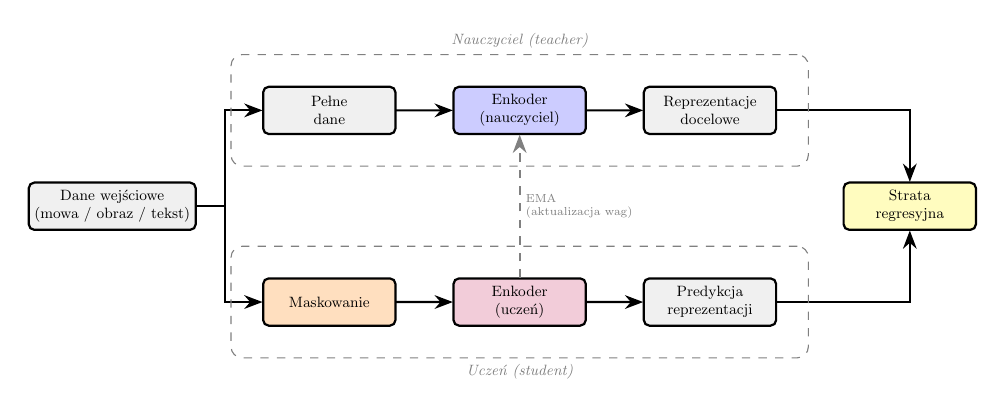
\begin{tikzpicture}[
    scale=0.6,
    transform shape,
    font=\small,
    block/.style={
        draw,
        rounded corners=2pt,
        thick,
        minimum width=2.8cm,
        minimum height=1.0cm,
        align=center
    },
    data/.style={block, fill=gray!12},
    teach/.style={block, fill=blue!20},
    stud/.style={block, fill=purple!20},
    op/.style={block, fill=orange!25},
    loss/.style={block, fill=yellow!25},
    arrow/.style={-{Stealth[]}, thick},
    phase/.style={draw=gray, dashed, rounded corners=4pt, inner sep=0.4cm}
]

% ============================================================
% WSPÓLNE WEJŚCIE
% ============================================================
\node[data] (src) {Dane wejściowe\\(mowa / obraz / tekst)};

% ============================================================
% GAŁĄŹ NAUCZYCIELA
% ============================================================
\node[data, above right=1.0cm and 1.4cm of src] (full) {Pełne\\dane};
\node[teach, right=1.2cm of full] (enct) {Enkoder\\(nauczyciel)};
\node[data, right=1.2cm of enct] (rept) {Reprezentacje\\docelowe};

\draw[arrow] (src.east) -- ++(0.6,0) |- (full.west);
\draw[arrow] (full) -- (enct);
\draw[arrow] (enct) -- (rept);

% ============================================================
% GAŁĄŹ UCZNIA
% ============================================================
\node[op, below right=1.0cm and 1.4cm of src] (mask) {Maskowanie};
\node[stud, right=1.2cm of mask] (encs) {Enkoder\\(uczeń)};
\node[data, right=1.2cm of encs] (preds) {Predykcja\\reprezentacji};

\draw[arrow] (src.east) -- ++(0.6,0) |- (mask.west);
\draw[arrow] (mask) -- (encs);
\draw[arrow] (encs) -- (preds);

% ============================================================
% STRATA I AKTUALIZACJA EMA
% ============================================================
\node[loss, right=1.4cm of rept.east |- src] (loss) {Strata\\regresyjna};

\draw[arrow] (rept.east) -| (loss.north);
\draw[arrow] (preds.east) -| (loss.south);

\draw[arrow, dashed, gray] (encs.north) --
    node[right, font=\scriptsize, text=gray, align=left] {EMA\\(aktualizacja wag)} (enct.south);

% ============================================================
% RAMKI GAŁĘZI
% ============================================================
\node[phase, fit=(full)(rept),
      label={[font=\small\itshape, gray]above:Nauczyciel (\textit{teacher})}] {};
\node[phase, fit=(mask)(preds),
      label={[font=\small\itshape, gray]below:Uczeń (\textit{student})}] {};

\end{tikzpicture}

    \caption{Architektura modelu Data2Vec. Nauczyciel przetwarza pełne dane wejściowe i wyznacza kontekstowe reprezentacje latentne stanowiące cel predykcji, natomiast uczeń otrzymuje dane zamaskowane. Wagi nauczyciela są wykładniczą średnią kroczącą (EMA) wag ucznia.}
    \label{fig:data2vecArchitecture}
\end{figure}

\subsection{Adaptacja do domeny specjalistycznej}

Pomimo wysokiej jakości modeli ogólnego przeznaczenia, zastosowania w domenach specjalistycznych wymagają często dodatkowej adaptacji. Terminologia medyczna, prawnicza czy techniczna jest słabo reprezentowana w ogólnych zbiorach treningowych, co prowadzi do błędów rozpoznawania specjalistycznych terminów.

Przykładem takiej adaptacji jest projekt ADMEDVoice \cite{ADMEDVoice}, w ramach którego przeprowadzono dostrajanie modelu Whisper Medium do transkrypcji polskiej mowy medycznej. Zbiór treningowy obejmował nagrania 28 mówców w różnych scenariuszach akustycznych, zawierające terminologię kliniczną. Dostrajanie pozwoliło na redukcję wskaźnika błędu słów (ang. \textit{Word Error Rate}, WER) z 24\% do 9,5\%, co stanowi znaczącą poprawę jakości transkrypcji w domenie medycznej.

Wyniki te ilustrują znaczenie danych domenowych dla jakości systemów ASR w zastosowaniach specjalistycznych. Jednocześnie wskazują na wyzwanie związane z ograniczoną dostępnością takich zbiorów, szczególnie dla języków innych niż angielski.

Analogiczny problem dotyczy modeli embeddingowych i językowych. Rozwiązaniem jest adaptacja modeli do konkretnych domen poprzez dodatkowy trening na specjalistycznych korpusach. W dziedzinie przetwarzania języka naturalnego powstały modele takie jak BioBERT \cite{lee2020biobert}, pretrenowany na korpusach tekstów biomedycznych z PubMed, czy PubMedBERT \cite{gu2021domain}, trenowany od podstaw wyłącznie na tekstach z domeny biomedycznej. Modele te wykazują znacząco lepszą jakość w zadaniach związanych z tekstami medycznymi w porównaniu z modelami ogólnego przeznaczenia.

\subsection{Porównanie podejść}

Modele Wav2Vec 2.0, HuBERT oraz Whisper reprezentują różne podejścia do problemu ASR. Wav2Vec 2.0 i HuBERT wykorzystują uczenie samonadzorowane, co pozwala na efektywne wykorzystanie nieetykietowanych nagrań audio. Różnią się jednak metodą uczenia: Wav2Vec 2.0 stosuje uczenie kontrastywne, podczas gdy HuBERT opiera się na przewidywaniu pseudoetykiet w sposób analogiczny do modelu BERT. Whisper reprezentuje odmienne podejście, oferując wysoką jakość bez konieczności dostrajania dzięki treningowi nadzorowanemu na masywnym zbiorze danych.

Otwartym pytaniem pozostaje, czy reprezentacje ukryte generowane przez modele ASR zawierają informację semantyczną wykraczającą poza poziom akustyczny i fonetyczny. Zagadnienie to stanowi motywację dla badań nad bezpośrednim wykorzystaniem reprezentacji modeli ASR w zadaniach wyszukiwania informacji.


% ---------------------------------------------------
\section{Wyjaśnialność modeli wykorzystujących uczenie głębokie}

Modele oparte na uczeniu głębokim realizują odwzorowanie danych wejściowych na wyjściowe poprzez sekwencję nieliniowych transformacji, których pojedyncze parametry nie mają bezpośredniej interpretacji. Nurt badań określany jako wyjaśnialność (ang. \textit{explainability}) obejmuje szerokie spektrum metod, od atrybucji cech dla pojedynczej predykcji po analizę własności całych przestrzeni reprezentacji. Z perspektywy niniejszej pracy istotny jest wyłącznie ten drugi obszar. Pytanie badawcze nie dotyczy bowiem uzasadnienia konkretnej transkrypcji, lecz tego, jaka informacja jest zakodowana w reprezentacjach ukrytych enkodera modelu ASR oraz w jaki sposób można tę informację zmierzyć.

\subsection{Semantyczność reprezentacji}

Pojęcie semantycznej reprezentacji wywodzi się z hipotezy dystrybucyjnej sformułowanej przez Harrisa, zgodnie z którą znaczenie słowa wynika z kontekstów jego występowania \cite{harris1954distributional}. Hipoteza ta stanowiła podstawę modeli generujących statyczne osadzenia wektorowe, takich jak Word2Vec \cite{mikolov2013efficient, mikolov2013distributed}, w których relacje semantyczne odwzorowywane są przez zależności geometryczne między wektorami. Wprowadzenie architektury transformera \cite{vaswani2017attention} i modeli takich jak BERT \cite{devlin2019bert} pozwoliło na generowanie reprezentacji kontekstowych, a modele typu Sentence-BERT \cite{reimers2019sentence} rozszerzyły to podejście na poziom całych zdań.

Zasadniczą trudnością jest fakt, że semantyczność nie jest wielkością obserwowalną bezpośrednio. Reprezentacja wektorowa nie posiada etykiety opisującej zakodowane w niej znaczenie, wobec czego jej ocena wymaga metod pośrednich. W literaturze wyróżnić można trzy grupy takich metod: analizę geometrycznych własności przestrzeni reprezentacji, zadania probingowe wykorzystujące dodatkowy model nadzorowany oraz dekompozycję reprezentacji na interpretowalne komponenty.

\subsection{Geometria przestrzeni reprezentacji}

Analiza geometryczna opiera się na założeniu, że rozkład reprezentacji w przestrzeni wielowymiarowej odzwierciedla jakość zakodowanej w nich informacji. Ethayarajh wykazał, że reprezentacje kontekstowe modeli BERT, ELMo i GPT-2 zajmują wąski stożek przestrzeni, przez co podobieństwo kosinusowe dowolnych dwóch losowych reprezentacji przyjmuje wartości znacząco dodatnie \cite{cone}. Zjawisko to, określane jako anizotropia przestrzeni, ogranicza zdolność miar podobieństwa do rozróżniania przykładów. Gao et al. wskazali, że degeneracja reprezentacji stanowi systematyczną konsekwencję treningu modeli generatywnych z funkcją straty opartą na wiarygodności \cite{gao2019representation}.

W odpowiedzi na to zjawisko opracowano metody przetwarzania końcowego przywracające izotropię przestrzeni. Metoda \textit{All-but-the-Top} usuwa z reprezentacji rzut na główne składowe odpowiadające za dominującą wariancję \cite{abtt}, natomiast wybielanie przekształca rozkład reprezentacji do postaci o zerowej średniej i jednostkowej macierzy kowariancji \cite{whiteningbert}. Odmienny wariant tej koncepcji stanowi \textit{concept whitening}, w którym transformacja wbudowana jest w architekturę modelu, dzięki czemu poszczególne osie przestrzeni odpowiadają zadanym pojęciom \cite{whitening}.

Analiza geometryczna znajduje zastosowanie również w kontekście modeli wielomodalnych i wielojęzycznych. Liang et al. opisali zjawisko \textit{modality gap}, polegające na tym, że reprezentacje różnych modalności w modelach uczonych kontrastywnie zajmują rozłączne obszary wspólnej przestrzeni \cite{liang2022mind}. Chang et al. wykazali natomiast, że w modelach wielojęzycznych wyodrębnić można podprzestrzenie specyficzne dla poszczególnych języków oraz podprzestrzeń wspólną, kodującą informację niezależną od języka \cite{chang2022geometry}. Do porównywania reprezentacji generowanych przez różne warstwy lub różne modele wykorzystywane są miary oparte na analizie korelacji kanonicznej, takie jak SVCCA \cite{raghu2017svcca}, oraz miara CKA \cite{pmlr-v97-kornblith19a}.

Metody opisane w tej części stanowią bezpośrednią podstawę metodologii ewaluacji przyjętej w rozdziale \ref{sec:latent}, w którym reprezentacje modeli ASR poddane zostały analizie pod kątem anizotropii, wpływu przetwarzania końcowego oraz separacji przykładów semantycznie podobnych i odległych.

\subsection{Podejścia probingowe i dekompozycja reprezentacji}

Metody sondujące (ang. \textit{probing}) opierają się na prostym rozumowaniu: jeżeli w reprezentacji wytworzonej przez daną warstwę modelu zakodowana jest pewna informacja, powinna ona dać się z niej odczytać za pomocą nieskomplikowanego klasyfikatora. Skuteczność takiego klasyfikatora, najczęściej liniowego, staje się wówczas miarą tego, na ile badana własność jest w reprezentacji dostępna \cite{alain2017probes}. Conneau et al. przenieśli tę ideę na poziom całych zdań, opracowując zestaw zadań pozwalających sprawdzić, które własności lingwistyczne -- od długości zdania po głębokość drzewa składniowego -- zachowują osadzenia zdaniowe \cite{conneau2018cram}. Belinkov i Glass zwracają jednak uwagę na zasadnicze ograniczenie tego podejścia: powodzenie sondy świadczy wyłącznie o tym, że informacja w reprezentacji się znajduje, nie zaś o tym, że model rzeczywiście się nią posługuje \cite{belinkov2019analysis}.

W domenie mowy najistotniejszym przykładem analizy probingowej jest praca Pasada et al., w której zbadano kolejne warstwy modelu Wav2Vec 2.0 \cite{pasad2021layer}. Wykazano, że model wykazuje charakterystykę zbliżoną do autoenkodera, przy czym warstwy środkowe kodują informację fonetyczną i leksykalną w stopniu najwyższym, natomiast warstwy końcowe wracają w kierunku reprezentacji zbliżonych do wejściowych. Obserwacja ta ma bezpośrednie znaczenie dla doboru warstwy wykorzystywanej jako źródło reprezentacji w architekturze proponowanej w niniejszej pracy. Pokrewny kierunek badań zakłada wymuszenie interpretowalności już na poziomie architektury, poprzez dyskretyzację reprezentacji do skończonego inwentarza jednostek, który można zestawiać z kategoriami fonetycznymi. Zhou et al. porównali stosowane w tym celu warianty kwantyzacji wektorowej, analizując ich wpływ na jakość reprezentacji mowy \cite{Zhou2020ACO}.

Podejścia jakościowe koncentrują się na rozkładzie reprezentacji na komponenty poddające się interpretacji. Punktem wyjścia jest obserwacja, że pojedyncze neurony sieci są zazwyczaj polisemantyczne, to znaczy aktywują się w odpowiedzi na wiele niepowiązanych ze sobą zjawisk, co wynika ze zjawiska superpozycji cech w przestrzeni o ograniczonej wymiarowości. Bricken et al. wykazali, że rzadkie autoenkodery (ang. \textit{sparse autoencoders}, SAE) trenowane na aktywacjach modelu językowego pozwalają na rozłożenie ich na słownik cech znacznie bliższych monosemantyczności \cite{bricken2023monosemanticity}. Wyniki te zostały potwierdzone i rozszerzone w pracy Hubena et al., w której wykazano wyższą interpretowalność cech uzyskanych metodą SAE w porównaniu z alternatywnymi metodami dekompozycji \cite{huben2024sparse}.

Podejście to znajduje coraz szersze zastosowanie w domenie audio. Paek et al. zastosowali rzadkie autoenkodery do przestrzeni cech ukrytych modeli audio, wyodrębniając składowe odpowiadające interpretowalnym zjawiskom akustycznym i muzycznym \cite{paek2025learninginterpretablefeaturesaudio}. Varshavsky-Hassid et al. wykazali natomiast obecność semantycznie nacechowanych kierunków w przestrzeni cech ukrytych dyfuzyjnych modeli syntezy mowy \cite{varshavskyhassid2024semanticlatentspacediffusionbased}. Prace te wskazują, że przestrzenie cech ukrytych modeli przetwarzających mowę zawierają strukturę wykraczającą poza poziom akustyczny, co stanowi bezpośrednią motywację dla badań prowadzonych w niniejszej pracy.

\subsection{Wyjaśnialność w systemach wyszukiwania opartych na mowie}

W architekturze kaskadowej transkrypcja stanowi pośredni artefakt umożliwiający kontrolę działania systemu przez użytkownika. Architektura pomijająca etap transkrypcji tej możliwości nie oferuje, co stanowi jej istotne ograniczenie. Analiza reprezentacji stanowi częściową rekompensatę tego ograniczenia. Pozwala ona na uzasadniony dobór modelu ASR i warstwy stanowiącej źródło reprezentacji, a także na diagnostykę własności przestrzeni wejściowej przed treningiem warstwy projekcji. Zestawienie metod omówionych w tej sekcji przedstawiono w Tabeli \ref{tab:xaiMetody}.

\begin{table}[htbp]
\centering
\small
\begin{tabular}{@{}L{4.0cm}L{6.6cm}L{3.2cm}@{}}
\toprule
\textbf{Metoda} & \textbf{Mierzona własność} & \textbf{Charakter} \\
\midrule
Klasyfikator probingowy & liniowa dostępność informacji w danej warstwie & ilościowy, nadzorowany \\
CKA, SVCCA & podobieństwo reprezentacji między warstwami i modelami & ilościowy \\
MMD na trypletach & separacja przykładów pozytywnych i negatywnych & ilościowy \\
Podobieństwo kosinusowe, efekt stożka & izotropia przestrzeni, dystans międzymodalny & ilościowy, geometryczny \\
ABTT, wybielanie & wpływ przetwarzania końcowego na zachowanie semantyki & ilościowy \\
Rzadkie autoenkodery (SAE) & interpretowalne składowe przestrzeni cech ukrytych & jakościowy \\
\bottomrule
\end{tabular}
\caption{Metody analizy reprezentacji wykorzystywane do oceny ich semantyczności.}
\label{tab:xaiMetody}
\end{table}


% ---------------------------------------------------
\section{Systemy wyszukiwania informacji w oparciu o sygnał audio}

Rosnące zapotrzebowanie na interfejsy głosowe motywuje rozwój systemów wyszukiwania informacji zdolnych do przetwarzania zapytań audio. Tradycyjne podejście opiera się na architekturze kaskadowej: sygnał mowy jest najpierw transkrybowany przez system ASR, a następnie uzyskany tekst wykorzystywany jest w standardowym procesie wyszukiwania. Rozwiązanie to jest jednak podatne na propagację błędów rozpoznawania mowy, szczególnie w przypadku terminologii specjalistycznej, różnych akcentów lub nagrań niskiej jakości.

W odpowiedzi na te ograniczenia powstały dwa główne nurty badawcze. Pierwszy koncentruje się na architekturach end-to-end, które uczą się bezpośredniego mapowania sygnału audio na reprezentacje semantyczne, omijając etap transkrypcji. Drugi wykorzystuje podejścia multimodalne, tworzące wspólną przestrzeń reprezentacji dla danych audio, tekstowych i obrazu.

\subsection{Podejścia end-to-end}

\textbf{SpeechDPR.} Model SpeechDPR (ang. \textit{Speech Dense Passage Retriever}) \cite{lin2024speechdprendtoendspokenpassage} stanowi pierwsze rozwiązanie typu end-to-end dla problemu wyszukiwania fragmentów mowy w zadaniach odpowiadania na pytania. Model uczy się semantycznych reprezentacji na poziomie zdaniowym poprzez destylację wiedzy z systemu kaskadowego składającego się z nienadzorowanego ASR oraz tekstowego retriever'a opartego na gęstych reprezentacjach. Proces ten nie wymaga ręcznie transkrybowanych danych mowy, co stanowi istotną zaletę w kontekście języków o ograniczonych zasobach. Schemat procesu treningu przedstawiono na Rysunku \ref{fig:speechdprArchitecture}.

\begin{figure}[htbp]
    \centering
    \begin{tikzpicture}[
    scale=0.6,
    transform shape,
    font=\small,
    block/.style={
        draw,
        rounded corners=2pt,
        thick,
        minimum width=2.8cm,
        minimum height=1.0cm,
        align=center
    },
    data/.style={block, fill=gray!12},
    model/.style={block, fill=blue!20},
    txt/.style={block, fill=purple!20},
    stud/.style={block, fill=teal!25},
    loss/.style={block, fill=yellow!25},
    arrow/.style={-{Stealth[]}, thick},
    phase/.style={draw=gray, dashed, rounded corners=4pt, inner sep=0.4cm}
]

% ============================================================
% WSPÓLNE WEJŚCIE
% ============================================================
\node[data] (src) {Audio zapytań\\i fragmentów};

% ============================================================
% NAUCZYCIEL: SYSTEM KASKADOWY
% ============================================================
\node[model, above right=1.2cm and 1.4cm of src] (asr) {Nienadzorowany\\model ASR};
\node[data, right=1.2cm of asr] (text) {Tekst};
\node[txt, right=1.2cm of text] (dpr) {Tekstowy retriever\\(DPR)};
\node[data, right=1.2cm of dpr] (scoret) {Oceny\\podobieństwa};

\draw[arrow] (src.east) -- ++(0.6,0) |- (asr.west);
\draw[arrow] (asr) -- (text);
\draw[arrow] (text) -- (dpr);
\draw[arrow] (dpr) -- (scoret);

% ============================================================
% UCZEŃ: SPEECHDPR
% ============================================================
\node[stud, below right=1.2cm and 1.4cm of src] (enc) {Enkoder mowy\\(SpeechDPR)};
\node[data, right=1.2cm of enc] (rep) {Reprezentacje\\zdaniowe};
\node[data, right=1.2cm of rep] (scores) {Podobieństwo\\kosinusowe};

\draw[arrow] (src.east) -- ++(0.6,0) |- (enc.west);
\draw[arrow] (enc) -- (rep);
\draw[arrow] (rep) -- (scores);

% ============================================================
% STRATA DESTYLACYJNA
% ============================================================
\node[loss, right=1.4cm of scoret.east |- src] (loss) {Strata\\destylacyjna};

\draw[arrow] (scoret.east) -| (loss.north);
\draw[arrow] (scores.east) -| (loss.south);

% ============================================================
% RAMKI
% ============================================================
\node[phase, fit=(asr)(scoret),
      label={[font=\small\itshape, gray]above:Nauczyciel -- system kaskadowy (bez ręcznych transkrypcji)}] {};
\node[phase, fit=(enc)(scores),
      label={[font=\small\itshape, gray]below:Uczeń -- model end-to-end}] {};

\end{tikzpicture}

    \caption{Schemat treningu modelu SpeechDPR. Kaskadowy nauczyciel, złożony z nienadzorowanego modelu ASR i tekstowego retrievera, dostarcza ocen podobieństwa stanowiących cel destylacji dla enkodera mowy uczonego bezpośrednio na sygnale audio.}
    \label{fig:speechdprArchitecture}
\end{figure}

\textbf{SpeechRAG.} SpeechRAG \cite{min2025speechretrievalaugmentedgenerationautomatic} rozszerza architekturę RAG o bezpośrednie przetwarzanie audio. System składa się z retriever'a audio oraz generatora opartego na modelu języka mowy (SLM, ang. \textit{Speech Language Model}). Kluczową innowacją jest dostrojenie pretrenowanego enkodera mowy do roli adaptera podłączonego do zamrożonego retriever'a tekstowego. Dzięki wyrównaniu przestrzeni embeddingów retriever audio może wyszukiwać fragmenty na podstawie zapytań tekstowych. W fazie generacji model SLM otrzymuje jako kontekst oryginalne fragmenty audio, eliminując straty informacyjne wynikające z konwersji mowa-tekst. Architekturę systemu przedstawiono na Rysunku \ref{fig:speechragArchitecture}.

\begin{figure}[htbp]
    \centering
    \begin{tikzpicture}[
    scale=0.6,
    transform shape,
    font=\small,
    block/.style={
        draw,
        rounded corners=2pt,
        thick,
        minimum width=2.8cm,
        minimum height=1.0cm,
        align=center
    },
    data/.style={block, fill=gray!12},
    adapt/.style={block, fill=teal!25},
    frozen/.style={block, fill=blue!20},
    store/.style={block, fill=orange!25},
    ann/.style={block, fill=yellow!25},
    gen/.style={block, fill=green!20},
    arrow/.style={-{Stealth[]}, thick},
    phase/.style={draw=gray, dashed, rounded corners=4pt, inner sep=0.4cm}
]

% ============================================================
% FAZA WYSZUKIWANIA
% ============================================================
\node[data] (query) {Zapytanie\\tekstowe};
\node[frozen, right=1.8cm of query] (enct) {Enkoder tekstu\\(zamrożony)};
\node[data, right=1.8cm of enct] (qvec) {Wektor\\zapytania};
\node[ann, right=1.8cm of qvec] (search) {Wyszukiwanie ANN};

\draw[arrow] (query) -- (enct);
\draw[arrow] (enct) -- (qvec);
\draw[arrow] (qvec) -- (search);

% ============================================================
% FAZA INDEKSOWANIA
% ============================================================
\node[data, above=2.6cm of query] (chunks) {Fragmenty\\audio};
\node[adapt, above=2.6cm of enct] (adapter) {Enkoder mowy --\\adapter (trenowany)};
\node[store, above=2.6cm of search] (db) {Wektorowa\\baza danych};

\draw[arrow] (chunks) -- (adapter);
\draw[arrow] (adapter) -- (db);
\draw[arrow] (db) -- node[right, font=\scriptsize] {indeks} (search);

% wyrównanie przestrzeni embeddingów
\draw[{Stealth[]}-{Stealth[]}, dotted, thick, gray] (enct.north) --
    node[left, pos=0.78, font=\scriptsize\itshape, text=gray]
    {wspólna przestrzeń} (adapter.south);

% ============================================================
% FAZA GENERACJI
% ============================================================
\node[data, below=2.6cm of query] (topk) {Top-$k$ fragmentów\\audio};
\node[gen, right=2.6cm of topk] (slm) {Model języka mowy\\(SLM)};
\node[data, right=1.8cm of slm] (ans) {Odpowiedź};

\draw[arrow] (search.south) -- ++(0,-0.8) -| (topk.north);
\draw[arrow] (topk) -- node[above, font=\scriptsize] {kontekst audio} (slm);
\draw[arrow] (slm) -- (ans);

% ============================================================
% RAMKI FAZ
% ============================================================
\node[phase, fit=(chunks)(db),
      label={[font=\small\itshape, gray]above:Faza indeksowania}] {};
\node[phase, fit=(query)(search),
      label={[font=\small\itshape, gray]above left:Faza wyszukiwania}] {};
\node[phase, fit=(topk)(ans),
      label={[font=\small\itshape, gray]below left:Faza generacji}] {};

\end{tikzpicture}

    \caption{Architektura systemu SpeechRAG. Enkoder mowy pełniący rolę adaptera jest dostrajany tak, aby fragmenty audio trafiały do przestrzeni wektorowej zamrożonego enkodera tekstu. Wyszukane fragmenty audio stanowią bezpośredni kontekst modelu języka mowy.}
    \label{fig:speechragArchitecture}
\end{figure}

\subsection{Podejścia multimodalne}

Budowa systemów wyszukiwania opartych na wspólnej przestrzeni reprezentacji dla audio i tekstu jest ułatwiona dzięki modelom takim jak Data2Vec (opisany w podrozdziale \ref{sec:modeleASR}), które oferują zunifikowane podejście do uczenia reprezentacji różnych modalności.

\textbf{WavRAG.} WavRAG \cite{wavRAG} umożliwia reprezentowanie sygnałów audio w tej samej przestrzeni semantycznej co dane tekstowe. Pozwala to na pełną integrację informacji mówionej i pisanej w ramach jednego systemu. Zapytania głosowe są kodowane jako wektory w przestrzeni cech ukrytych, a wyszukiwanie opiera się na bezpośrednim dopasowywaniu embeddingów akustycznych i tekstowych za pomocą podobieństwa kosinusowego. Architekturę systemu przedstawiono na Rysunku \ref{fig:wavragArchitecture}.

\begin{figure}[htbp]
    \centering
    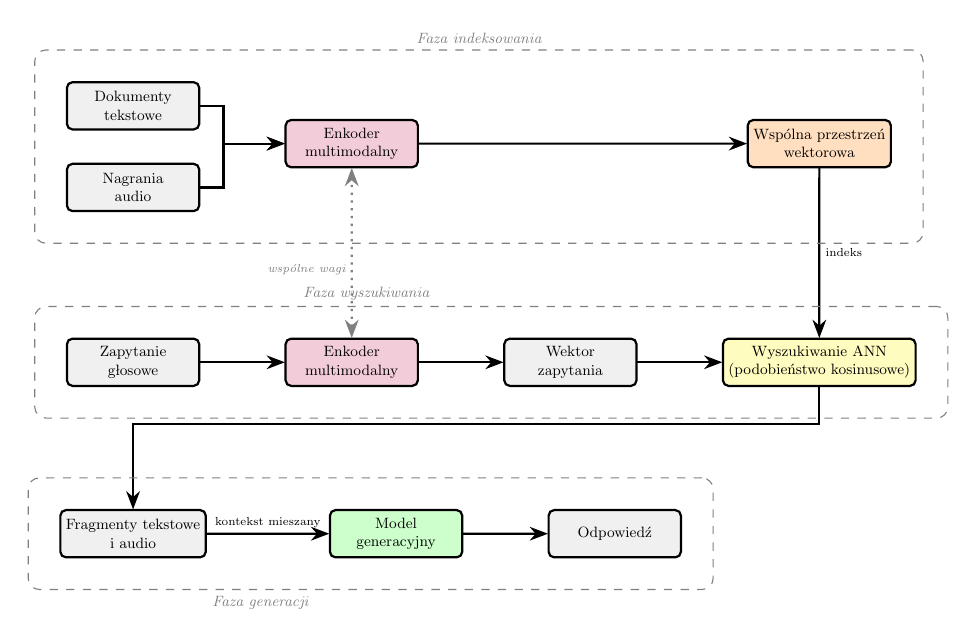
\begin{tikzpicture}[
    scale=0.6,
    transform shape,
    font=\small,
    block/.style={
        draw,
        rounded corners=2pt,
        thick,
        minimum width=2.8cm,
        minimum height=1.0cm,
        align=center
    },
    data/.style={block, fill=gray!12},
    embm/.style={block, fill=purple!20},
    store/.style={block, fill=orange!25},
    ann/.style={block, fill=yellow!25},
    gen/.style={block, fill=green!20},
    arrow/.style={-{Stealth[]}, thick},
    phase/.style={draw=gray, dashed, rounded corners=4pt, inner sep=0.4cm}
]

% ============================================================
% FAZA WYSZUKIWANIA
% ============================================================
\node[data] (query) {Zapytanie\\głosowe};
\node[embm, right=1.8cm of query] (encq) {Enkoder\\multimodalny};
\node[data, right=1.8cm of encq] (qvec) {Wektor\\zapytania};
\node[ann, right=1.8cm of qvec] (search) {Wyszukiwanie ANN\\(podobieństwo kosinusowe)};

\draw[arrow] (query) -- (encq);
\draw[arrow] (encq) -- (qvec);
\draw[arrow] (qvec) -- (search);

% ============================================================
% FAZA INDEKSOWANIA
% ============================================================
\node[data, above=4.4cm of query] (docs) {Dokumenty\\tekstowe};
\node[data, below=0.7cm of docs] (recs) {Nagrania\\audio};
\node[embm, above=3.6cm of encq] (enci) {Enkoder\\multimodalny};
\node[store, above=3.6cm of search] (db) {Wspólna przestrzeń\\wektorowa};

\draw[arrow] (docs.east) -- ++(0.5,0) |- (enci.west);
\draw[arrow] (recs.east) -- ++(0.5,0) |- (enci.west);
\draw[arrow] (enci) -- (db);
\draw[arrow] (db) -- node[right, font=\scriptsize] {indeks} (search);

% wspólne wagi enkodera dla obu faz
\draw[{Stealth[]}-{Stealth[]}, dotted, thick, gray] (encq.north) --
    node[left, pos=0.4, font=\scriptsize\itshape, text=gray] {wspólne wagi} (enci.south);

% ============================================================
% FAZA GENERACJI
% ============================================================
\node[data, below=2.6cm of query] (topk) {Fragmenty tekstowe\\i audio};
\node[gen, right=2.6cm of topk] (gen) {Model\\generacyjny};
\node[data, right=1.8cm of gen] (ans) {Odpowiedź};

\draw[arrow] (search.south) -- ++(0,-0.8) -| (topk.north);
\draw[arrow] (topk) -- node[above, font=\scriptsize] {kontekst mieszany} (gen);
\draw[arrow] (gen) -- (ans);

% ============================================================
% RAMKI FAZ
% ============================================================
\node[phase, fit=(docs)(recs)(enci)(db),
      label={[font=\small\itshape, gray]above:Faza indeksowania}] {};
\node[phase, fit=(query)(search),
      label={[font=\small\itshape, gray]above left:Faza wyszukiwania}] {};
\node[phase, fit=(topk)(ans),
      label={[font=\small\itshape, gray]below left:Faza generacji}] {};

\end{tikzpicture}

    \caption{Architektura systemu WavRAG. Ten sam enkoder multimodalny obsługuje obie modalności, dzięki czemu dokumenty tekstowe i nagrania audio trafiają do wspólnej przestrzeni wektorowej, a wyszukane fragmenty obu typów stanowią kontekst modelu generacyjnego.}
    \label{fig:wavragArchitecture}
\end{figure}

\textbf{Wyszukiwanie multimodalne dla ASR.} Kolehmainen et al. \cite{kolehmainen2024multimodalretrievallargelanguage} zbadali zastosowanie wyszukiwania multimodalnego do poprawy jakości rozpoznawania mowy. Zaproponowany system wykorzystuje dwie techniki: kNN-LM (ang. \textit{k-Nearest Neighbors Language Model}) oraz mechanizmy cross-attention. Wyszukiwanie oparte na mowie prowadzi do redukcji WER o nawet 50\% w porównaniu z bazowym modelem. System osiągnął wyniki state-of-the-art w zadaniu rozpoznawania mowy na zbiorze Spoken-Squad. Sposób włączenia wyszukanych fragmentów do procesu rozpoznawania przedstawiono na Rysunku \ref{fig:multimodalAsrArchitecture}.

\begin{figure}[htbp]
    \centering
    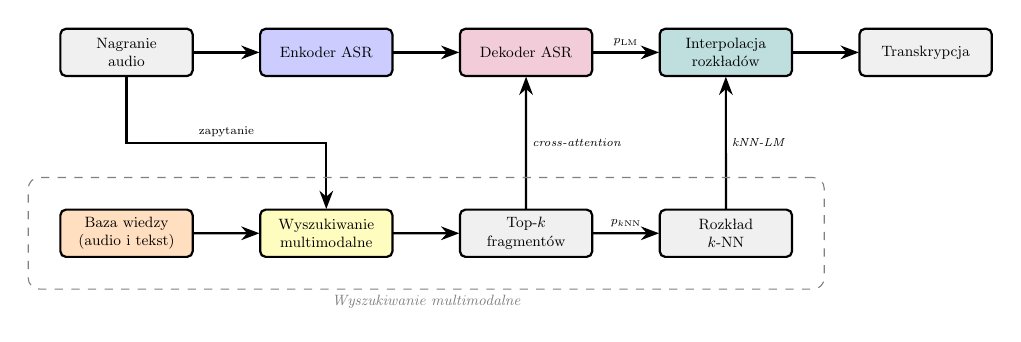
\begin{tikzpicture}[
    scale=0.6,
    transform shape,
    font=\small,
    block/.style={
        draw,
        rounded corners=2pt,
        thick,
        minimum width=2.8cm,
        minimum height=1.0cm,
        align=center
    },
    data/.style={block, fill=gray!12},
    model/.style={block, fill=blue!20},
    dec/.style={block, fill=purple!20},
    ret/.style={block, fill=yellow!25},
    store/.style={block, fill=orange!25},
    fuse/.style={block, fill=teal!25},
    arrow/.style={-{Stealth[]}, thick},
    phase/.style={draw=gray, dashed, rounded corners=4pt, inner sep=0.4cm}
]

% ============================================================
% ŚCIEŻKA ROZPOZNAWANIA MOWY
% ============================================================
\node[data] (audio) {Nagranie\\audio};
\node[model, right=1.4cm of audio] (enc) {Enkoder ASR};
\node[dec, right=1.4cm of enc] (dec) {Dekoder ASR};
\node[fuse, right=1.4cm of dec] (interp) {Interpolacja\\rozkładów};
\node[data, right=1.4cm of interp] (text) {Transkrypcja};

\draw[arrow] (audio) -- (enc);
\draw[arrow] (enc) -- (dec);
\draw[arrow] (dec) -- node[above, font=\scriptsize] {$p_{\mathrm{LM}}$} (interp);
\draw[arrow] (interp) -- (text);

% ============================================================
% ŚCIEŻKA WYSZUKIWANIA MULTIMODALNEGO
% ============================================================
\node[store, below=2.8cm of audio] (kb) {Baza wiedzy\\(audio i tekst)};
\node[ret, below=2.8cm of enc] (ret) {Wyszukiwanie\\multimodalne};
\node[data, below=2.8cm of dec] (topk) {Top-$k$\\fragmentów};
\node[data, below=2.8cm of interp] (knn) {Rozkład\\$k$-NN};

\draw[arrow] (kb) -- (ret);
\draw[arrow] (ret) -- (topk);
\draw[arrow] (topk) -- node[above, font=\scriptsize] {$p_{k\mathrm{NN}}$} (knn);

\draw[arrow] (audio.south) -- ++(0,-1.4)
    -| node[pos=0.25, above, font=\scriptsize] {zapytanie} (ret.north);

% ============================================================
% MECHANIZMY INTEGRACJI
% ============================================================
\draw[arrow, thick] (topk.north) --
    node[right, font=\scriptsize\itshape] {\textit{cross-attention}} (dec.south);
\draw[arrow, thick] (knn.north) --
    node[right, font=\scriptsize\itshape] {kNN-LM} (interp.south);

\node[phase, fit=(kb)(knn),
      label={[font=\small\itshape, gray]below:Wyszukiwanie multimodalne}] {};

\end{tikzpicture}

    \caption{Wyszukiwanie multimodalne wspierające rozpoznawanie mowy. Wyszukane fragmenty oddziałują na model ASR dwiema drogami: poprzez mechanizm uwagi krzyżowej w dekoderze oraz poprzez interpolację rozkładu prawdopodobieństwa tokenów z rozkładem wyznaczonym metodą $k$-NN.}
    \label{fig:multimodalAsrArchitecture}
\end{figure}

\subsection{Charakterystyka i porównanie podejść}

Przedstawione podejścia łączy dążenie do eliminacji lub ograniczenia roli tradycyjnego ASR jako pośredniego etapu przetwarzania. Zarówno architektury end-to-end, jak i multimodalne wykazują przewagę nad systemami kaskadowymi w warunkach niskiej jakości rozpoznawania mowy. Bezpośrednie uczenie reprezentacji semantycznych z sygnału audio przynosi dwie kluczowe korzyści: redukuje propagację błędów transkrypcji oraz otwiera możliwość zachowania informacji prozodycznych i paralingwistycznych, traconych w procesie konwersji mowa-tekst. Żadna z omówionych prac nie wykazuje jednak, by informacja prozodyczna była w tych systemach faktycznie wykorzystywana przy wyszukiwaniu. Stanowi to fundamentalną zmianę paradygmatu w projektowaniu systemów wyszukiwania informacji opartych na danych mowy.


% Badanie latent space
\chapter{Semantyczne reprezentacje wektorów cech modeli ASR\aut{T.P.}}
\label{sec:latent}
\subsection{Założenia teorytyczne}
\subsubsection{Semantyczne a syntaktyczne reprezentacje audio w wektorach cech}
Dla proponowanego przez nas rozwiązanie, potencjalnie najważniejszą charakterystyką, którą wykazują się dostępne modele ASR jest postać ukrytej (latentnej) reperezentacji enkodowanej przez nie na podstawie danych wejściowych. Potencjalnie, większa wierność semantycznemu znaczeniu wypowiedzianego zdania doprowadzi do dokładniejszej translacji wyjścia enkodera na współdzielną przestrzeń embeddingów, czego konsekwencją będą lepsze osiągi systemu wyszukiwania dla użytkownika końcowego.
\subsubsection{Wpływ charakterystyki wektorów cech na jakość embeddingów w modelach wielojęzykowych}
Kolejnym aspektem ewaluowanym przez nas w ramach eksperymentu są podobieństwa wyników modeli dla zdań o tym samym znaczeniu w kilku językach. Dla modeli enkodujących semantykę danych, reprezentacje dla dwóch znaczeniowo identycznych zdań w dwóch różnych językach powinny być do siebie podobne według przyjętej metryki podobieństwa. Przykładowo, miara podobieństwa dla reprezentacji latentnych dla zdań "Kocham zwiedzać włoskie miasta" i "I love sightseeing Italian cities", dla modelu semantycznego, powinna mieć jak największą wartość.

Należy mieć na uwadze, że różnice w historii języka, jego strukturze i alfabecie istotnie wpływają na otrzymane wyniki podobieństwa dla takich zdań. Zróżnicowanie to zostało zbadane przez Aleshinę et. al w ich pracy ewaluującej rozkłady embeddingów zdań dla dziesięciu różnych języków \cite{multilanguageEmbeddingDifferences}. Korzystając z modelu MUSE \cite{museModel} operującego na pojedynczych słowach, wykazali oni znaczące pokrycie klastrów embeddingów dla języków o podobnej historii (arabski i hiszpański) jak i o podobnie prostej morfologii i częściowo współdzielonym słownictwie (angielski, chiński, indonezyjski), i izolację klastrów dla wybranych języków (rosyjski, o innym alfabecie i bardziej skomplikowanej morfologii w świetle inflekcji języka). Najbardziej interesującym dla nas wnioskiem są podobieństwa dla słów zapożyczonych z innych języków -- wiele terminów medycznych wywodzi się z języka łacińskiego, co oznacza potencjalnie wysokie podobieństwo dla takich zwrotów w języku angielskim i polskim, jak i w innych językach \cite{latinMedical}.

Wysoka miara podobieństwa dla modelu ASR ewaluowanego dla danych wielojęzykowych oznaczałaby nie tylko dobre radzenie sobie z samą semantyką wypowiedzianych zdań, lecz także potencjalnie wysoki potencjał do przeprowadzenia treningu modelu na specjalistycznych danych dostępnych w innych językach. Model wykazujący się taką cechą byłby niezwykle cenny dla poprawienia jakości wyszukiwania informacji dla nie tylko polskojęzycznych, ale również innych języków wspieranych przez ten model. Właśnie taki proces destylacji wiedzy zbadali w swojej pracy Piperno et. al \cite{multilingualDomainTranslation}, z powodzeniem korzystając z anglojęzycznych zbiorów słownictwa o tematyce medycznej do poprawienia osiągów modeli dla danych w językach hiszpańskim, niemieckim i francuskim. Przeprowadzony w ten sposób dodatkowy trening pozwoliłaby nam na znaczące polepszenie naszego całościowego rozwiązania, umożliwiając skorzystanie z większej ilości danych dostępnych w języku angielskim i przełożenia zdobytej przez model wiedzy na język polski dla zbioru ADMEDVoice \cite{ADMEDVoice}.


\subsection{Metodologia}
\subsubsection{Ocena jakości embeddingów}
W celu rzetelenej weryfikacji powyższej hipotezy dotyczącej semantyki w reprezentacjach latentnych modeli ASR, sformułowaliśmy eksperyment wykorzystujący istniejące modele embeddingowe dla tekstu wspierające wiele języków. Wykorzystując istniejące zbiory danych zawierające zarówno audio wypowiedzianego zdania, jak i jego transkrypcję, za ich pomocą wygenerowaliśmy przykłady treningowe dla każdego zdania inspirowane metodą \textit{triplet loss} \cite{tripletLoss}.

\begin{equation}
    \mathcal{L}_{\text{triplet}} = \max \Big( 0, \; \| f(x^a) - f(x^p) \|_2^2 - \| f(x^a) - f(x^n) \|_2^2 + \alpha \Big)
    \label{eq:tripletloss}
\end{equation}

Na początku dla transkrypcji każdego zdania w zbiorze danych wygenerowaliśmy jego embeddingi za pomocą każdego z ewaluowanych modeli embeddingowych. Następnie, dla każdego zdania (oznaczonego jako $x^a$ -- \textit{anchor}), wyliczyliśmy dystans (norma L2) do każdego z pozostałych zdań dla każdego modelu embeddingowego:

\begin{equation}
    D(x_{emb}^a, x_{emb}) = \| x_{emb}^a - x_{emb} \|_2^2 = \sqrt{(x_{emb}^a - x_{emb})^2}
\end{equation}

Następnie, na podstawie wygenerowanych w ten sposób zbiorów odległości, wybraliśmy losowo przykłady pozytywne $x^p$ i negatywne $x^n$. Przykłady pozytywne stanowiły losowe zdanie spośród najbliższych (najbardziej podobnych) dziesięciu przykładów, z kolei przykłady negatywne spośród najmniej podobnych czterdziestu procent zdań. Losowość miała na celu zapewnić stosunkowo równomierny rozkład przykładów negatywnych spośród całego zbioru danych.

Posiadając trzy przykłady $x^a$, $x^n$ i $x^p$ dla każdego unikalnego zdania w zbiorze, następnym krokiem było wygenerowanie embeddingów dla każdego z ewaluowanych modeli ASR. Następnie, porównywaliśmy je za pomocą metryki $m(x_1, x_2)$, otrzymując w rezultacie ewaluacje relatywnego podobieństwa między $x^a$ i kolejno $x^p$ i $x^n$:

\begin{equation}
    S(x_{emb, asr}) = m(x_{emb, asr}^a, x_{emb, asr}^n) - m(x_{emb, asr}^a, x_{emb, asr}^p)
    \label{eq:tripletDiff}
\end{equation}

Metryka, którą wykorzystaliśmy podczas tej ewaluacji to \textit{Maximum Mean Discrepancy} (MMD) \cite{mmd}. Jest ona przeznaczona do porównywania różnicy między dwoma dwuwymiarowymi tensorami, które stanowią w naszym przypadku embeddingi wygenerowane przez modele ASR. Jest ona wyrażana wzorem:
\begin{equation}
\widehat{\text{MMD}}^2(X,Y) =
\frac{1}{m^2} \sum_{i=1}^{m} \sum_{i'=1}^{m} k(x_i, x_{i'})
+ \frac{1}{n^2} \sum_{j=1}^{n} \sum_{j'=1}^{n} k(y_j, y_{j'})
- \frac{2}{mn} \sum_{i=1}^{m} \sum_{j=1}^{n} k(x_i, y_j)
\label{eq:MMD}
\end{equation}

Z racji określania różnicy zamiast podobieństwa między dwoma reprezentacjami, w ramach porównania opisanego równaniem \ref{eq:tripletDiff}, wartość ewaluacji $S(x_{emb, asr})$ będzie dodatnia, jeśli model poprawnie uchwycił relatywne podobieństwa semantyczne przykładów $x^a$, $x^n$ i $x^p$. W ten sposób możliwe jest ilościowe podejście do ewaluacji jakości w semantyczności reprezentacji modelu w ramach danego zbioru danych.

Ponadto, w celu zbadania rozkładu wartości ewaluacji $S(x_{emb, asr})$, dla zagregowanych w ramach modeli embeddingowych wyników dopasowaliśmy rozkład Student-t, dla którego funkcja gęstości prawdopodobieństwa jest wyrażana wzorem:

\begin{equation}
f(t; \nu, \mu, \sigma) =
\frac{\Gamma\!\left(\frac{\nu+1}{2}\right)}
     {\Gamma\!\left(\frac{\nu}{2}\right) \sqrt{\nu \pi}\, \sigma}
\left[ 1 + \frac{1}{\nu} \left( \frac{t - \mu}{\sigma} \right)^2 \right]^{-\frac{\nu+1}{2}}
\label{eq:studentT}
\end{equation}

Pozwala on na analizę statystyczną zachowania modeli w ramach naszego podejścia ilościowego, dostarczając informacji na temat stabilności i zdolności modelu do separacji przykładów pozytywnych i negatywnych, które są niezwykle cennymi czynnikami przy doborze właściwego modelu do dalszych eksperymentów.

\subsubsection{Analiza rozkładu embeddingów w przestrzeni}
Kolejnym krokiem analizy ilościowej jakości embeddingów generowanych przez modele ASR jest zbadanie obecności "efektu stożka \textit(cone effect)", opisanego w pracy \textit{Mind the Gap: Understanding the Modality Gap in Multi-modal Contrastive Representation Learning} \cite{liang2022mind}. Oryginalna praca skupia się na metodach badania różnicy w reprezentacji danych o różnej modalności w modelach embeddingowych. Głównym narzędziem proponowanym przez autorów jest badanie podobieństwa kosinusowego między embeddingami dla każdej z obsługiwanej przez model modalności. Niech $x^{(i)}$ oznacza dane wejściowe dla modalności $i$, $f_i$ model dla modalności $i$, $z^i$ znormalizowany embedding dla modalności $i$ i $s(x^{(i)}, x^{(j)})$ podobieństwo kosinusowe dla porównywanych modalności $i$ i $j$, wtedy:

\begin{equation}
z^{(1)} = \frac{f_1(x^{(1)})}{\left\| f_I(x^{(1)}) \right\|_2},
\quad
z^{(2)} = \frac{f_2(x^{(2)})}{\left\| f_T(x^{(2)}) \right\|_2},
\quad
s(x^{(1)}, x^{(2)}) = \left\langle z^{(1)}, z^{(2)} \right\rangle
\end{equation}

Z racji natury reprezentacji danych przez enkodery modeli ASR, będacych tensorami dwuwymiarowymi, aby uzyskać geometryczną reprezentację podobieństwa, należy uśrednić dane w ramach domeny czasu w ramach operacji \textit{mean pooling}. Niech $H \in \mathbb{R}^{n \times d}$ oznacza reprezentację ukrytą enkodera, $M \in \{0,1\}^{n \times 1}$ maskę atencji (\textit{attention mask}), i $1 \in \mathbb{R}^{n \times 1}$ wektor składający się z wartości $1$, wtedy wynik operacji \textit{mean pooling} $h_\text{mp}$ ma postać:

\begin{equation}
    h_{\text{mp}} =
    \frac{M^\top H}{1^\top M}
\end{equation}


Wyliczenia te pozwalają na zbadanie właściwości n-wymiarowego stożka, w którym znajdują się embeddingi wygenerowane przez model. Różnice między podobieństwem wewnątrz modalności a podobieństwem inter-modalnym pozwalają na analizę różnicy, według której model reaguje na różne rodzaje danych wejściowych.

Analiza ta nie jest przydatna tylko dla proponowanych przez nas modeli z rodziny speech-to-retrieval. W pracy \textit{The Geometry of Multilingual Language Model Representations}, autorzy badali również podobieństwo między reprezentacjami danych dla różnych języków obsługiwanych przez model językowy XLM-R \cite{chang2022geometry}. Rezultaty przedstawione przez autorów udowodniły, że podprzestrzenie zajmowane przez embeddingi poszczególnych języków są podobne do siebie, lecz przesunięte w hiperprzestrzeni.

Mając na uwadzę obie te prace, jak i cel naszej analizy, postanowiliśmy połączyć oba podejścia. Poprzez traktowanie języków jako modalności w świetle efektu stożka i mając na uwadzę potencjalne przesunięcia podprzestrzeni dla różnych języków w ramach dziedziny przetwarzania tekstu, zbadana została umiejętność kodowania znaczenia semantycznego mowy przez modele ASR w ramach przetwarzania danych wielojęzycznych.

W celu bardziej kompleksowego wpływu, jaki ma język danych na końcowy rozkład embeddingów modelu, zastosowaliśmy również zabieg wybielania \textit{(whitening)}, zaadaptowany z pracy \textit{Concept whitening for interpretable image recognition} \cite{whitening}. W tej pracy autorzy zaproponowali metodę wybielania w modelach, mającą zastąpić warstwę \textit{Batch Normalization}. Jest to metoda wymuszenia takiej struktury przestrzeni latentnej modelu, aby wektory jednostkowe w przestrzeni ukrytej stanowiły reperezentację pewnego konceptu, który stanowi część dodatkowego zbioru treningowego wykorzystanego przy uczeniu takiego modelu. O ile oryginalne zastosowanie wybielania odbywa się w trakcie samego treningu, w pracy \textit{WhiteningBERT: An Easy Unsupervised Sentence Embedding Approach}, wykorzystana ona została do poprawy jakości embeddingów tekstowych z modeli z rodziny BERT \cite{whiteningbert}. Poprzez dekorelację wynikowej przestrzeni reprezentacji danych wejściowych za pomocą wybielania, jakość wyszukiwania informacji zdecydowanie wzrosła. Nasza adaptacja tej metody polega na samej ewaluacji końcowej przestrzeni embeddingowej za pomocą ewaluacji efektu stożka po przeprowadzeniu zabiegu wybielania. Pozwoli to na zbadanie, czy dany model ASR traktuje różne języki jako swoiste "koncepty", co oznaczałoby rozdzielenie reprezentacji danych na poszczególne języki w wybielonej już przestrzeni i potencjalne trudności z transferem wiedzy pozyskanej ze zbiorów specjalistycznych w języku angielskim na taką wiedzę w języku polskim.

Wybielenie wynikowej przestrzeni embeddingowej modelu ASR wyrażane jest następującym wzorem \ref{eq:whiten_cone}:

\begin{equation}
    \label{eq:whiten_cone}
\begin{aligned}
\mu &= \frac{1}{N}\sum_{i=1}^{N} E_i, \\
U\Lambda U^\top &= \frac{1}{N-1}(E-\mu)^\top(E-\mu), \\
E_{\mathrm{wyb}} &= (E-\mu)\,U\,(\Lambda+\varepsilon I)^{-1/2}.
\end{aligned}
\end{equation}

gdzie $E \in \mathbb{R}^{N \times d}$ oznacza macierz embeddingów z $N$ próbkami o wymiarze $d$, a $\mu \in \mathbb{R}^{d}$ jest średnią embeddingów po poolingu na podstawie średniej. Macierz kowariancji $\frac{1}{N-1}(E-\mu)^\top(E-\mu)$ jest poddawana dekompozycji do postaci $U \Lambda U^\top$, gdzie $U$ zawiera wektory własne \textit{(eigenvectors)}, a $\Lambda$ odpowiadające im wartości własne \textit{(eigenvalues)} (posortowane malejąco). Wybielone embeddingi $E_{\mathrm{wyb}}$ otrzymywane poprzez centrowanie, rotację oraz skalowanie każdej składowej głównej przez $(\lambda_i + \varepsilon)^{-1/2}$, gdzie $\varepsilon > 0$ zapewnia stabilność numeryczną (w naszych eksperymentach $\varepsilon = 10^{-5}$).


Kolejną transformacją, w świetle której zbadaliśmy powyższe zjawisko, jest przekształcenie \textit{All But the Top} \cite{abtt}, które również używane jest w celu poprawienia końcowej jakości embeddingów generowanych przez modele. Polega ono na zgromadzeniu embeddingów wokół początku układu współrzędnych, usunięcia pierwszego komponentu na podstawie analizy PCA i normalizacji L2. ABTT pozwala na sprawdzenie, czy informacje o języku mają wpływ na rozkład danych w przestrzeni embeddingowej, podobnie jak w przypadku wybielania. Może być ono jednak interpretowane jako mniej destruktywne dla oryginalnego rozkładu embeddingów, ponieważ nie dekoreluje ono danych.

Proces transformacji danych metodą ABTT wyrażany jest wzorem \ref{eq:abtt}:

\begin{equation}
\label{eq:abtt}
\begin{aligned}
\mu &= \frac{1}{N}\sum_{i=1}^{N} X_i, \qquad
X_c = X - \mu, \\
X_c &= U S V^\top, \qquad
v_1 = V_{:,1}, \\
X_{\mathrm{abtt}} &=
\frac{\left(I - v_1 v_1^\top\right) X_c}
{\left\|\left(I - v_1 v_1^\top\right) X_c\right\|_2 + \varepsilon}
\end{aligned}
\end{equation}

gdzie $X \in \mathbb{R}^{N \times d}$ oznacza macierz embeddingów po poolingu na podstawie średniej, a $X_i \in \mathbb{R}^{d}$ jej $i$-ty wiersz. Wektor $\mu \in \mathbb{R}^{d}$ jest empiryczną średnią tych embeddingów, a $X_c$ oznacza dane wycentrowane. Rozkład SVD $X_c = U S V^\top$ definiuje główne składowe danych, gdzie $v_1 = V_{:,1}$ jest pierwszą składową główną. Ostateczna reprezentacja $X_{\mathrm{abbt}}$ powstaje poprzez projekcję na ortogonalne do $v_1$ podprzestrzenie oraz normalizację L2 z małym składnikiem stabilizującym $\varepsilon > 0$ (w naszych eksperymentach $\varepsilon = 10^{-5}$).

\subsubsection{Analiza wpływu przetwarzania embeddingów na zachowanie semantyki}
Mając na uwadzę dwa powyższe eksperymenty, ostatnią z proponowanych metod ewaluacji przestrzeni embeddingowej modeli ASR pod kątem semantyki jest połączenie obu ewaluacji. Embeddingi po procesie wybielania lub ABTT poddane zostały identycznej ewaluacji ilościowej z wykorzystaniem przykładów $x^a$, $x^n$ i $x^p$. Tym razem, zamiast metryki MMD \ref{eq:MMD}, zbadane zostało podobieństwo kosinusowe w ramach tych trzech przykładów, w celu uzyskania metryki poprawnej klasyfikacji $C$, która opisana jest równaniem \ref{eq:whitenSemanticEval}:

\begin{equation}
\label{eq:whitenSemanticEval}
\begin{aligned}
s(x^{(1)}, x^{(2)})
&=
\frac{\left\langle x^{(1)}, x^{(2)} \right\rangle}
     {\left\|x^{(1)}\right\|_2 \left\|x^{(2)}\right\|_2}, \\
C
&=
s(x^a, x^p) - s(x^a, x^n).
\end{aligned}
\end{equation}

Naturalnie, równanie to określa pewne sformułowanie używanego w treningu modeli embeddingowych \textit{triplet loss}. Jednakże, brak kontroli dokładnego doboru przykładów $x^p$ i $x^n$ sprawia, że dokładna wartość metryki $C$ nie wnosi wiele wartości do analizy działania modelu. Naturalnie, w przypadku zbliżonego znaczenia semantycznego tych dwóch przykładów, miałaby ona wartość bliską zeru, dla przykładów nie powiązanych ze sobą -- pewną wartość pozytywną z przedziału $\langle 0, 2 \rangle$, zależną od izotropii przestrzeni embeddingów dla każdego modelu. Jednakże, całościowa analiza liczby przykładów, w ramach których $C > 0$ pozwoli na wystarczająco dobrą analizę zachowania modeli ASR po wybielaniu lub procesie ABTT.

W celu pełnej analizy, zbadane zostały również surowe embeddingi po zastosowaniu zabiegu \textit{mean pooling}. Dzięki temu, możliwe jest nie tylko porównanie zachowania przetworzonych embeddingów z oryginalnymi reprezentacjami, lecz także ogólna estymacja wpływu informacji natury czasowej uwzględnianych przy metryce MMD na ogólne zachowanie danych. Naturalnie, docelowy model byłby potencjalnie w stanie przetworzyć te informacje w trakcie treningu, ucząc się dokładniejszych reprezentacji, lecz takie porównanie pozwala również na decyzję dotyczącą potencjalnego zastosowania prostszej metody redukcji wymiarowości tensorów używanych przy treningu modeli, redukując również ilość ich parametrów.


\subsubsection{Ewaluowane modele ASR}
W ramach kompleksowej ewaluacji różnych modeli ASR wybraliśmy pięć dostępnych modeli stanowiących state-of-the-art w ramach dziedziny transkrypcji audio. Modele te trenowane były w celu maksymalizacji dokładności transkrypcji, bez narzuconych ograniczeń dotyczącym maksymalizacji podobieństwa między reprezentacjami dla semantycznie podobnego sygnału audio, lecz ich osiągi dla transkrypcji dla wielu języków wskazują na częściowo semantyczne osadzenie ich reprezentacji.

Pierwszym z nich jest Whisper autorstwa OpenAI, wspierający ponad 90 języków \cite{whisper}. Jak wykazały badania Rao et. al \cite{whispaSemanticAlign}, wykazuje się on stosunkową łatwością do przekształcenia jego reprezentacji do reprezentacji semantycznej, co jest częściowym celem naszego systemu. Ponadto, został on wykorzystany z powodzeniem do ASR na zbiorze ADMEDVoice \cite{ADMEDVoice}, co wykazuje jego zdolność do radzenia sobie na specjalistycznych danych medycznych w języku polskim po odpowiednim dotrenowaniu.

Kolejnymi dwoma modelami są modele z rodziny Wav2Vec autorstwa Mety - Wav2Vec 2.0 \cite{baevski2020wav2vec} i Data2Vec \cite{data2vec}. Modele te korzystają z tej samej architektury, lecz różnią się znacząco w ramach metody ich trenowania. Oba modele korzystają z predykcji maskowanej reprezentacji audio inspirowanej treningiem modelu BERT \cite{devlin2019bert}. Data2Vec opiera się na treningu teacher-student, w którym modelowi \textit{student} podawana jest zamaskowana reprezentacja enkodera współdzielonego z modelem \textit{teacher}, który dokonuje predykcji na pełnych danych. Celem treningu jest minimalizacja różnicy między tymi dwoma reprezentacjami. Wav2Vec 2.0 operuje z kolei na tylko jednym modelu, który dokonuje predykcji zarówno na danych zamaskowanych i pełnych. Należy nadmienić, że nie wspierają one w swojej bazowej formie języków poza angielskim, co nie wyklucza ich wykorzystania po odpowiednim dotrenowaniu.

Następnym z ewaluowanych modeli jest HuBERT autorstwa Mety \cite{hsu2021hubert}. Trenowany jest on na podstawie predykcji klas, oznaczonych jako identyfikator klastra wynikającego z klasteryzacji za pomocą algorytmu k-means cech ekstrapolowanych z sygnału audio za pomocą modelu Wav2Vec 2.0, stanowiąc swoiste ulepszenie metody Wav2Vec 2.0. Sam HuBERT nie wspiera języków poza językiem angielskim, lecz pokrewne modele z rodziny mHuBERT oferują wsparcie dla wielu innych języków, stąd też do ewaluacji tej architektury skorzystaliśmy dodatkowo z modelu mHuBERT-147 \cite{mhubert}.

Ostatnim z analizowanych modeli jest SeamlessM4T, również autorstwa Mety \cite{m4t}. Jest to model wspierający wiele języków i trybów działania - text to text, text to speech, speech to text i speech to speech. Dzięki uniwersalności jego enkoderów tekstowego i audio, które wspierają tłumaczenia w ramach jednej modalności, oferować on może najbardziej skuteczne modelowanie semantycznego znaczenia danych wejściowych.

\subsubsection{Ewaluowane modele embeddingowe}
W celu przeprowadzenia rzetelnej analizy możliwości modeli ASR w świetle enkodowania informacji semantycznych, do naszych eksperymentów wykorzystaliśmy trzy różne modele embeddingowe.

Pierwszym z nich był model LaBSE autorstwa Google Research \cite{feng-etal-2022-language}. Jest to model embeddingowy, którego celem jest jednolita reprezentacja danych wejściowych w jednej przestrzeni, bez względu na ich język. Jest on oparty na architekturze transformer inspirowanej modelem BERT i produkuje embeddingi o jednolitej długości dla różnych zdań. Podczas treningu, zdania o tej samej semantyce, lecz w różnych językach, osadzane były w przestrzeni jak najbliżej siebie. W ten sposób model osiąga bardzo dobre wyniki w wyszukiwaniu informacji w różnych językach (metryka accuracy rzędu 95\% na zbiorze Tatoeba \cite{tiedemann-2020-tatoeba}).

Drugim i jednocześnie najstarszym z nich był model wielojęzykowy SBERT \cite{sbert} wykorzystujący enkoder XLM-R \cite{xlm} dotrenowany na zbiorze STSB \cite{stsb}. Enkoder XLM-R wytrenowany został w celu kodowania reprezentacji tekstu agnostycznych językowo, dzięki czemu reprezentacje latentne są jak najbardziej niezależne pod względem języka. Następnie model SBERT wykorzystuje sieć syjamską, porównując bezpośrednio dwie generowane reprezentacje, redukując dystans pomiędzy semantycznie podobnymi tekstami, uzyskując znaczne przyspieszenie treningu w porównaniu z bazowym modelem BERT.

Ostatnim z modeli jest model Jinav4, autorstwa JinaAI \cite{jina_v4}. Jest model zarówno multimodalny (zdjęcia i tekst), jak i wspierający ponad 30 języków. Jest on nastawiony na jakość wyszukiwania informacji i jego wykorzystanie w przetwarzaniu w ramach architektury RAG \cite{lewis2020retrieval}. W ramach jego treningu wykorzystano metodologię hard negative mining \cite{robinson2021contrastive}, pozwalającą na kontrolę geometrii między próbką bazową a przykładem negatywnym, co przyczyniło się do redukcji efektu stożka między modalnościami obsługiwanymi przez model. Konsekwencją tego zjawiska jest większa stabilność wyszukiwania i większa separacja danych w świetle podobieństwa kosinusowego.

\subsection{Eksperymenty}
\subsubsection{Założenia projektowe}
W ramach eksperymentu poddaliśmy ewaluacji działanie powyższych modeli dla dwóch zbiorów danych. Pierwszym z nich był anglojęzyczny zbiór danych \textit{Medical Speech, Transcription, and Intent} \cite{generalMedicalDataset}. Zawiera on 8,5 godzin audio wraz z transkrypcjami dotyczącymi powszechnych objawów chorób, takich jak gorączka i ból gardła. Został on wybrany przez nas ze względu na połączenie tematyki powiązanej z docelowym zbiorem danych dla naszego modelu, jak i brakiem ściśle specjalistycznego języka medycznego, w ramach którego modele ASR i embeddingowe powinny poradzić sobie dobrze bez dodatkowego treningu. Drugim wybranym przez nas zbiorem był zbiór FLEURS \cite{fleurs}, zawierający szereg zdań wypowiedzianych w 102 językach. Wykorzystaliśmy podzbiory zdań dla języka polskiego i angielskiego, każdy mający około 12 godzin nagrań wraz z ich transkrypcjami, w celu ewaluacji modeli w ramach ich dokładności dla wielu języków.

W ramach obliczania metryki MMD (\ref{eq:MMD}), skorzystaliśmy z liniowej funkcji jądra $k(x_1, x_2)$:
\begin{equation}
    k_{\text{lin}}(x, y) &= x^y
\end{equation}

\begin{figure}
    \centering
    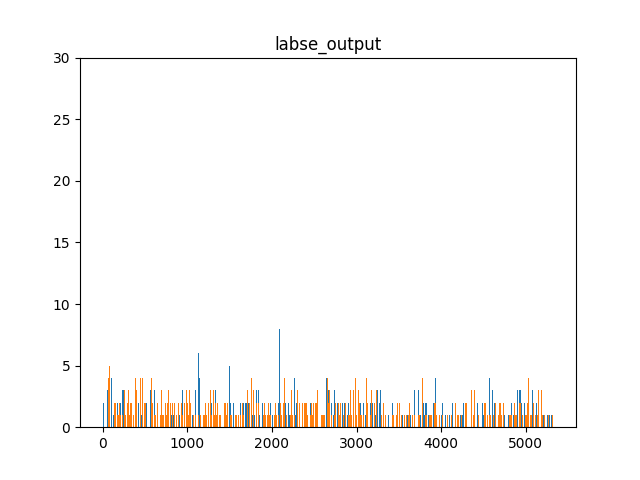
\includegraphics[width=0.8\linewidth]{figures/semantics/labse_output.png}
    \caption{Ilości reprezentacji przykładów jako pozytywne i negatywne dla modelu Labse w ramach zbioru \textit{Medical Speech, Transcription, and Intent}. Kolorem pomarańczowym oznaczono ilość zdań, dla których dany przykład jest przykładem negatywnym, niebieskim -- pozytywnym}
    \label{fig:latent:labseDistribution}
\end{figure}

\begin{figure}
    \centering
    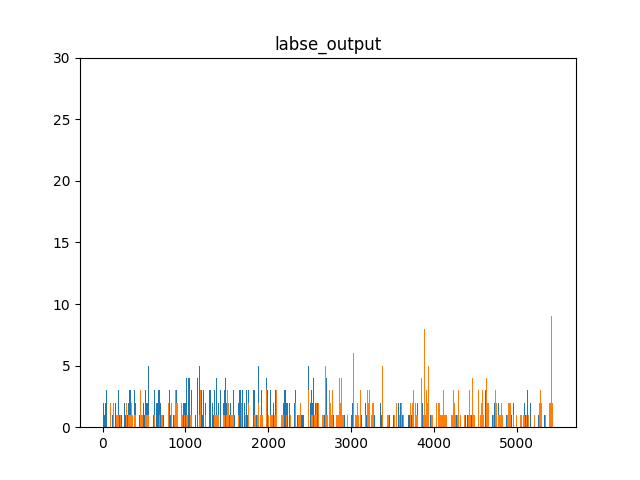
\includegraphics[width=0.8\linewidth]{figures/semantics/fleurs_labse_output.png}
    \caption{Ilości reprezentacji przykładów jako pozytywne i negatywne dla modelu Labse w ramach zbioru FLEURS. Kolorem pomarańczowym oznaczono ilość zdań, dla których dany przykład jest przykładem negatywnym, niebieskim -- pozytywnym}
    \label{fig:latent:labseDistributionFleurs}
\end{figure}

Rozkłady przykładów $x^n$ i $x^p$, dzięki zastosowaniu losowego wyboru były dosyć równomierne dla obu zbiorów danych, co przedstawiono na rysunkach \ref{fig:latent:labseDistribution} i \ref{fig:latent:labseDistributionFleurs}.

\subsubsection{Implementacja}
Eksperymenty zostały przeprowadzone z wykorzystaniem języka Python w wersji 3.12. Modele ASR i embeddingowe wraz z ich wagami zostały pobrane ze strony HuggingFace za pomocą bibliotek \textit{transformers} i \textit{sentence-transformers}. Do szybkiego obliczenia odległości między embeddingami wraz z wyłonieniem najbliższych i najdalszych embeddingów wykorzystaliśmy biblioteki \textit{Pytorch} i \textit{keOps}. Do obliczeń pomocniczych wykorzystaliśmy bibliotekę \textit{numpy}, natomiast do wizualicji -- \textit{matplotlib}. Eksperyment przeprowadzony został na serwerze obliczeniowym przy użyciu karty graficznej Nvidia RTX A5000.
\subsubsection{Analiza wyników}

\paragraph{Analiza enkodowania znaczenia semantycznego mowy}

Rozkłady wartości metryki $S(x_{emb,asr})$ (równanie \ref{eq:tripletDiff}) dla poszczególnych modeli ASR przedstawione są na wykresach zamieszczonych w sekcji Dodatki.

Tabela \ref{tab:latent:haniaCounts} przedstawia ilość przykładów w ramach zbioru danych \textit{Medical Speech, Transcription, and Intent}, dla których metryka $S(x_{emb,asr})$ przyjmowała wartości dodatnie, czyli tam, gdzie model ASR z powodzeniem uchwycił relacje semantyczne. Widać na niej wyraźną przewagę modelu SeamlessM4T, jak i dobre wyniki dla modeli Whisper i Hubert, które uchwyciły podobieństwo dla podobnie wysokiej liczby przykładów w ramach tego zbioru danych.

Tabela \ref{tab:latent:haniaDist} ilustruje z kolei parametry dopasowanego przez nas rozkładu Student-t dla zagregowanych różnic podobieństwa w ramach wszystkich modeli embeddingowych. Liczba stopni swobody $\nu$ odpowiedzialna jest za opisanie stabilności rozkładu w świetle obecności ogonów - im większa, tym bardziej stabilny jest rozkład. Wartości zbliżone do 2, jakie otrzymaliśmy dla modeli Data2Vec, Wav2Vec i Whisper wskazują na ich wysoką niestabilność w uchwyceniu relacji semantycznych. SeamlessM4T okazuje się najbardziej przewidywalnie zachowującym się modelem, dla którego $\nu = 6.4$, znacznie przewyższając drugi najwyżej plasujący się model HuBERT ($\nu = 3.6$). Znormalizowana lokalizacja ($\mu/\sigma$) pozwala nam na porównanie separacji pozytywnych i negatywnych przykładów między ewaluowanymi modelami ASR (MMD nie zachowuje skali pomiędzy modelami). Po raz kolejny, model SeamlessM4T wykazuje się najsilniejszą zdolnością rozróżniania przykładów pozytywnych i negatywnych ($\mu/\sigma = 0.91$). Modele HuBERT i Whisper osiągneły wyniki blisko dwukrotnie gorsze ($\mu/\sigma = 0.61$ i $\mu/\sigma = 0.54$), natomiast Data2Vec i Wav2Vec przejawiają podobnie niską zdolność dyskryminacji ($\mu/\sigma \approx 0.33$). Ostatnią z badanych metryk jest prawdopodobieństwo prawidłowego uchwycenia relacji między $x^a$, $x^n$ i $x^p$. Jest ona podobna do podejścia stricte ilościowego, lecz pozwala ona również analizować osiągi modelu w świetle dopasowanego przez nas rozkładu. Podobnie jak w porównaniu ilościowym, SeamlessM4T deklasuje resztę modeli, natomiast zarówno Whisper jak i HuBERT wykazują podobnie dobre wyniki. Warto zauważyć jednak, że HuBERT osiąga lepsze wyniki dla tej metryki ($P(neg > pos) = 71\%$) niż Whisper ($P(neg>pos) = 67.8\%$), wskazując na przewagę tego modelu, niewidoczną dla porównania ilościowego, która spowodowana jest prawdopodobnie większą stabilnością dopasowanego rozkładu.

\begin{table}[ht]
\centering
\caption{$S(x_{emb,asr}) > 0$ dla zbioru \textit{Medical Speech, Transcription, and Intent} (Ilość przykładów = 5327)}
\label{tab:latent:haniaCounts}
\begin{tabular}{lccc}
\toprule
\textbf{Model} & \textbf{Jina} & \textbf{LaBSE} & \textbf{SBERT} \\
\midrule
Wav2Vec  & 3352 & 3377 & 3472 \\
Data2Vec & 3290 & 3337 & 3375 \\
M4T  & \textbf{4375} & \textbf{4443} & \textbf{4413} \\
Whisper  & 3848 & 4006 & 3802 \\
HuBERT   & 3801 & 3971 & 3827 \\
\bottomrule
\end{tabular}
\end{table}

\begin{table}[t]
\centering
\begin{tabular}{lccc}
\hline
Model & Liczba stopni swobody ($\nu$) & Znormalizowana lokalizacja ($\mu/\sigma$) & $P(\text{neg} > \text{pos})$ \\
\hline
Data2Vec  & 2.1 & 0.32 & 61.1\% \\
Wav2Vec   & 2.3 & 0.35 & 62.1\% \\
M4T    & \textbf{6.4} & \textbf{0.98} & \textbf{81.8\%} \\
Whisper   & 1.9 & 0.54 & 67.8\% \\
HuBERT    & 3.6 & 0.61 & 71.0\% \\
\hline
\end{tabular}
\caption{Parametry rozkładów Student-$t$ dopasowanych do zagregowanych krzywych różnicy podobieństwa dla zbioru \textit{Medical Speech, Transcription, and Intent}}
\label{tab:latent:haniaDist}
\end{table}

Wyniki dla dwujęzycznej wersji zbioru Fleurs (język polski i angielski) zostały przedstawione dla modeli ASR wspierających oba z tych języków, reprezentujące trzy rodziny modeli - HuBERT (mHuBERT), Whisper i SeamlessM4T. Rozkłady dla tych modeli przedstawione zostały na rysunkach zamieszczonych w sekcji Dodatki. Tabele \ref{tab:latent:fleursCounts} i \ref{tab:latent:fleursDist} przedstawiają ilościowe porównanie wyników eksperymentu.

\begin{table}[ht]
\centering
\caption{$S(x_{emb,asr}) > 0$ dla zbioru \textit{Fleurs} (Ilość przykładów = 5443)}
\label{tab:latent:fleursCounts}
\begin{tabular}{lccc}
\toprule
\textbf{Model} & \textbf{Jina} & \textbf{LaBSE} & \textbf{SBERT} \\
\midrule
M4T  & \textbf{4256} & \textbf{4284} & \textbf{3911} \\
Whisper  & 3918 & 3895 & 3295 \\
HuBERT  & 3650 & 3721 & 3295 \\
mHuBERT   & 3296 & 3430 & 3288 \\
\bottomrule
\end{tabular}
\end{table}

\begin{table}[t]
\centering
\begin{tabular}{lccc}
\hline
Model & Liczba stopni swobody ($\nu$) & Znormalizowana lokalizacja ($\mu/\sigma$) & $P(\text{neg} > \text{pos})$ \\
\hline
M4T    & 6.8 & \textbf{0.72} & \textbf{75.3\%} \\
Whisper   & \textbf{10.4} & 0.49 & 68.3\% \\
HuBERT   & 8.3 & 0.40 & 64.9\% \\
mHuBERT    & 2.8 & 0.27 & 59.6\% \\
\hline
\end{tabular}
\caption{Parametry rozkładów Student-$t$ dopasowanych do zagregowanych krzywych różnicy podobieństwa dla zbioru \textit{Fleurs}}
\label{tab:latent:fleursDist}
\end{table}

Zarówno na podstawie Tabeli \ref{tab:latent:fleursCounts} jak i Tabeli \ref{tab:latent:fleursDist} zauważyć można dużą przewagę modelu M4T nad pozostałymi modelami. Zarówno umiejętność poprawnej separacji przykładów negatywnych i pozytywnych ($\mu/\sigma$ = 0.72), średnia ilość poprawnie przyporządkowanych przykładów ($E[n_\text{poz}] = 4150$), jak i prawdopodobieństwo poprawnego przyporządkowania przykładów ($P(\text{neg} > \text{poz}) = 75.3\%$) stawiają SeamlessM4T jako model najlepiej enkodujący semantykę wypowiedzi. Wyniki dla modelu Whisper również wskazują na enkodowanie przez niego znaczenia treści danych wejściowych, z gorszą zdolnością separacji przykładów ($\mu/\sigma$ = 0.49) i prawdopodobieństwem prawidłowego ich przyporządkowania ($P(\text{neg} > \text{poz}) = 68.3\%$), lecz z bardziej stabilnym rozkładem przypadków ($\nu = 10.4$) w porównaniu z SeamlessM4T ($\nu = 6.8$), co wskazuje na zadowalające zdolności modelu Whisper do reprezentacji semantyki danych wejściowych. Zdecydowanie najgorzej wypadł w tym porównaniu model mHuBERT, który z niskim prawdopodobieństwem poprawnie klasyfikował znaczenie danych wejściowych w świetale ich semantyki ($P(\text{neg} > \text{poz}) = 59.6\%$), osiągając wyniki niewiele większe niż wybór losowy i gorsze niż bazowy model HuBERT($P(\text{neg} > \text{poz}) = 64.5\%$). Możliwą przyczyną tak niskiego wyniku jest niska elastyczność modelu, stworzonego oryginalnie wyłącznie do transkrypcji mowy w języku angielskim, jak i mocy dekodera obecnego w pełnej propagacji w przód modelu. Kolejnym wyjaśnieniem jest zakłócenie oryginalnie silnej reprezentacji semantycznej w modelu angielskim (model HuBERT dla zbioru \textit{Medical Speech, Transcription, and Intent}, tabela \ref{tab:latent:haniaDist}) przez dotrenowanie na danych ze 146 kolejnych języków, przez które model o tak małej liczbie parametrów -- 94.4 miliona -- musiał enkodować tekst wejściowy w pewien bardziej skompresowany sposób, nie nadający się do interpretacji w świetle semantyki embeddingów. Hipotezę tę potwierdzają wyniki pracy \textit{Adapting multilingual speech representation model for a new, underresourced language through multilingual fine-tuning and continued pretraining}, w której autorzy zauważyli wyraźnie gorsze wyniki modelu dotrenowanego do transkrypcji języka Ainu na danych w języku angielskim (językowo bardzo różnym od Ainu) \cite{latentBreakMultilingual}. Wskazuje to na wysokie prawdopodobieństwo wystąpienia zjawiska zapominania (\textit{catastrophic forgetting}), analiza którego nie została umieszczona w oryginalnej pracy autorów mHuBERT-147 \cite{mhubert}.

Warto zwrócić uwagę na parametr $\nu$ opisujący stabilność rozkładu, który największa wartość przyjmuje dla modelu Whisper, w porównaniu do jego wartości dla zbioru \textit{Medical Speech, Transcription, and Intent} - dla zbioru \textit{Fleurs} modele o wiele lepiej radzą sobie z ekstremalnymi przypadkami odległości przykładów \textit{anchor}, \textit{pos} i \textit{neg}. Jest to najprawdopodobniej spowodowane kombinacją dwóch czynników -- sztucznej separacji przestrzeni embeddingowej między dwoma językami, która w mniejszym lub większym stopniu jest obecna w każdym z badanych modeli jak i szerszą domeną samego zbioru danych \textit{Fleurs}, który nie skupia się wyłącznie na tematycze medycznej.

%
% Cone
%
\paragraph{Analiza efektu stożka dla wybranych wielojęzycznych modeli ASR}

\begin{figure}
    \centering
    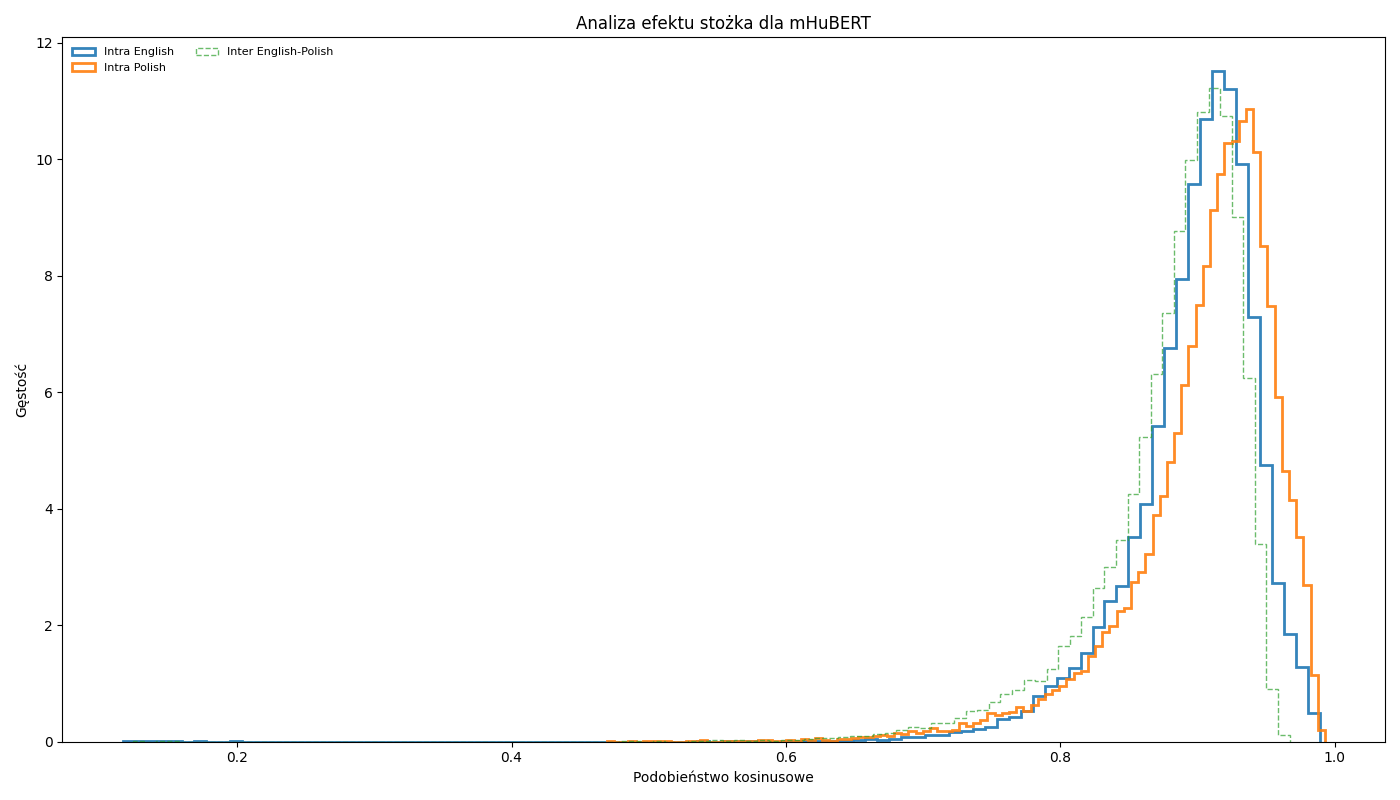
\includegraphics[width=0.8\linewidth]{figures/semantics/mhubert_cone.png}
    \caption{Gęstość podobieństwa kosinusowego z uwzględnieniem języków dla mHuBERT w ramach zbioru \textit{Fleurs}}
    \label{fig:latent:coneMHubert}
\end{figure}

\begin{figure}
    \centering
    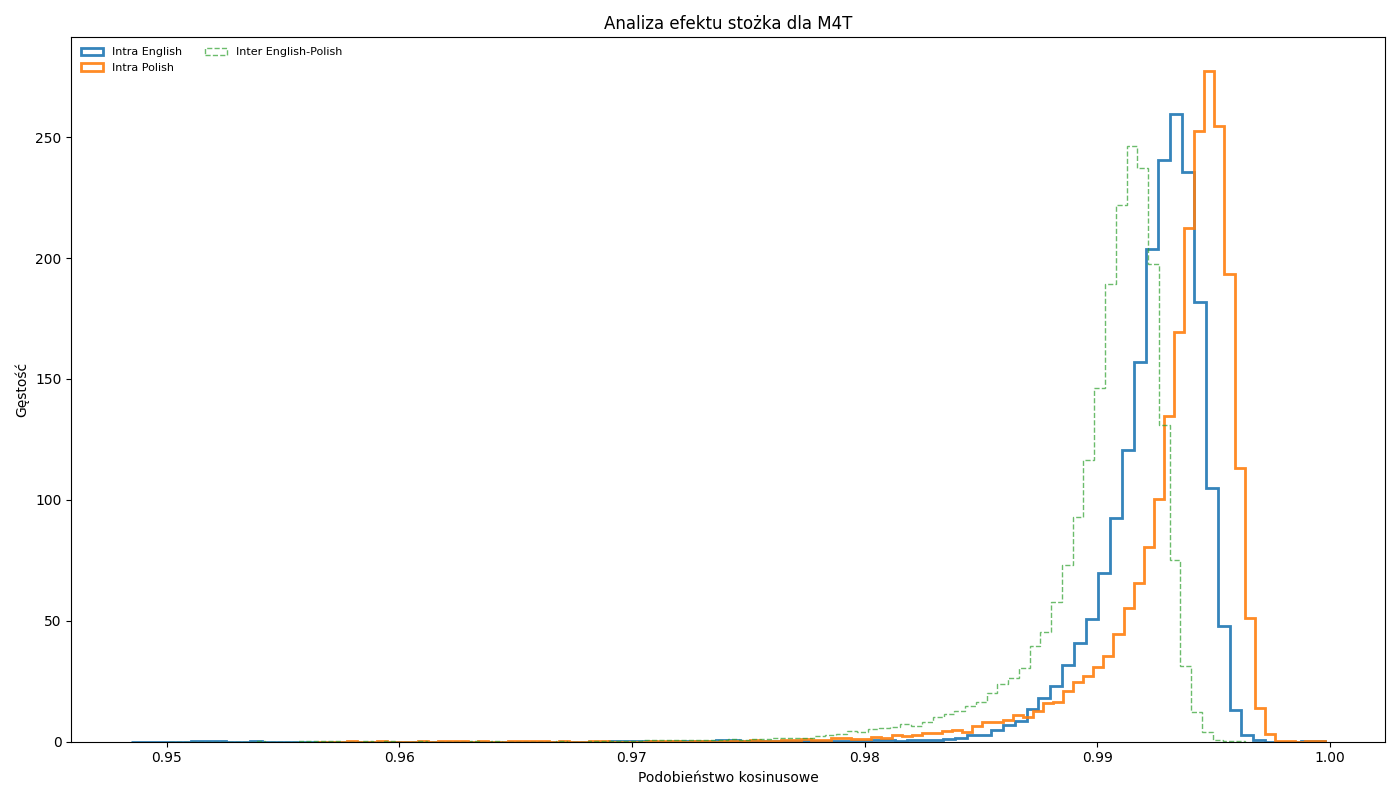
\includegraphics[width=0.8\linewidth]{figures/semantics/m4t_cone.png}
    \caption{Gęstość podobieństwa kosinusowego z uwzględnieniem języków dla M4T w ramach zbioru \textit{Fleurs}}
    \label{fig:latent:coneM4T}
\end{figure}

\begin{figure}
    \centering
    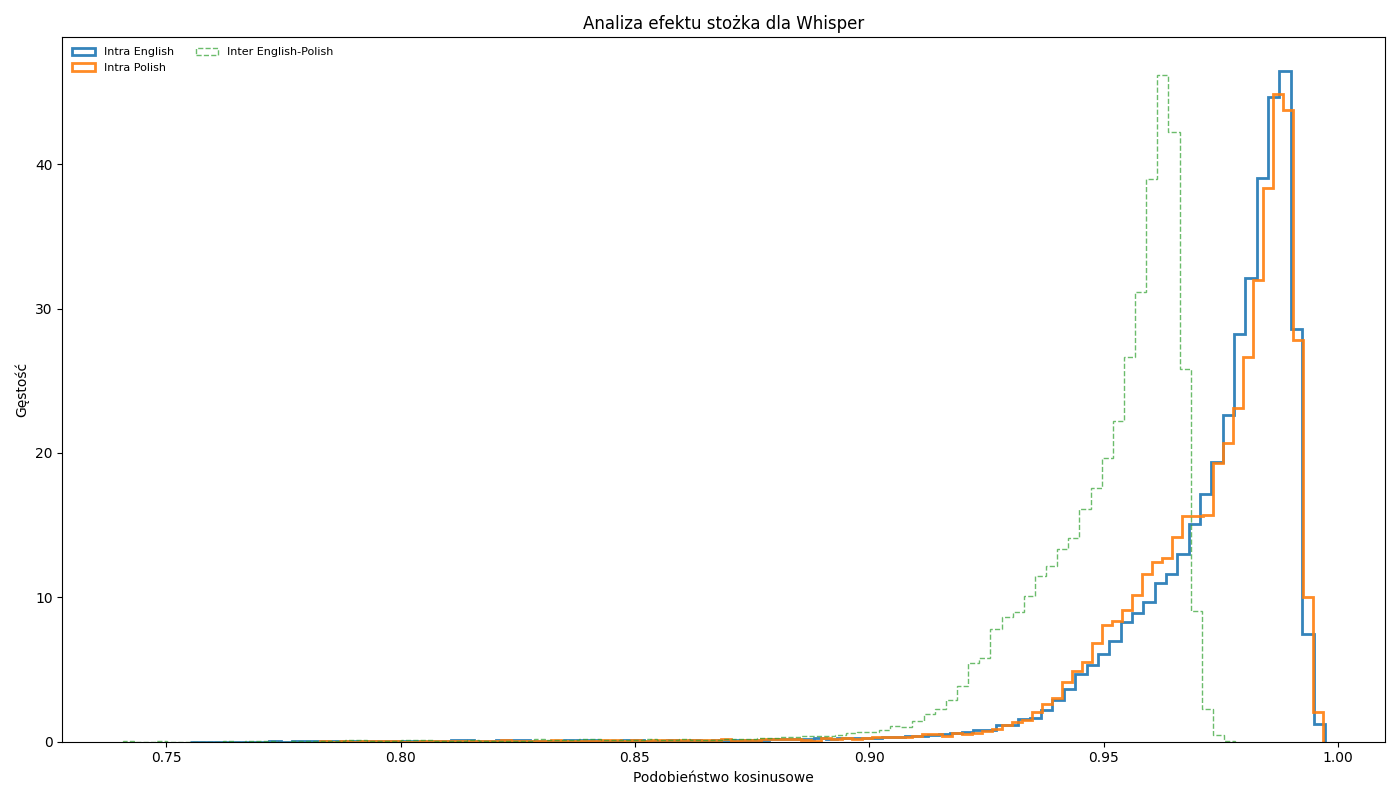
\includegraphics[width=0.8\linewidth]{figures/semantics/whisper_cone.png}
    \caption{Gęstość podobieństwa kosinusowego z uwzględnieniem języków dla Whisper w ramach zbioru \textit{Fleurs}}
    \label{fig:latent:coneWhisper}
\end{figure}

Wykresy gęstości podobieństwa kosinusowego dla zbioru \textit{Fleurs} w zależności od języków przedstawione zostały na rysunkach \ref{fig:latent:coneMHubert}, \ref{fig:latent:coneM4T} i \ref{fig:latent:coneWhisper}


Widoczny jest tutaj wyraźnie fenomen stożka, zgodny z zależnością zaobserwowaną w pracy \textit{How Contextual are Contextualized Word Representations? Comparing the Geometry of BERT, ELMo, and GPT-2 Embeddings}, w której autor zauważył wzrost anizotropi przestrzeni ukrytych modeli językowych wraz ze wzrostem ilości warstw \cite{cone} -- wraz ze wzrostem liczby parametrów i warstw, reprezentacje latentne zajmują coraz to mniejszy fragment przestrzeni (rozkład dla mHuBERT -- 94.4 miliona parametrów [rysunek \ref{fig:latent:coneMHubert}] a ten sam rozkład dla SeamlessM4T -- 2 miliardy parametrów [rysunek \ref{fig:latent:coneM4T}]). W celu stwierdzenia czy reprezentacje mowy wymawianej w różnych językach tworzą osobne klastry w przestrzeni embeddingowej należy spojrzeć na odległość między wykresami gęstości dla podobieństw kosinusowych wewnątrz języków i między językami. Modele mHuBERT i SeamlessM4T wydają się enkodować informacje agnostycznie od języka, z separacją między grupami językowymi będącą wyraźnie najmniejszą dla pierwszego modelu (częściowe pokrycie i niewielkie przesunięcie gęstości między grupami a wewnątrz grup na rysunkach \ref{fig:latent:coneMHubert} i \ref{fig:latent:coneM4T}). Model Whisper wykazuje dosyć dużą separację między grupami językowymi w ramach reprezentacji latentnych (rysunek \ref{fig:latent:coneWhisper}). Właściwość ta może prowadzić do mniej dokładnego wyszukiwania informacji między językami polskim i angielskim, a także do gorszego transferu wiedzy pozyskanej w ramach treningu na specjalistycznych zbiorach w języku angielskim do analogicznej wiedzy w języku polskim.

\begin{figure}
    \centering
    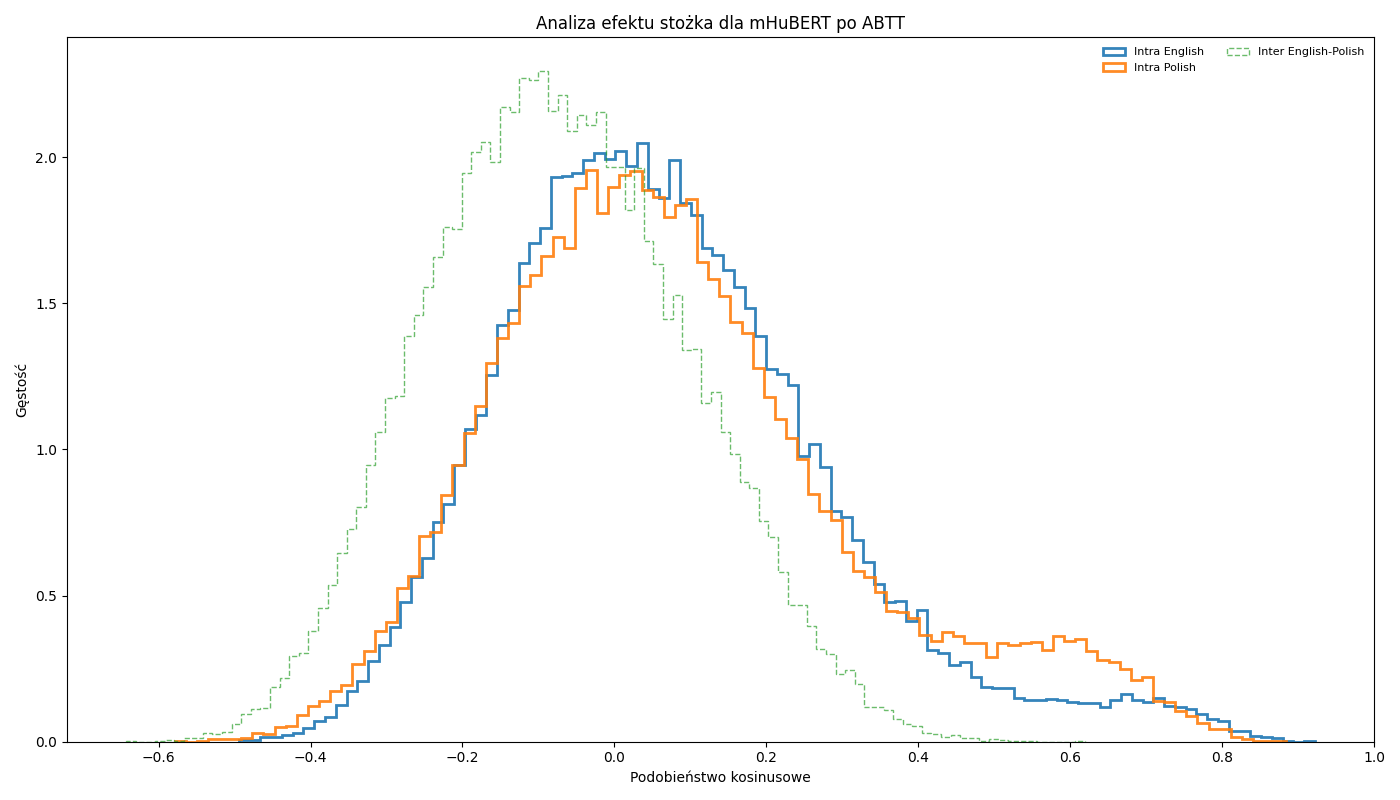
\includegraphics[width=0.8\linewidth]{figures/semantics/mhubert_cone_abtt.png}
    \caption{Gęstość podobieństwa kosinusowego z uwzględnieniem języków dla MHuBERT w ramach zbioru \textit{Fleurs} po transformacji ABTT}
    \label{fig:latent:coneMhubertAbtt}
\end{figure}

\begin{figure}
    \centering
    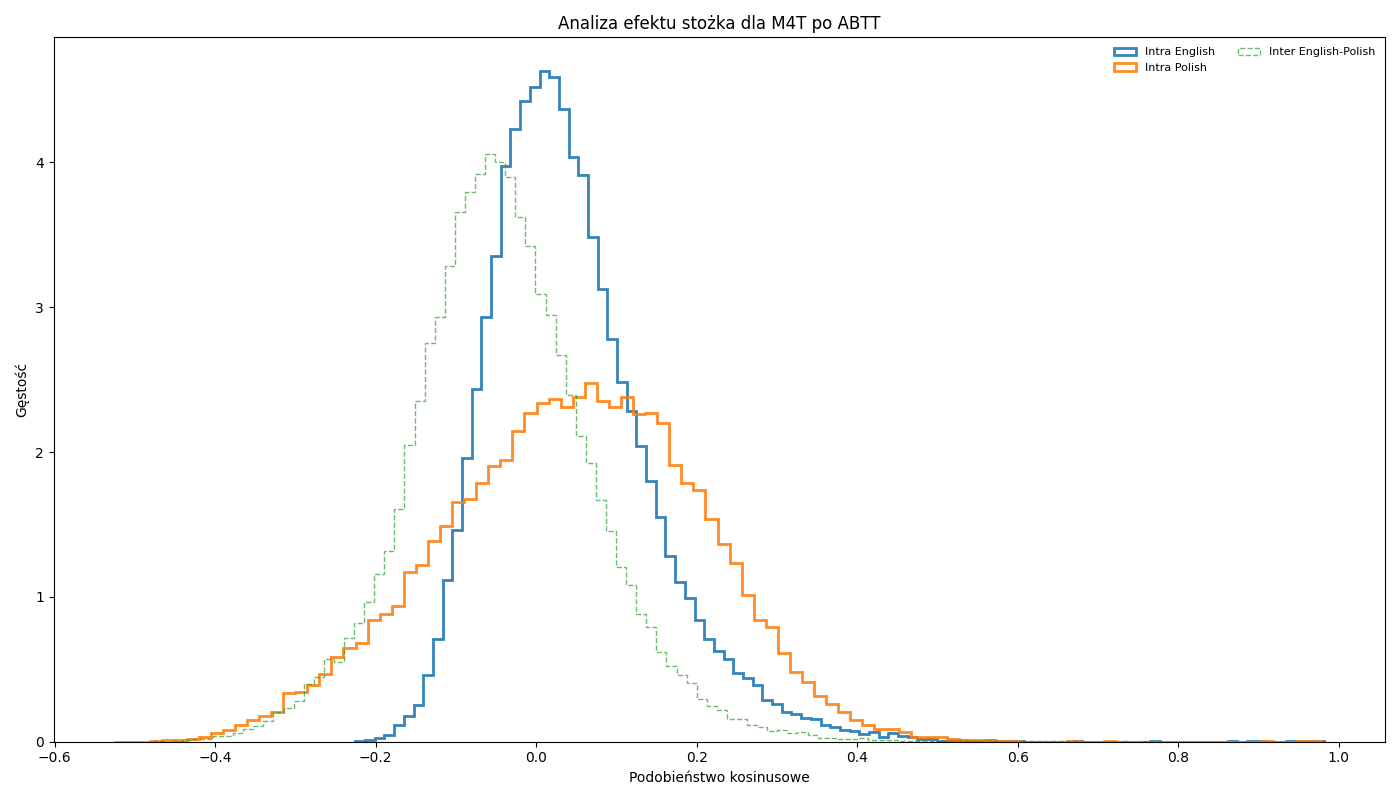
\includegraphics[width=0.8\linewidth]{figures/semantics/m4t_cone_abtt.png}
    \caption{Gęstość podobieństwa kosinusowego z uwzględnieniem języków dla M4T w ramach zbioru \textit{Fleurs} po transformacji ABTT}
    \label{fig:latent:coneM4TAbtt}
\end{figure}

\begin{figure}
    \centering
    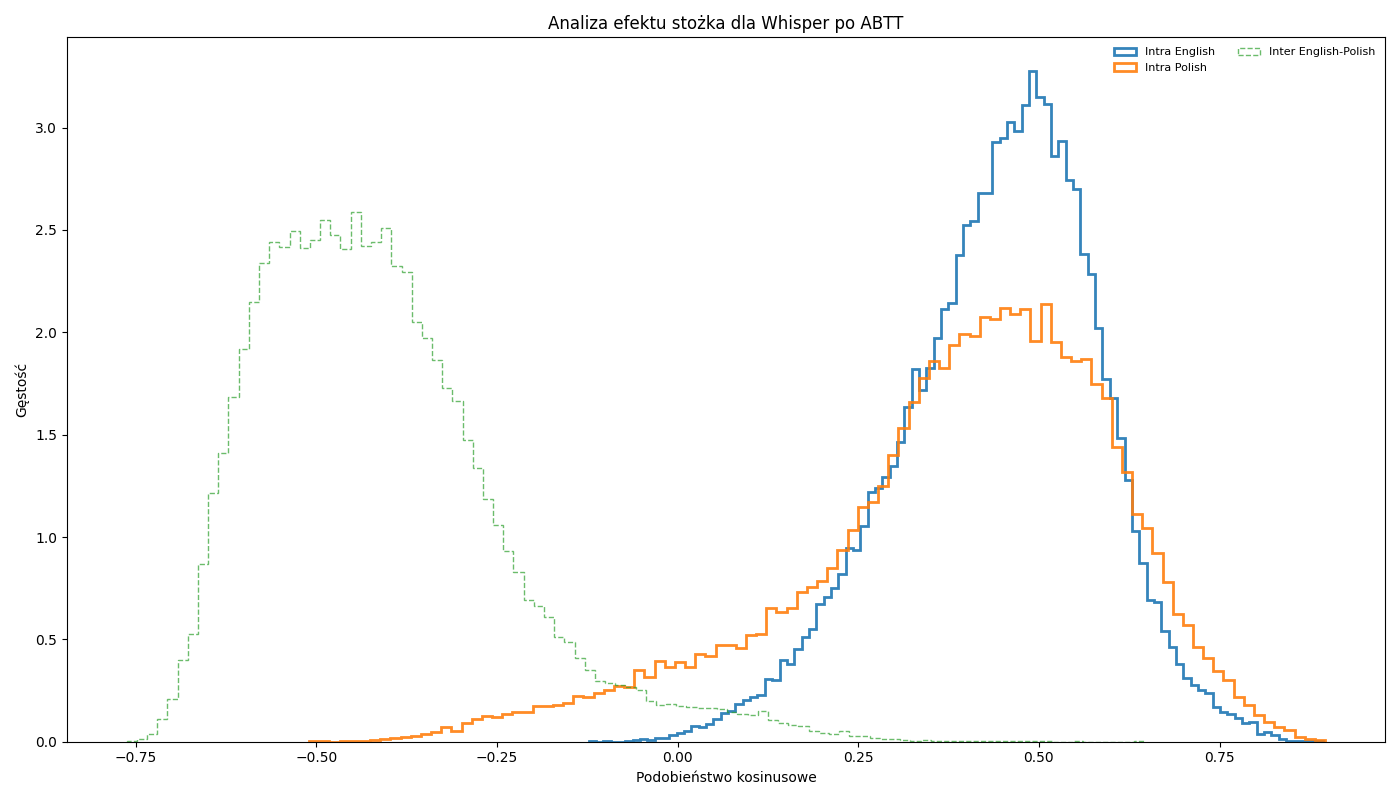
\includegraphics[width=0.8\linewidth]{figures/semantics/whisper_cone_abtt.png}
    \caption{Gęstość podobieństwa kosinusowego z uwzględnieniem języków dla Whisper w ramach zbioru \textit{Fleurs} po transformacji ABTT}
    \label{fig:latent:coneWhisperAbtt}
\end{figure}

Rysunki \ref{fig:latent:coneMhubertAbtt}, \ref{fig:latent:coneM4TAbtt} i \ref{fig:latent:coneWhisperAbtt} przedstawiają rozkłady gęstości podobieństwa kosinusowego między embeddingami po przekształceniu \textit{All But the Top}. Dla wszystkich modeli, badane reprezentacje latentne zajęły większą część dostępnej przestrzeni. Jest to spowodowane usunięciem pierwszej głównej składowej po analizie PCA, dzięki czemu pewne wspólne informacje przechowywane przez reprezentacje latentne zostały odrzucone, pozostawiając wyłącznie cechy własne charakteryzujące dane wejściowe. Model mHuBERT (rysunek \ref{fig:latent:coneMhubertAbtt}) zachował prawie identyczne rozkłady w ramach grup językowych, z gęstością podobieństwa lekko przesuniętą. Wskazuje to na większą separację grup językowych niż w ramach danych nieprzetworzonych (rysunek \ref{fig:latent:coneMHubert}). Może być to spowodowane tendencją modelu do enkodowania informacji dotyczących języka, w niewielkim stopniu, na przykład informacji prozodycznych. Seamless M4T wykazuje się podobną charakterystyką co do przesunięcia podobieństwa między grupami, które było obecne również dla danych nieprzetworzonych (rysunki \ref{fig:latent:coneM4TAbtt} i \ref{fig:latent:coneM4T}). Warto zwrócić uwagę na różnicę rozkładów wewnątrz grup językowych -- embeddingi dla języka polskiego zajmują o wiele większą część przestrzeni niż embeddingi dla języka angielskiego. Naszą hipotezą jest obecność pewnego meta-języka opisującego dane dla modelu M4T, który podobny jest najbardziej do języka angielskiego. O ile autorzy modelu nie podali dokładnego balansu danych między różnymi językami w ramach danych treningowych modelu \cite{m4t}, można przypuszczać dominację danych w języku angielskim, stąd też bardziej dokładne reprezentacje danych w języku angielskim. Charakterystyka modelu Whisper (rysunek \ref{fig:latent:coneWhisperAbtt}) zaobserwowana dla danych nieprzetworzonych (rysunek \ref{fig:latent:coneWhisper}) została potwierdzona przez rozkłady dla embeddingów po przetworzeniu \textit{All But the Top}. Widoczna jest o wiele bardziej wyraźna separacja na pewne klastry reprezentujące języki polski i angielski. Jest to najprawdopodobniej spowodowane charakterystyką treningu, w ramach której funkcja straty nie wymusza w jakikolwiek sposób współdzielenia przestrzeni latentnej przez dane z różnych języków, dane treningowe dla transkrypcji precyzują język wypowiedzi \cite{whisper}.

\begin{figure}
    \centering
    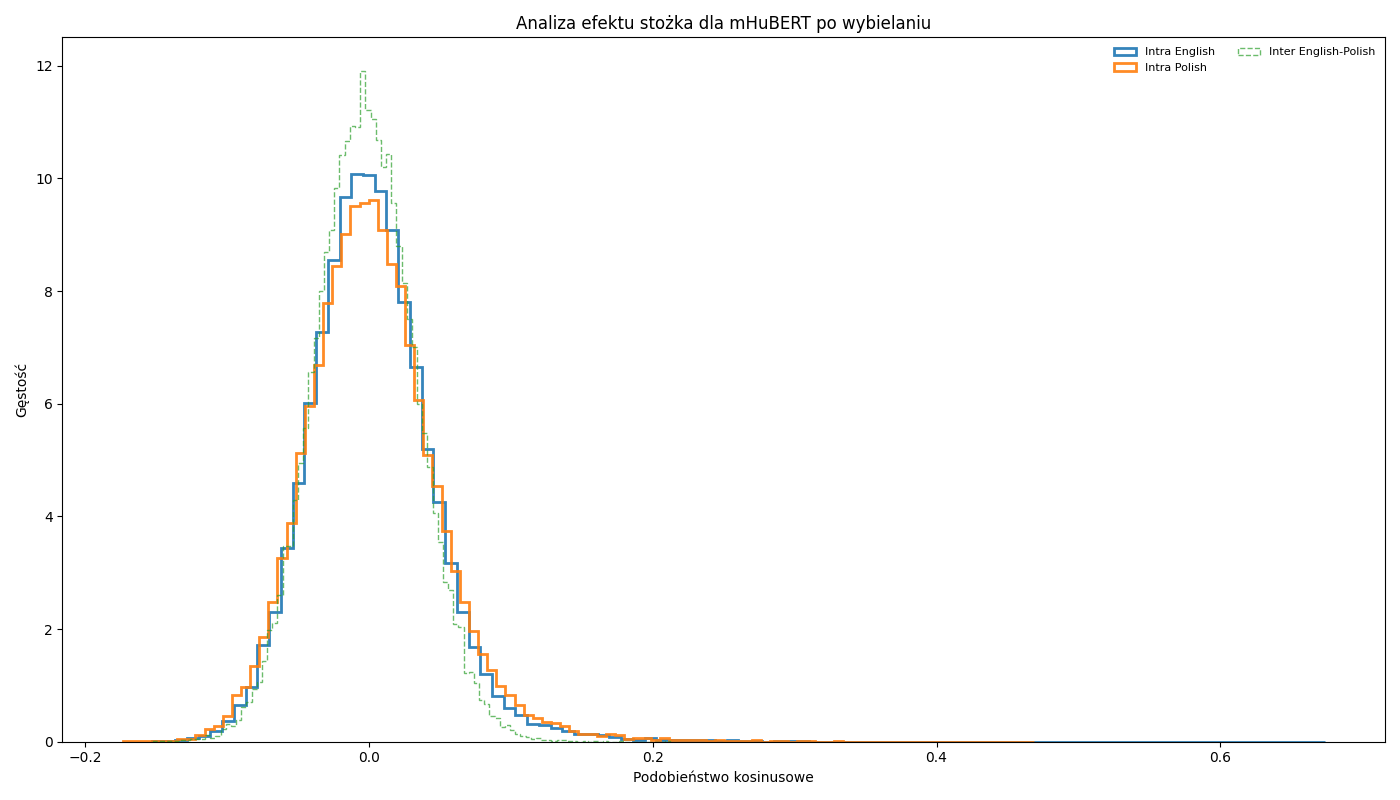
\includegraphics[width=0.8\linewidth]{figures/semantics/mhubert_cone_whitened.png}
    \caption{Gęstość podobieństwa kosinusowego z uwzględnieniem języków dla MHuBERT w ramach zbioru \textit{Fleurs} po wybielaniu}
    \label{fig:latent:coneMhubertWhitened}
\end{figure}

\begin{figure}
    \centering
    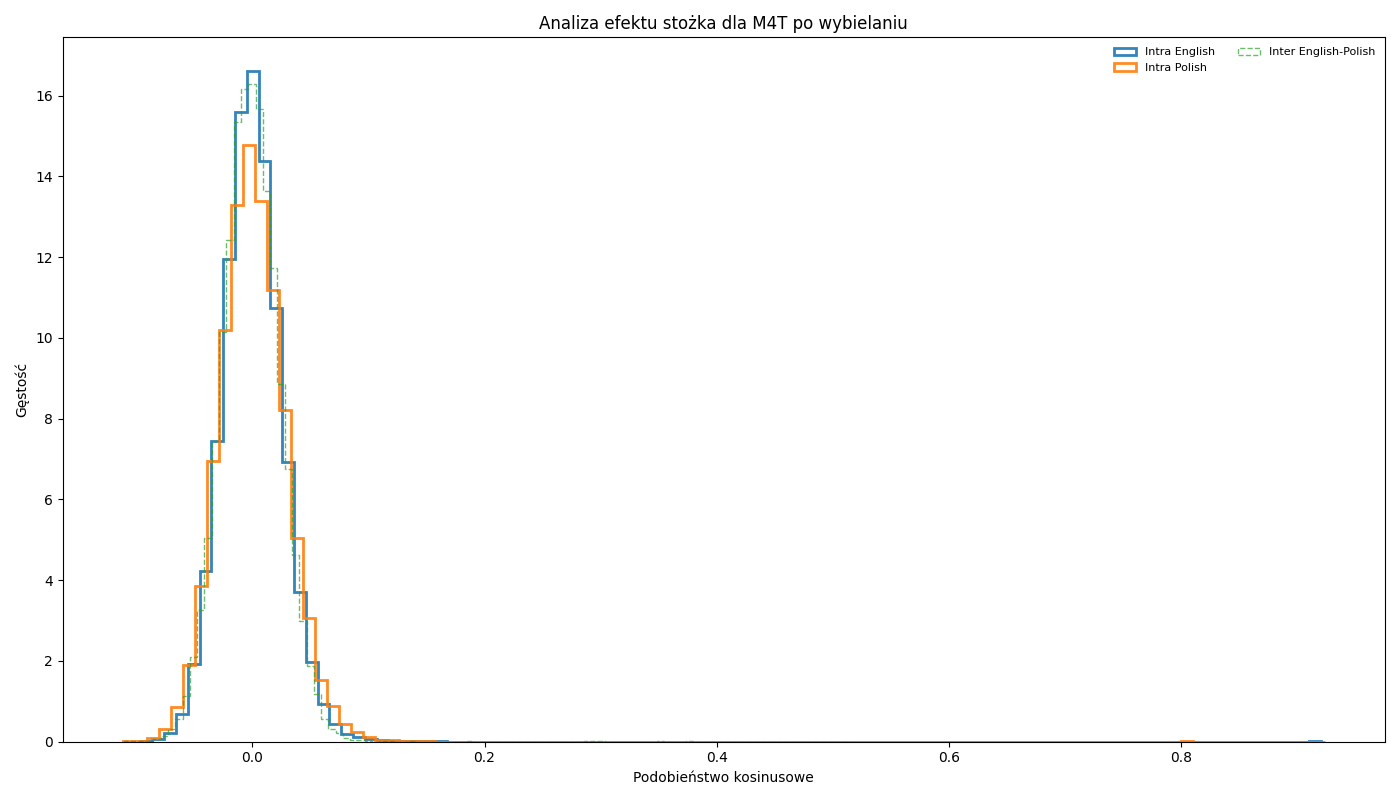
\includegraphics[width=0.8\linewidth]{figures/semantics/m4t_cone_wnitened.png}
    \caption{Gęstość podobieństwa kosinusowego z uwzględnieniem języków dla M4T w ramach zbioru \textit{Fleurs} po wybielaniu}
    \label{fig:latent:coneM4TWhitened}
\end{figure}

\begin{figure}
    \centering
    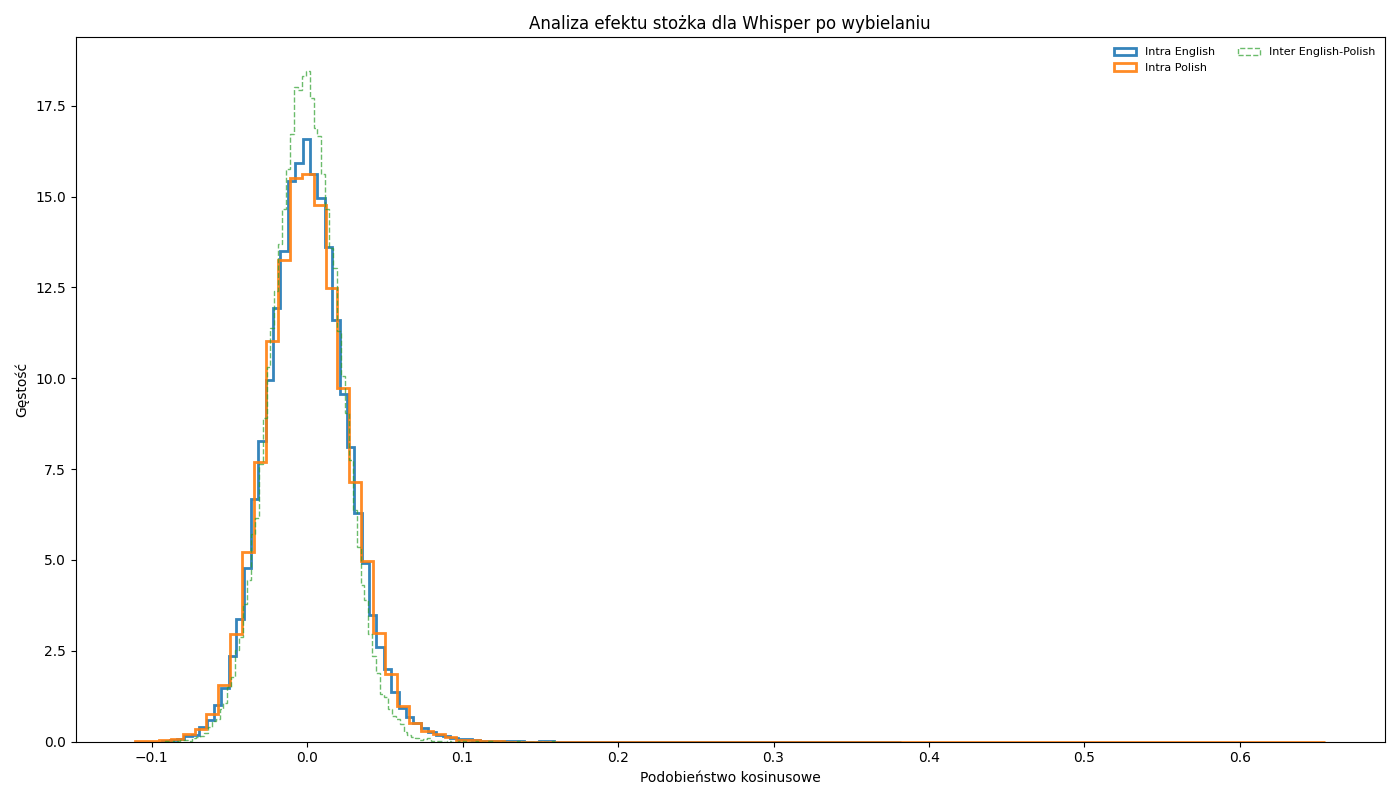
\includegraphics[width=0.8\linewidth]{figures/semantics/whisper_cone_wnitened.png}
    \caption{Gęstość podobieństwa kosinusowego z uwzględnieniem języków dla Whisper w ramach zbioru \textit{Fleurs} po wybielaniu}
    \label{fig:latent:coneWhisperWhitened}
\end{figure}

Rysunki \ref{fig:latent:coneMhubertWhitened}, \ref{fig:latent:coneM4TWhitened} i \ref{fig:latent:coneWhisperWhitened} przedstawiają rozkłady podobieństwa kosinusowego po przeprowadzeniu wybielania (\textit{whitening}). Dzięki dekorelacji danych w ramach tego procesu, widoczna jest tutaj bliska idealnej umiejętność łączenia języków w jedną grupę, co prowadzi do dobrego transferu wiedzy między językami. Jednakże, w porównaniu z rozkładami dla przetwarzania ABTT, widoczne jest pewne zawężenie przestrzeni embeddingowej -- efekt stożka jest bardziej widoczny. Mimo tego, w świetle reprezentacji bazowych, embeddingi zajmują o wiele większy odsetek dostępnej przestrzeni.

Podsumowując, zabieg ABTT zdecydowanie poprawił ogólny rozkład embeddingów w przestrzeni, nie do końca redukując (a dla modelu Whisper pogłębiając) separację między reprezentacjami różnych języków. Wybielanie pozwoliło również na redukcję efektu stożka, tym samym dekorelując embeddingi w świetle języka, potencjalnie poprawiając transfer wiedzy w ramach treningu na danych w języku angielskim. Analiza ta wykazała poprawność wykorzystania postprocsessingu w świetle niwelowania anizotropi reprezentacji ukrytych dla modeli ASR.

\paragraph{Analiza wpływu przetwarzania embeddingów na zachowanie semantyki}
Oprócz modeli poddanych analizie w ramach badania efektu stożka, tj. Whisper, mHuBERT i SeamlessM4T, w tym eksperymencie uwzględniliśmy róznież bazowy model HuBERT, który wykazywał dobre wyniki w ramach zbiorów \textit{Medical Speech, Transcription, and Intent} i \textit{Fleurs}.

Tabele \ref{tab:latent:cosCompNu}, \ref{tab:latent:cosineComparisonSeparability} i \ref{tab:latent:cosComparisonProbability} ilustrują porównanie parametrów dopasowanych rozkładów Student-t między analizą za pomocą metryki MMD i podobieństwa kosinusowego, natomiast rysunki przedstawiające te rozkłady umieszczone zostały w sekcji Dodatki.
\begin{table}[h]
\centering
\begin{tabular}{lccc}
\toprule
Model & MMD ($\nu$) & Podobieństwo kosinusowe ($\nu$) & Zmiana (\%) \\
\midrule
M4T     & 6.8  & 4.7  & -30.9 \\
Whisper & \textbf{10.4} & 7.6  & -26.9 \\
HuBERT  & 8.3  & \textbf{24.8} & \textbf{+198.8} \\
mHuBERT & 2.8  & 4.2  & +50.0 \\
\bottomrule
\end{tabular}
\caption{Porównanie parametru $\nu$ dla rozkładów MMD i podobieństwa kosinusowego.}
\label{tab:latent:cosCompNu}
\end{table}

\begin{table}[h]
\centering
\begin{tabular}{lccc}
\toprule
Model & MMD ($\mu/\sigma$) & Podobieństwo kosinusowe ($\mu/\sigma$) & Zmiana (\%) \\
\midrule
M4T     & \textbf{0.72} & \textbf{1.11} & \textbf{+54.2} \\
Whisper & 0.49 & 0.52 & +6.1 \\
HuBERT  & 0.40 & 0.31 & -22.5 \\
mHuBERT & 0.27 & 0.32 & +18.5 \\
\bottomrule
\end{tabular}
\caption{Porównanie parametru $\mu/\sigma$ dla rozkładów MMD i podobieństwa kosinusowego.}
\label{tab:latent:cosineComparisonSeparability}
\end{table}

\begin{table}[h]
\centering
\begin{tabular}{lccc}
\toprule
Model & MMD ($P$) & Podobieństwo kosinusowe ($P$) & Zmiana (\%) \\
\midrule
M4T     & \textbf{75.3} & \textbf{83.9} & \textbf{+11.4} \\
Whisper & 68.3 & 69.2 & +1.3 \\
HuBERT  & 64.9 & 62.1 & -4.3 \\
mHuBERT & 59.6 & 61.9 & +3.9 \\
\bottomrule
\end{tabular}
\caption{Porównanie prawdopodobieństw poprawnego uchwycenia relacji między przykładami bazowym, pozytywnym i negatywnym (MMD vs podobieństwo kosinusowe).}
\label{tab:latent:cosComparisonProbability}
\end{table}

W tabeli \ref{tab:latent:cosCompNu} widoczna jest stabilizacja rozkładu dla modeli z rodziny BERT (zmiana o $198.8\%$ i $50.0\%$ dla HuBERT i mHuBERT), z destabilizacją dla dwóch pozostałych modeli. Tabele \ref{tab:latent:cosineComparisonSeparability} i \ref{tab:latent:cosComparisonProbability} wykazują widoczny trend poprawy zarówno zdolności separacji, jak i ogólnej zdolności dyskryminacji pozytywnych i negatywnych przykładów dla SeamlessM4T i Whisper, z większym wzrostem metryk dla pierwszego z nich (wzrost o $54.2\%$ w znormalizowanej lokalizacji, $11.4\%$ w prawdopodobieństwie poprawnego uchwycenia relacji). Jest to prawdopodobnie spowodowane uniwersalnością enkodera SeamlessM4T, gdzie cały model wspiera modalności tekstu i mowy, przez co relacje czasowe muszą być zunifikowane w ramach tokenów tekstu i mowy. Whisper natomiast wykorzystuje najprawdopodobniej pewne zależności czasowe samej mowy, przez co usunięcie domeny czasu wiąże się z większą stratą informacji niż dla SeamlessM4T. Podobna właściwość modeli z rodziny BERT może stanowić również wyjaśnienie ich zachowania po usunięciu informacji z domeny czasu - zarówno mHuBERT, jak i HuBERT wykazują prawie identyczne właściwości względem separacji i zdolności poprawnej dyskryminacji rozkładu. Możliwe jest, że uśrednianie tokenów prowadzi do degradacji przestrzeni do prawie identycznej reprezentacji dla obu modeli.



Tabele \ref{tab:latent:compNu}, \ref{tab:latent:compLoc} i \ref{tab:latent:compProb} przedstawiają porównanie parametrów rozkładów dla embeddingów poddanych przetwarzaniu ABTT i wybielaniu. Wykresy przedstawiające te rozkłady zamieszczone zostały w sekcji Dodatki. Tabela \ref{tab:latent:processingCounts} przedstawia analizę ilościową poprawnie sklasyfikowanych przypadków. Ilości zostały uśrednione w ramach trzech różnych modeli embeddingowych.

\begin{table}[h]
\centering
\begin{tabular}{lccc}
\toprule
Model &
Podobieństwo kosinusowe &
ABTT &
Wybielanie \\
\midrule
M4T     & 4.7  & $1.96\times10^{10}$ & 0.8 \\
Whisper & 7.6  & $1.27\times10^{11}$ & 0.9 \\
HuBERT  & \textbf{24.8} & \textbf{$5.62\times10^{11}$} & 0.8 \\
mHuBERT & 4.2  & 5.2                 & \textbf{1.0} \\
\bottomrule
\end{tabular}
\caption{Porównanie parametru $\nu$ dla metod ABTT i wybielania względem bazowego podobieństwa kosinusowego.}
\label{tab:latent:compNu}
\end{table}

\begin{table}[h]
\centering
\begin{tabular}{lccccc}
\toprule
Model &
\multicolumn{1}{c}{Podobieństwo kosinusowe} &
\multicolumn{1}{c}{ABTT} &
\multicolumn{1}{c}{Zmiana (\%)} &
\multicolumn{1}{c}{Wybielanie} &
\multicolumn{1}{c}{Zmiana (\%)} \\
\midrule
M4T     & \textbf{1.11} & \textbf{1.41} & \textbf{+27.0} & 0.85 & -23.4 \\
Whisper & 0.52 & 0.44 & -15.4 & \textbf{0.95} & \textbf{+82.7} \\
HuBERT  & 0.31 & 0.34 & +9.7  & 0.52 & +67.7 \\
mHuBERT & 0.32 & 0.36 & +12.5 & 0.47 & +46.9 \\
\bottomrule
\end{tabular}
\caption{Porównanie parametru $\mu/\sigma$ dla metod ABTT i wybielania względem bazowego podobieństwa kosinusowego.}
\label{tab:latent:compLoc}
\end{table}

\begin{table}[h]
\centering
\begin{tabular}{lccccc}
\toprule
Model &
\multicolumn{1}{c}{Podobieństwo kosinusowe} &
\multicolumn{1}{c}{ABTT} &
\multicolumn{1}{c}{Zmiana (\%)} &
\multicolumn{1}{c}{Wybielanie} &
\multicolumn{1}{c}{Zmiana (\%)} \\
\midrule
M4T     & \textbf{83.9} & \textbf{92.1} & \textbf{+9.8} & 71.4 & -14.9 \\
Whisper & 69.2 & 67.1 & -3.0 & \textbf{73.1} & \textbf{+5.6} \\
HuBERT  & 62.1 & 63.3 & +1.9 & 64.5 & +3.9 \\
mHuBERT & 61.9 & 63.4 & +2.4 & 64.0 & +3.4 \\
\bottomrule
\end{tabular}
\caption{Porównanie prawdopodobieństwa poprawnego uchwycenia relacji między przykładami bazowym, pozytywnym i negatywnym dla metod ABTT i wybielania względem bazowego podobieństwa kosinusowego.}
\label{tab:latent:compProb}
\end{table}

\begin{table}[h]
\centering
\begin{tabular}{lccccc}
\toprule
Model &
Podobieństwo kosinusowe &
ABTT  &
Zmiana (\%) &
Wybielanie &
Zmiana (\%) \\
\midrule
M4T
& \textbf{4609} & \textbf{5131} & \textbf{+11.3} & \textbf{4915} & +6.6 \\
Whisper
& 3757 & 3816 & +1.6  & 4539 & \textbf{+20.8} \\
HuBERT
& 3474 & 3433 & -1.2  & 3951 & +13.7 \\
mHuBERT
& 3362 & 3402 & +1.2  & 3798 & +12.9 \\
\bottomrule
\end{tabular}
\caption{Średnia liczba poprawnych przypadków dla różnych embeddingów (Jina, LaBSE, SBERT) oraz względna poprawa metod ABTT i wybielania względem przypadku bazowego.}
\label{tab:latent:processingCounts}
\end{table}

Analizując Tabelę \ref{tab:latent:compNu}, zauważyć można popwawę stabilności rozkładu dla embeddingów poddanych przetwarzaniu ABTT dla wszystkich modeli. Jedynie mHuBERT nie osiągnął rozkładu praktycznie normalnego, lecz nadal cechuje się poprawą stabilności. Wybielanie doprowadziło z kolei do pewnej degradacji stabilności, uniwersalnie destabilizując wszytkie ewaluowane modele. Tak drastyczna różnica wynika zapewne z natury tych dwóch metod przetwarzania. O ile ABTT dokonuje wyłącznie projekcji do przestrzeni ortogonalnej do przestrzeni oryginalnej, o tyle wybielania prowadzi do rotacji i skalowania przestrzeni, mając o wiele większy wpływ na geometrię porównywanej przestrzeni, powodując odsunięcie się od rozkładu normalnego. Tabele \ref{tab:latent:compLoc} i \ref{tab:latent:compProb} pokazują zdolność separacji i prawdopodobieństwo poprawnego uchwycenia relacji przez modele. W modelach z rodziny HuBERT widoczna jest drastyczna poprawa zdolności separacji dla embeddingów poddanych wybielaniu ($67.7\%$ dla HuBERT, $46.9\%$ dla mHuBERT), jak i mniejsza, lecz zauważalna poprawa prawdopodobieństwa poprawnego uchwycenia badanej relacji ($3.9\%$ i $3.4\%$). Bardziej agresywna zmiana przestrzeni reprezentacji ukrytych poprawiła działanie tych modeli bardziej niż przekształcenie \textit{All But the Top}, które tylko nieznacznie poprawiło prawdopodobieństwo poprawnego przyporządkowania podobieństw przykładów. Mimo tego, modele te nie osiągnęły wyników większych niż wyniki bazowe dla modeli Whisper i SeamlessM4T. Dla tych dwóch modeli widoczna jest zgoła inna zależność i bardziej drastyczny wpływ doboru metody postprocessingu. SeamlessM4T poprawił swoje metryki o $27.0\%$ i $9.8\%$ dla ABTT, notując spadek dla bardziej agresywnej metody wybielania. Potencjalnym powodem są wysoka zdolność klasyfikacji semantycznej dla bazowego przypadku i zbyt duża modyfikacja geometrii przestrzeni po wykorzystaniu rotacji i skalowania, gdzie w przypadku ABTT informacje semantyczne nie są niszczone i poprawiana jest jedynie izotropia przestrzeni. Dla modelu Whisper ma miejsce zjawisko odwrotne -- to właśnie wybielanie poprawia wyniki modelu, a ABTT je redukuje. Negatywny wpływ metody \textit{All But the Top} powiązany może być z zachowaniem modelu w świetle efektu stożka przedstawionym na rysunku \ref{fig:latent:coneWhisperAbtt}, na którym wyraźnie widoczna jest separacja grup językowych, większa niż w przypadku nieprzetworzonych danych (rysunek \ref{fig:latent:coneWhisper}). Po wybielaniu modelu (rysunek \ref{fig:latent:coneWhisperWhitened}), w przestrzeni nie zauważono widocznych klastrów, co jest najbardziej prawdopodobnym powodem wzrostu badanych metryk. Jednakże, należy zauważyć wyraźną przewagę SeamlessM4T nad pozostałymi modelami, co potwierdza analiza ilościowa w tabeli \ref{tab:latent:processingCounts}. Nawet w ramach wybielania, które skutkuje spadkiem prawdopodobieństwa poprawnego uchwycenia relacji semantycznej o $14.9\%$, model ten poprawnie przyporządkował dane pod względem semantycznym większą ilość razy niż wszystkie inne badane modele.


\subsection{Podsumowanie i wnioski}
Wszystkie przeprowadzone przez nas eksperymenty wyraźnie wskazują na przewagę dwóch modeli ASR pod względem kodowania znaczenia semantycznego mowy -- SeamlessM4T i Whisper, dla których wyniki eksperymentów wskazują na kodowanie silnie nacechowanych semantycznie reprezentacji ukrytych. Pomimo potencjalnie bardziej stabilnego zachowania modeli z rodziny HuBERT, analiza ilościowa, jak i całościowa analiza parametrów dopasowanych rozkładów pokazały, że modele te nie są w stanie dorównać większym modelom w ramach wykorzystania ich jako enkoderów semantycznych cech mowy. Ponadto, wyniki wykazują pewną degradację semantyczności reprezentacji, nawet w ramach porównania na zbiorze wielojęzycznym, dla modelu mHuBERT w porównaniu z bazowym modelem HuBERT. Badając metody przetwarzania embeddingów, \textit{All But the Top} i wybielanie oparte na PCA, zauważyliśmy potencjalną poprawę reprezentacji, w szczególności dla modelów o wysokiej anizotropii przestrzeni, tj. SeamlessM4T i Whisper. Zmiany te jednak nadal nie podnoszą wyników mHuBERT i HuBERT na tyle, aby przewyższyć bazowe osiągi dwóch pozostałych modeli -- oznacza to, że dobór modelu ASR ma większe znaczenie niż dobór odpowiedniej metody przetwarzania embeddingów. Pokazaliśmy również poprawę reprezentacji względem grupowania reprezentacji danych wejściowych w języku polskim i angielskim, co umożliwi potencjalnie lepszy transfer wiedzy w ramach treningu na danych w obu tych językach.

Mając na uwadzę powyższe odkrycia, naturalnym wyborem do dalszej pracy nad modelami z rodziny speech-to-retrieval wydaje się być SeamlessM4T. Nie tylko uzyskiwał on najwyższe wyniki we wszystkich eksperymentach, lecz dzięki jego wsparciu dla modalności tekstowej, posiada on również swój dedykowany enkoder dla tekstu, który może być potencjalnie wykorzystany przy dalszym rozwoju naszych architektur. Kolejnym modelem wartym użycia jest Whisper, który w większości eksperymentów plasował się na drugiej pozycji. Dzięki wybielaniu, oryginalna reprezentacja wykazująca separację grup językowych ulega znormalizowaniu, umożliwiając naukę w na danych wielojęzycznych, jak i poprawia jakość semantycznego enkodowania reprezentacji danych wejściowych. Ponadto, model Whisper został sprawdzony w oryginalnej pracy ADMEDVoice \cite{ADMEDVoice} i może stanowić dobry punkt odniesienia dla naszych architektur.


\chapter{Ewaluacja architektur dopasowania reprezentacji latentnych modeli ASR i modeli embeddingowych\aut{T.P.}}
\label{sec:latentTranslation}
\subsection{Założenia teorytyczne}
\subsubsection{Translacja reprezentacji latentnych modeli do wspólnej przestrzeni}
Istniejące techniki linear translation, dodatkowe bardziej zaawansowane
\subsubsection{Modele multimodalne i wymuszenie semantycznych reprezenacji danych}
Contrastive, triplet loss
\subsection{Metodologia}
\subsubsection{Wykorzystane modele ASR i embeddingowe}
Powtorzenie wnioskow z poprzedniego rozdzialu, dobór modelu embeddingowego
\subsubsection{Model agregujący atencję \textit{Attention Pool Model} wykorzystujacy uczenie nadzorowane}
Omówienie architektury, motywacja, przebieg treningu
\subsubsection{Model oparty o translację reprezentacji latentnych \textit{Semantic Alignment Model} wykorzystujący uczenie nienadzorowane}
Omówienie architektury, motywacja, przebieg treningu
\subsubsection{Wykorzystane techinki uczenia nienadzorowanego Data2Vec we wstępnym treningu}
Omówienie wykorzystania Data2Vec dla każdego z powyższych modeli
\subsubsection{Ewaluacja proponowanych modeli}
Metryki i sposoby ewaluacji pozwalające na jednorodne porównanie modeli.
\subsection{Eksperymenty}
\subsubsection{Założenia projektowe}
Wykorzystane zbiory danych, warianty modeli
\subsubsection{Implementacja}
Opis wykorzystanych narzędzi
\subsubsection{Analiza wyników}
Porównanie stabilności treningu, wpływ Data2Vec na jakość modeli
\subsection{Wnioski}
\subsubsection{Ewaluacja architektury \textit{Attention Pool Model}}
Omówienie, porównanie wariantów, wnioski dotyczące zachowania i generalizacji
\subsubsection{Ewaluacja architektury \textit{Semantic Alignment Model}}
Omówienie, porównanie wariantów, wnioski dotyczące zachowania i generalizacji
\subsubsection{Potencjalne osiągi modeli w kontekście pełnego systemu wyszukiwania}
Zarysowanie powyższych wniosków w realiach systemu wyszukiwania

\chapter{System ewaluacji wyszukiwania informacji na podstawie zapytania głosowego\aut{K.Ch.}}
\label{sec:implementacja}
Rozdział przedstawia środowisko ewaluacyjne (ang.\ \textit{framework}) zbudowane na potrzeby
niniejszej pracy. Jego zadaniem jest zestawianie ze sobą konfiguracji przetwarzania zapytania
głosowego, od transkrypcji po wyszukiwanie, w warunkach, w których jedyną różnicą między
porównywanymi przebiegami jest badany czynnik. Opisano kolejno model danych, algebrę węzłów,
budowę i wykonanie grafu oraz sposób zestawiania wyników. Na koniec przedstawiono ścieżkę
wyszukiwania zestawioną z opisanych węzłów oraz interfejs, przez który system jest obsługiwany.
Podrozdział~\ref{sec:eksperymenty} przedstawia pomiary wykonane na tak zbudowanym systemie.

Do ewaluacji wyszukiwania istnieją ustalone narzędzia. Zbiory porównawcze wraz z referencyjnymi
implementacjami metryk rankingowych oceniają listę wyników wobec dokumentów istotnych
\cite{manning2008introduction, lin2020, thakur2021beir}. Nowsze zestawy oceniają jakość
generacji wspomaganej wyszukiwaniem, również w medycynie \cite{pubmed, es2024ragas}. Żadne ze znanych
autorom narzędzi nie obejmuje jednak całej ścieżki od nagrania do rankingu ani nie porównuje
wariantów przetwarzania na tych samych elementach z różnicami liczonymi parami. Opisane środowisko
uzupełnia te braki, korzystając z istniejących implementacji metryk tam, gdzie one wystarczają.

\section{Opis systemu}
\label{sec:opis}
Zasadniczą zaletą środowiska jest izolacja badanego czynnika: porównywane warianty przetwarzają
w jednym przebiegu ten sam sygnał i ten sam korpus, więc różnica wyników ma dokładnie jedno
źródło. Każdy przebieg jest odtwarzalny z zapisanej konfiguracji, a dołożenie kolejnego wariantu
sprowadza się do zmiany kilku węzłów grafu, bez modyfikacji pozostałych.

\subsection{Przegląd systemu}
\label{sec:przeglad-systemu}
System sprowadza pojedynczy
eksperyment do jednego grafu, przez który przepływają nazwane wartości, a jego budowa jest zawsze
taka sama, niezależnie od tego, czy mierzona jest jakość transkrypcji, wyszukiwania czy generowanej
odpowiedzi. Schemat tego przepływu przedstawiono na rysunku~\ref{fig:przegladSystemu}.

\begin{figure}[htbp]
    \centering
    \adjustbox{max width=\linewidth}{\begin{tikzpicture}[
    scale=0.6,
    transform shape,
    font=\small,
    block/.style={
        draw,
        rounded corners=2pt,
        thick,
        minimum width=3.1cm,
        minimum height=1.05cm,
        align=center
    },
    src/.style={block, fill=gray!12},
    trans/.style={block, fill=blue!20},
    met/.style={block, fill=red!12},
    agg/.style={block, fill=orange!25},
    sink/.style={block, fill=green!15},
    arrow/.style={-{Stealth[]}, thick},
    art/.style={font=\scriptsize\itshape, text=gray!60!black, align=center}
]

% ============================================================
% GLOWNY PRZEPLYW
% ============================================================
\node[src]   (zrodlo) at ( 0.0, 0) {Źródła danych\\[-2pt]\scriptsize{typowane pola}};
\node[trans] (przeksz) at ( 6.2, 0) {Węzły\\[-2pt]przekształceń};
\node[met]   (metryki) at (12.4, 0) {Węzły metryk};
\node[agg]   (agreg)   at (18.2, 0) {Agregacja};
\node[sink]  (raport)  at (23.6, 0) {Raport};

\draw[arrow] (zrodlo)  -- node[art, above] {artefakty} (przeksz);
\draw[arrow] (przeksz) -- node[art, above] {artefakty} (metryki);
\draw[arrow] (metryki) -- node[art, above] {wyniki\\elementowe} (agreg);
\draw[arrow] (agreg)   -- (raport);

% ============================================================
% CO KRYJE SIE POD WEZLAMI PRZEKSZTALCEN
% ============================================================
\node[align=center, font=\scriptsize, text=gray!60!black, below=1.05cm of przeksz]
    (opis) {transkrypcja, synteza mowy, embedding,\\
            indeksowanie, wyszukiwanie, zawężanie,\\
            augmentacja, generacja odpowiedzi};
\draw[gray, dashed] (przeksz.south) -- (opis.north);

\node[align=center, font=\scriptsize, text=gray!60!black, below=1.05cm of metryki]
    (opism) {dostawiane automatycznie wszędzie,\\gdzie ich wejścia są obecne};
\draw[gray, dashed] (metryki.south) -- (opism.north);

% ============================================================
% TABLICA ARTEFAKTOW JAKO WSPOLNE PODLOZE
% ============================================================
\node[draw=gray, dashed, rounded corners=4pt, inner sep=0.42cm,
      fit=(zrodlo)(przeksz)(metryki)(agreg)(raport),
      label={[font=\scriptsize\itshape, gray]above:wspólna tablica artefaktów przebiegu}] {};

\end{tikzpicture}
}
    \caption{Przepływ pojedynczego przebiegu. Źródła danych udostępniają typowane pola, węzły
    przekształceń przetwarzają je na kolejne artefakty, węzły metryk odczytują artefakty i zwracają
    wyniki elementowe, a agregacja redukuje je do raportu. Wszystkie węzły wymieniają dane wyłącznie
    przez wspólną tablicę artefaktów przebiegu, nigdy bezpośrednio między sobą.}
    \label{fig:przegladSystemu}
\end{figure}

Przepływ ma cztery etapy. Źródło danych udostępnia typowane pola, takie jak nagranie zapytania,
tekst pytania czy korpus dokumentów. Węzły przekształceń zamieniają je na kolejne artefakty:
transkrybują mowę, embeddują tekst w przestrzeni wektorowej, budują indeks, wyszukują dokumenty,
zawężają ranking albo generują odpowiedź. Węzły metryk odczytują powstałe artefakty, niczego nie
zmieniając, i zwracają wyniki dla poszczególnych elementów. Węzeł agregujący sprowadza je do
raportu, który utrwalają węzły zapisu. O tym, który węzeł czyta od którego, rozstrzygają
krawędzie grafu.

Tabela~\ref{tab:wezly} zestawia dostępne kategorie węzłów wraz z rodzajem modelu, z którego
korzystają. Jest to pełny katalog operacji, z których składa się dowolny eksperyment opisany
w dalszej części rozdziału.

\begin{table}[htbp]
\centering
\small
\begin{tabular}{@{}L{3.3cm}L{7.4cm}L{3.1cm}@{}}
\toprule
\textbf{Kategoria} & \textbf{Węzły (rola)} & \textbf{Model} \\
\midrule
Przygotowanie zapytania & transkrypcja mowy, synteza mowy, optymalizacja, przeredagowanie i korekcja zapytania & ASR, TTS, LLM, korektor \\
Reprezentacja wektorowa & embedding tekstu i audio, fuzja embeddingów, indeksowanie korpusu & modele embeddingowe \\
% Wyszukiwanie & wyszukiwanie (gęste/rzadkie/hybrydowe), przestawianie, MMR, próg & ---, model przestawiający \\
Wyszukiwanie & wyszukiwanie gęste w przestrzeni wektorowej & --- \\
% Augmentacja & zaburzanie audio lub tekstu (z zachowaniem typu) & --- \\
Augmentacja & zaburzanie audio (z zachowaniem typu) & --- \\
Generacja odpowiedzi & odpowiedź z pobranego kontekstu (RAG) & LLM \\
Ewaluacja i zapis & metryki, agregacja, utrwalanie raportu & --- \\
\bottomrule
\end{tabular}
\caption{Kategorie węzłów i wykorzystywane modele. Myślnik oznacza węzły bezmodelowe,
wykonujące operacje na artefaktach bez użycia modelu.}
\label{tab:wezly}
\end{table}

\subsection{Założenia projektowe}
Porównanie wariantów przetwarzania na wspólnych danych wymaga jednorodnych warunków.
Zaprojektowano zatem środowisko, w którym
eksperyment jest \textit{skierowanym grafem acyklicznym} (ang.\ \textit{directed acyclic graph},
DAG). Typowane źródła danych dostarczają wartości pośrednie, a węzły je przekształcają. Każda
wartość przekazywana między węzłami jest nazwanym artefaktem o określonym typie i modalności, jak
nagranie zapytania albo jego embedding. Węzły nie wywołują się nawzajem, lecz wymieniają
je przez wspólną tablicę artefaktów przebiegu. Węzeł deklaruje, jakie artefakty pobiera i
jakie wytwarza, a jego tożsamość jest oddzielona od typu, więc ten sam typ może wystąpić w grafie
wielokrotnie. Krawędzie stanowią część specyfikacji: każda z nich nazywa węzeł i artefakt
źródłowy oraz węzeł i wejście docelowe.

Metryki i agregacja także są węzłami, dzięki czemu każdą metrykę można niezależnie włączyć i
skierować na wybraną gałąź, czyli na wariant przetwarzania odchodzący od wspólnej początkowej
części grafu. Cały eksperyment opisany jest konfiguracją, którą wykonuje wspólny rdzeń, ten sam
dla wiersza poleceń, interfejsu webowego oraz API. Konfiguracja nie
zawiera niczego poza listą węzłów i krawędzi wraz z ich parametrami, więc to graf steruje budową
potoku oraz zachowaniem procedur.

\subsection{Źródła danych i typowane pola}
Źródło danych to zbiór rekordów o typowanych polach, które stają się artefaktami wejściowymi
grafu. Modelowanie polami, zamiast sztywnym schematem, uogólnia działanie systemu na różne modalności
i ścieżki przetwarzania. W definicji zbioru określa się mapowanie kolumn na artefakty, a węzeł
źródłowy udostępnia dokładnie zdefiniowany zestaw kolumn.

Strukturę zbioru opisują relacje między polami, wiążące zapytanie z odpowiedzią referencyjną, z
dokumentami istotnymi wraz z oceną istotności oraz z transkrypcją referencyjną. Dwie referencje
pozostają rozdzielone: tekst pytania jest referencją dla etapu wyszukiwania, a transkrypcja
wypowiedzi referencją jakości ASR.

Zbiór nie narzuca trybu ewaluacji, lecz publikuje zestaw typowanych pól: nagranie zapytania,
tekst pytania, korpus dokumentów, oceny istotności, odpowiedź referencyjną albo transkrypcję
referencyjną. To, co faktycznie jest mierzone, wynika z konfiguracji grafu, czyli z tego, które
węzły przetwarzania i metryk podłączono do udostępnionych pól. Ten sam zbiór obsługuje więc wiele
pomiarów: gdy metryki sięgają po transkrypcję referencyjną, przedmiotem oceny jest jakość ASR, a
gdy po listę wyników i oceny istotności, jakość wyszukiwania. Zadeklarowane właściwości zbioru,
takie jak wymagana modalność i dostępne pola, nie wybierają pomiaru, lecz ograniczają zbiór
poprawnych grafów. Konfiguracja żądająca artefaktu, którego zbiór nie publikuje, zostaje odrzucona
na etapie walidacji. Te same właściwości podpowiadają domyślny dobór metryk, który pozostaje
nadpisywalny. Obsługiwane zbiory obejmują m.in.\ FLEURS \cite{fleurs}, ADMEDVoice
\cite{ADMEDVoice} oraz PubMedQA \cite{jin2019pubmedqa}. Zbiór tekstowy wspierający generowanie poszerza
zestaw publikowanych pól o ścieżkę audio zapytań syntezowaną w czasie wykonania, dzięki czemu
dopuszcza również grafy głosowe. Dokumenty korpusu pozostają tekstem.

Jeden graf może łączyć wiele źródeł, na przykład pytania głosowe z jednego zbioru i korpus
dokumentów z drugiego. Decyduje o tym konfiguracja, która przypisuje każdemu węzłowi źródła rolę
korpusu, pytań albo obu naraz. Oba źródła spina wspólna przestrzeń identyfikatorów: oceny
istotności odwołują się do dokumentów korpusu po identyfikatorze. Zgodność tych przestrzeni jest
sprawdzana przed przebiegiem. Gdy okazują się rozłączne, żaden dokument istotny nie występuje w
korpusie, więc metryki wyszukiwania zostają wyłączone wraz z ostrzeżeniem. Zapobiega to zeru
nieodróżnialnemu od realnie zerowej skuteczności. Metryki niezależne od tego powiązania, jak ocena
odpowiedzi, liczą się dalej.

\subsection{Tablica artefaktów}
Na tablicy artefaktów przebiegu każdy artefakt zajmuje osobne miejsce, adresowane parą: węzeł
wytwarzający (producent) i nazwa artefaktu. Węzeł odczytujący (konsument) nie sięga po artefakt po
samej nazwie, lecz przez powiązanie ustalone przy budowie grafu, wskazujące producenta.
Dzięki temu dwa węzły mogą opublikować artefakt tego samego typu bez kolizji, a przekształcenia
takie jak korekcja, optymalizacja i przeredagowanie publikują osobne artefakty. Do jednego
wejścia może prowadzić kilka krawędzi. Węzeł łączący, jak fuzja wektorów czy scalenie korpusów,
czyta je wszystkie naraz. Węzeł oczekujący jednej wartości deklaruje listę dopuszczalnych
wariantów artefaktu w porządku priorytetu, od najpóźniejszego etapu przetwarzania, i czyta
pierwszy opublikowany. Dla tekstu zapytania lista ta obejmuje kolejno przeredagowanie,
optymalizację, augmentację, korekcję i surową transkrypcję. Nieprzetworzona hipoteza ASR pozostaje
dzięki temu niezmienna, więc WER i CER oblicza się wprost na niej.
Tabela~\ref{tab:artefakty} zestawia artefakty systemu.

\begin{table}[htbp]
\centering
\small
\begin{tabular}{@{}L{3.2cm}L{6.0cm}L{4.6cm}@{}}
\toprule
\textbf{Typ danych} & \textbf{Co obejmuje} & \textbf{Źródło (węzeł)} \\
\midrule
Tekst        & zapytanie, transkrypcja referencyjna, tekst referencyjny pytania, odpowiedzi referencyjne, wygenerowana odpowiedź & źródło danych, transkrypcja, korekcja, optymalizacja i przeredagowanie zapytania, generacja odpowiedzi \\
Audio        & nagranie zapytania                              & źródło danych, synteza mowy \\
Wektor i indeks & embedding zapytania, embedding korpusu, indeks korpusu & embedding, fuzja, indeksowanie korpusu \\
Dokumenty i wyniki & korpus, dokumenty istotne, lista wyników  & źródło danych, wyszukiwanie \\
Wyniki ewaluacji & wyniki elementowe, raport                    & metryki, agregacja \\
\bottomrule
\end{tabular}
\caption{Wspierane typy danych i węzły, które je wytwarzają.}
\label{tab:artefakty}
\end{table}

\subsubsection{Tożsamość elementów}
Każda wartość elementowa jest związana ze stabilnym identyfikatorem elementu, z którego powstała,
także po filtrowaniu, rozgałęzieniu czy złączeniu. Element, dla którego węzeł zawiódł, zostaje
odrzucony z zapisem w dzienniku, a liczbę odrzuceń odnotowuje się, aby zmniejszony mianownik
pozostał widoczny.

\subsection{Węzły przekształceń}
Węzeł przekształcający to typowana funkcja $f:\text{wejścia} \rightarrow \text{wyjścia}$ nad
artefaktami. Zapis sygnatur nad modalnościami (T~tekst, A~audio, V[s]~wektor w przestrzeni $s$)
pozwala zapisać tę algebrę wprost:
\begin{equation}
\begin{aligned}
\text{synteza mowy} &: \text{T} \rightarrow \text{A},
&\;
\text{transkrypcja} &: \text{A} \rightarrow \text{T}, \\[3pt]
\text{embedding tekstu} &: \text{T} \rightarrow \text{V}[s],
&\;
\text{embedding audio} &: \text{A} \rightarrow \text{V}[s], \\[3pt]
\text{optymalizacja} &: \text{T} \rightarrow \text{T},
&\;
\text{korekcja po ASR} &: \text{T} \rightarrow \text{T}, \\[3pt]
\text{przeredagowanie} &: \text{T} \times \text{wyniki} \rightarrow \text{T},
&\;
\text{indeksowanie} &: \text{V}[s] \rightarrow \text{indeks}[s], \\[3pt]
\text{złączenie korpusów} &: \text{V}[s] \times \text{V}[s] \rightarrow \text{V}[s],
&\;
\text{fuzja embeddingów} &: \text{V}[s_1] \times \dots \times \text{V}[s_n] \rightarrow \text{V}[s'],
\\[3pt]
\text{wyszukiwanie} &: (\text{V}[s], \text{indeks}[s]) \rightarrow \text{ranking}
\end{aligned}
\label{eq:sygnatury}
\end{equation}

Optymalizacja zapytania obejmuje przepisanie oraz HyDE.
Embeddingi normalizuje się w normie L2, więc iloczyn skalarny w wyszukiwaniu gęstym równa się
podobieństwu kosinusowemu. Wektory są porównywalne wyłącznie w obrębie tej samej przestrzeni
$s$, czyli tego samego modelu lub rzutowania. Embedding zapytania i korpusu muszą ją zatem
współdzielić, a walidator odrzuca wyszukiwanie o niezgodnych przestrzeniach. Dwie przestrzenie
można jawnie zadeklarować jako zgodne, gdy model umieszcza obie modalności w jednej geometrii.

\subsubsection{Minimalny zestaw operatorów}
Wszystkie powyższe węzły sprowadzają się do dwunastu ortogonalnych rodzajów operacji, z których
składa się dowolny eksperyment: źródła, transkrypcji mowy, syntezy mowy, przekształcenia
zachowującego typ, embeddingu, łączenia elementowego, sumy zbiorów, indeksowania, wyszukiwania,
zawężania wyników, generacji oraz pomiaru wraz z zapisem wyników. Każdy węzeł to jeden z tych rodzajów
wraz z sygnaturą typów. Operacje elementowe stosuje się symetrycznie do zapytań i do dokumentów
korpusu: embedding zapytania i embedding korpusu to ta sama operacja
$\text{T} \rightarrow \text{V}[s]$ na tym samym rejestrze modeli, a różni je wyłącznie to, co
embeddują. Kategorie tych węzłów zestawiono w tabeli~\ref{tab:wezly}.

\subsection{Wyszukiwanie}
\label{sec:wyszukiwanie}
Wyszukiwanie działa w trybie gęstym \cite{manning2008introduction}: wybiera $k$ najbliższych
sąsiadów według iloczynu skalarnego znormalizowanych wektorów, czyli podobieństwa kosinusowego.

% --- zakomentowano: wyszukiwanie rzadkie (BM25), tryb hybrydowy oraz zawężanie wyników
% (przestawianie, MMR, próg) -- warianty niesprawdzane eksperymentalnie
% Wyszukiwanie działa w trybie gęstym, rzadkim albo hybrydowym \cite{manning2008introduction}. Tryb
% gęsty wybiera $k$ najbliższych sąsiadów według iloczynu skalarnego znormalizowanych wektorów, czyli
% podobieństwa kosinusowego. Tryb rzadki opiera się na dopasowaniu leksykalnym BM25
% \cite{robertson2009probabilistic, sparckjones1972statistical}, zaimplementowanym w systemie
% bezpośrednio:
%
% \begin{equation}
% \begin{aligned}
% \mathrm{idf}(t) &= \ln\!\left(1 + \frac{N - \mathrm{df}(t) + 0{,}5}{\mathrm{df}(t) + 0{,}5}\right), \\[4pt]
% \mathrm{BM25}(q, d) &= \sum_{t \in q} \mathrm{idf}(t)\,
%    \frac{f(t,d)\,(k_1 + 1)}{f(t,d) + k_1\left(1 - b + b\,\dfrac{|d|}{\mathrm{avgdl}}\right)}
% \end{aligned}
% \label{eq:bm25}
% \end{equation}
%
% gdzie $f(t,d)$ oznacza liczbę wystąpień termu $t$ w dokumencie $d$, $\mathrm{df}(t)$ liczbę
% dokumentów zawierających $t$, $N$ liczność korpusu, $|d|$ długość dokumentu, a $\mathrm{avgdl}$
% średnią długość dokumentu. Parametry $k_1$ i $b$ sterują nasyceniem częstości oraz siłą
% normalizacji długości; przyjęto wartości domyślne $k_1 = 1{,}5$ i $b = 0{,}75$.
%
% Tryb hybrydowy scala listę gęstą i rzadką jedną z trzech strategii. Dwie z nich wymagają
% uprzedniej normalizacji min--max wyników każdej listy do przedziału $\langle 0, 1 \rangle$:
%
% \begin{equation}
% \begin{aligned}
% s_{\mathrm{waż}}(d) &= w\, \tilde{s}_\mathrm{g}(d) + (1 - w)\, \tilde{s}_\mathrm{r}(d), \\[3pt]
% s_{\max}(d) &= \max\!\big(w\, \tilde{s}_\mathrm{g}(d),\; (1 - w)\, \tilde{s}_\mathrm{r}(d)\big), \\[3pt]
% s_{\mathrm{RRF}}(d) &= \sum_{L \in \{\mathrm{g},\, \mathrm{r}\}} \frac{1}{k_{\mathrm{RRF}} + \mathrm{rank}_L(d)}
% \end{aligned}
% \label{eq:fuzja}
% \end{equation}
%
% gdzie $\tilde{s}_\mathrm{g}$ i $\tilde{s}_\mathrm{r}$ oznaczają znormalizowane wyniki listy gęstej
% i rzadkiej, $w$ wagę listy gęstej, $\mathrm{rank}_L(d)$ pozycję dokumentu w liście $L$, a
% $k_{\mathrm{RRF}}$ stałą tłumiącą wpływ dalszych pozycji, domyślnie równą $60$
% \cite{cormack2009rrf}. Metoda RRF jako jedyna nie wymaga normalizacji, ponieważ operuje na samych
% pozycjach, a nie na wartościach wyników.
%
% Zawężanie wyników rozbito na trzy węzły: przestawianie (ang.\ \textit{reranking}), maksymalną trafność brzegową (ang.\
% \textit{maximal marginal relevance}, MMR) oraz próg podobieństwa, z których każdy przyjmuje ranking
% i zwraca ranking. Kolejność łańcucha wynika z krawędzi grafu, domyślnie jest to kolejność podana
% wyżej, a ten sam węzeł może w nim wystąpić wielokrotnie, więc każdy wariant zawężania jest osobną
% gałęzią porównania. Przestawianie korzysta z modelu cross-encoder
% albo z pokrycia leksykalnego, natomiast MMR zachłannie buduje listę wynikową, w każdym kroku
% dobierając dokument o najwyższej wartości \cite{carbonell1998mmr}:
%
% \begin{equation}
% \mathrm{MMR}(d) = \lambda\, \mathrm{sim}(d, q)
%                  - (1 - \lambda)\, \max_{d' \in S} \mathrm{sim}(d, d')
% \label{eq:mmr}
% \end{equation}
%
% gdzie $S$ oznacza zbiór dokumentów już wybranych, $\mathrm{sim}$ podobieństwo kosinusowe, a
% parametr $\lambda \in \langle 0, 1 \rangle$ steruje kompromisem między trafnością wobec zapytania
% a różnorodnością względem tego, co już znalazło się na liście.

Indeks korpusu buduje osobny węzeł, w którym wskazuje się miejsce przechowywania wektorów: pamięć
operacyjną, bibliotekę FAISS \cite{johnson2019billion} albo zewnętrzną bazę wektorową
\cite{wang2021milvus}. Wybór ten decyduje o tym, jak duży korpus da się obsłużyć, a nie o samym
wyniku wyszukiwania, ponieważ wszystkie warianty korzystają z indeksu płaskiego i liczą ten sam
iloczyn skalarny dla całego korpusu.

\subsection{Ścieżka RAG i jej ocena}
\label{sec:rag}
Ostatnie węzły ścieżki RAG opisano na przykładzie zbioru PubMedQA \cite{jin2019pubmedqa}
w ujęciu benchmarku medycznego RAG \cite{pubmed}. Pytanie biomedyczne jest zadawane głosowo, a ścieżkę
audio syntezuje się z tekstu pytania. Korpus tworzą streszczenia publikacji (ang.\
\textit{abstract}). Jeden rekord zawiera dwa rodzaje danych referencyjnych: etykietę decyzji
„tak'', „nie'' albo „może'' oraz odpowiedź opisową zapisaną w metadanych dokumentu.

Zapytanie przekształcają dwa różne węzły. Optymalizacja działa przed embeddingiem i nie ma jeszcze
dostępu do wyników, obejmując czyste przepisanie oraz metodę HyDE \cite{gao2023hyde}.
Przeredagowanie działa po wyszukiwaniu, pobiera bieżące zapytanie wraz ze znalezionymi dokumentami
i publikuje osobny artefakt. Zaimplementowano dla niego przepisanie z kontekstem oraz krytykę
self-RAG, w której model najpierw ocenia trafność pobranych dokumentów \cite{asai2024selfrag}.
% --- zakomentowano: wyszukiwanie iteracyjne nie występuje w eksperymentach
% Wyszukiwanie iteracyjne daje się zapisać grafem acyklicznym, bo kolejne rundy rozwija się w
% odrębne węzły; w opisywanych eksperymentach są to dwa przebiegi wyszukiwania, a węzły dalsze
% czytają wynik drugiego.
Nieudane wywołanie zostawia zapytanie bez zmian, więc krok nigdy nie
przerywa przebiegu.

Ustalony format odpowiedzi jest częścią eksperymentu. Odpowiedź zawiera wiersz z decyzją oraz
część opisową, rozdzielane przy ocenie, ponieważ decyzję ocenia się przez porównanie z etykietą
zbioru, a część opisową z odpowiedzią referencyjną. Generacja wspomagana wyszukiwaniem
\cite{lewis2020retrieval, shuster2021retrieval} przebiega metodą prostą, łańcuchem myśli albo
wielozapytaniową. Kontekst polecenia dla modelu (ang.\ \textit{prompt}) tworzą pobrane fragmenty
albo fragmenty pełnych artykułów najbliższe pytaniu w przestrzeni embeddingowej.

Samo polecenie (ang.\ \textit{prompt}) stanowi część konfiguracji przebiegu, a nie kodu. Zadaje
się je dwoma polami: instrukcją systemową, ustalającą rolę i format odpowiedzi, oraz szablonem
treści, w który wstawiany jest pobrany kontekst i pytanie. Treść polecenia należy bowiem do
warunków eksperymentu na równi z doborem modelu: zamiana zdania w poleceniu zmienia wyniki
podobnie jak zmiana modelu językowego. Dzięki jawnemu zapisowi zapisana konfiguracja wystarcza
do powtórzenia przebiegu. Gdy w grafie nie ma wyszukiwania, model odpowiada z wiedzy własnej,
co pozwala zmierzyć wkład samego wyszukiwania. Model generujący dostaje przy tym pytanie
oryginalne, nie przepisane, ponieważ pytanie przepisane mieszałoby jakość generacji z jakością
przepisania.

Odpowiedź ocenia pięć metryk generacji; ranking, który ją poprzedza, ocenia się osobno metrykami
z podrozdziału~\ref{sec:metryki}. Trafność decyzji polega na dokładnej zgodności z etykietą, przy
czym osobno raportuje się udział odpowiedzi z nierozpoznaną decyzją, aby odstępstwo od formatu nie
wyglądało na odpowiedź błędną. Kolejną metryką jest ROUGE \cite{lin2004rouge}, czyli miara
zgodności odpowiedzi wygenerowanej z referencyjną, liczona jako średnia harmoniczna precyzji
i pokrycia:

\begin{equation}
\begin{aligned}
P_n &= \frac{|G_n(\hat{y}) \cap G_n(y)|}{|G_n(\hat{y})|},
&\qquad
R_n &= \frac{|G_n(\hat{y}) \cap G_n(y)|}{|G_n(y)|},
&\qquad
\text{ROUGE-}n &= \frac{2 P_n R_n}{P_n + R_n}
\end{aligned}
\label{eq:rouge}
\end{equation}

gdzie $y$ oznacza odpowiedź referencyjną, $\hat{y}$ odpowiedź wygenerowaną, a $G_n(\cdot)$
wielozbiór zawartych w niej $n$-gramów; przecięcie wielozbiorów przypisuje każdemu $n$-gramowi
mniejszą z jego krotności. Raportowana średnia harmoniczna odpowiada wariantowi F1 miary,
podczas gdy pierwotna definicja ROUGE jest miarą samego pokrycia.
Raportowane są trzy warianty: ROUGE-1 dla pojedynczych słów, ROUGE-2
dla par słów oraz ROUGE-L, w którym licznik obu ułamków zastępuje długość najdłuższego wspólnego
podciągu, a mianowniki -- długości obu odpowiedzi. Przed porównaniem słowa sprowadza się do
rdzeni algorytmem Portera; algorytm ten powstał dla języka angielskiego, więc w tekście polskim
ujednolica tylko część form fleksyjnych i porównanie pozostaje w praktyce bliskie ścisłemu. Metryka obejmuje
wyłącznie część opisową odpowiedzi, ponieważ decyzję ocenia się przez porównanie z etykietą zbioru. Dwie pozostałe metryki opierają się na przecięciu zbiorów:

\begin{equation}
\begin{aligned}
H &= 1 - \frac{|T_\mathrm{odp} \cap T_\mathrm{kont}|}{|T_\mathrm{odp}|},
&\qquad
\mathrm{PK} &= \frac{|W_\mathrm{ref} \cap W_\mathrm{kont}|}{|W_\mathrm{ref}|}
% --- zakomentowano: bezpieczeństwo dawkowania (BD) nie jest testowane w pracy
% &\qquad
% \mathrm{BD} &= \frac{|P_\mathrm{ref} \cap P_\mathrm{odp}|}{|P_\mathrm{ref}|}
\end{aligned}
\label{eq:metrykiRAG}
\end{equation}

gdzie $H$ oznacza wskaźnik halucynacji \cite{ji2023survey}, czyli udział słów odpowiedzi
nieobecnych w kontekście, a $\mathrm{PK}$ pokrycie kontekstu.
% zakomentowano wraz z BD: , a $\mathrm{BD}$ bezpieczeństwo dawkowania; $P$ -- pary liczba-jednostka dawki
Symbole $T$ i $W$ oznaczają odpowiednio zbiory tokenów oraz słów,
a indeksy wskazują, czy pochodzą z odpowiedzi wygenerowanej, z tekstu
referencyjnego, czy z pobranego kontekstu. Wielkości te są zbiorami, nie listami, więc powtórzenia
tego samego słowa liczą się jednokrotnie. Pokrycie kontekstu oddziela niepowodzenie wyszukiwania od
niepowodzenia generacji: jego niska wartość oznacza, że w pobranych dokumentach nie było tego, co
potrzebne, więc odpowiedź nie mogła zostać poprawnie ugruntowana.
% --- zakomentowano: opis metryki bezpieczeństwa dawkowania
% Gdy tekst referencyjny nie
% zawiera żadnej dawki, bezpieczeństwo dawkowania przyjmuje wartość jeden, ponieważ nie ma czego
% odtworzyć błędnie. Miara ta sprawdza wyłącznie odtworzenie dawek referencyjnych: dawki obecnej
% w odpowiedzi, a nieobecnej w referencji, nie karze, więc nie wyklucza dawki zmyślonej przez model.
Obie porównują wyłącznie słowa i liczby, bez oceny sensu
odpowiedzi, więc wskazują przypadki podejrzane, a nie rozstrzygają o merytorycznej poprawności
odpowiedzi.

Węzeł sędziego dostaje komplet danych o jednym zapytaniu: samo pytanie, znalezione dokumenty wraz
z ich treścią, wygenerowaną odpowiedź oraz dane referencyjne. W jednym wywołaniu ocenia wskazane w
konfiguracji aspekty, czyli trafność wyszukanych dokumentów, oparcie odpowiedzi na kontekście, jej
poprawność i
kompletność, w skali od zera do jedynki \cite{zheng2023judging, es2024ragas}. Oceny aspektów łączy
się w jeden wynik, domyślnie przez uśrednienie, a przypadek uznaje się za zaliczony, gdy wynik
przekroczy zadany próg; odsetek takich przypadków tworzy wskaźnik zdawalności. Na koniec sprawdza
się, czy oceny sędziego idą w parze z metrykami wyszukiwania. Służy do tego korelacja Pearsona
ocen z elementowymi wartościami Recall@5 oraz odwrotnej pozycji pierwszego trafienia, której
średnia po zapytaniach daje MRR. Nie jest to kalibracja, bo samych ocen się nie poprawia, lecz
kontrola, czy sędzia reaguje na zmiany jakości wyszukiwania.

% --- zakomentowano: korekcja encji medycznych (leki, dawki) nie jest testowana w pracy
% \subsection{Korekcja transkrypcji encji medycznych oparta na słowniku}
% Błędy transkrypcji nazw leków i dawek są w medycynie niebezpieczne. Węzeł korekcji nie przepisuje
% tekstu swobodnie, lecz dopasowuje hipotezę ASR do encji ze słownika dziedzinowego, więc nie
% powstaje halucynowana nazwa leku \cite{ji2023survey}. Opisano go, ponieważ pokazuje, że w tej
% samej algebrze mieszczą się także przekształcenia dziedzinowe, a jego rzetelna ocena wymaga
% materiału testowego z oznaczonymi nazwami leków i dawkami.
%
% Korekcja nazwy leku opiera się na indeksie kodów fonetycznych typu Double-Metaphone
% \cite{christen2006namematching} zbudowanym nad słownikiem leków. Słowo zostaje zastąpione kandydatem
% brzmiącym tak samo tylko wtedy, gdy kandydat jest jednoznaczny, a pozostała różnica mieści się w
% zadanym limicie. Obejmuje to klasę błędów współbrzmiących, których korektor oparty na odległości
% edycyjnej nie potrafi bezpiecznie naprawić.
%
% Przy korekcji dawki punktem odniesienia jest dopasowany wcześniej lek, a podaną moc zestawia się z
% tabelą wartości dopuszczalnych. Gdy dawka jest w podanej jednostce nieprawdopodobna, a dokładnie
% jedna metryczna jednostka masy czyni ją prawdopodobną, przepisywana jest jednostka, nigdy liczba,
% czego przykładem jest lewotyroksyna „125 miligramów'' wobec „125 mikrogramów''. Przypadki
% niejednoznaczne i leki spoza słownika pozostają bez zmian, a wynik korektora opartego na modelu
% językowym przechodzi przez to samo dopasowanie fonetyczne.
%
% Przewidziany pomiar wartości korekcji polega na porównaniu gałęzi: gałąź bez korekcji, korzystającą
% wyłącznie z transkrypcji ASR, zestawia się z gałęziami poszczególnych korektorów. Ponieważ nieprzetworzona
% hipoteza ASR pozostaje niezmienna, WER i CER mierzą jakość samego rozpoznania, a tekst
% poprawiony ocenia opcjonalny zestaw metryk bliźniaczych, czyli te same WER i CER liczone wobec
% tej samej referencji na tekście po korekcji. Wpływ korekcji na wyszukiwanie opisuje zmiana
% Recall@k wobec gałęzi bez korekcji.
%
% Zaprojektowano również oparcie korekcji na historii pacjenta wraz z metryką karzącą surowiej błędy
% wprowadzone przez korekcję niż pozostawione, lecz część tę wyłączono z zakresu pracy, ponieważ
% żaden z dostępnych zbiorów nie zawiera historii pacjenta. Sama korekcja jest gotowym elementem
% systemu, nie należy jednak do czynników badanych w niniejszej pracy; eksperymenty z rozdziału
%~\ref{sec:eksperymenty} jej nie obejmują.

\subsection{Węzły augmentacji}
Augmentacja to węzeł zachowujący typ ($X \rightarrow X'$), więc można go wstawić przed dowolnym
odbiorcą artefaktu $X$ bez zmian w pozostałej części grafu. Zdefiniowano augmentację audio,
zmieniającą szum, tempo, wysokość i głośność.
% --- zakomentowano: augmentacja tekstu (homofony, liczby i jednostki, pomijanie słów) nie jest testowana
% , oraz augmentację tekstu, podmieniającą homofony,
% zniekształcającą liczby i jednostki albo pomijającą słowa.
Badanie odporności prowadzi się wówczas
w dodatkowej gałęzi, zestawianej z gałęzią bez zaburzeń. Augmentator ustala ziarno generatora
losowego osobno dla każdego elementu, więc wariant jest odtwarzalny niezależnie od kolejności i
zrównoleglenia, a użyte ziarno jest zapisywane w proweniencji.

\subsection{Metryki jako węzły}
\label{sec:metryki}
Węzeł metryki czyta artefakty i zwraca wyniki, nie zmieniając danych, a wynik opatruje
proweniencją ocenianego węzła lub gałęzi. Rejestr deklaruje dla każdej metryki wymagane artefakty, a budowa grafu wstawia jej węzeł wszędzie tam,
gdzie te artefakty są dostępne. Tryb ewaluacji rozstrzyga jedynie, które wyniki trafiają do
zestawienia zbiorczego.

Metryki należą do dwóch rodzin, odpowiadających dwóm etapom ścieżki. Metryki rankingu oceniają
listę wyników wobec dokumentów istotnych i dotyczą etapu wyszukiwania. Metryki generacji oceniają
wygenerowaną odpowiedź i dotyczą wyłącznie ścieżki RAG; opisano je w podrozdziale~\ref{sec:rag}.
Pomocniczo liczy się metryki transkrypcji (WER i CER wobec transkrypcji referencyjnej), metryki
bezreferencyjne, opisujące rozkład wyników podobieństwa, oraz metryki międzyetapowe, zestawiające
ze sobą inne metryki, jak korelacja błędu transkrypcji ze skutecznością wyszukiwania.

Metryki rankingu \cite{manning2008introduction, salton1983introduction} oceniają ranking
wobec dokumentów istotnych. Pełność (Recall@$k$) i precyzję (Precision@$k$) liczy się na progach
$k \in \{1,5,10\}$ wprost z definicji, natomiast pozostałe trzy miary wymagają przytoczenia:

\begin{equation}
\begin{aligned}
\text{DCG@}k &= \sum_{i=1}^{k} \frac{\mathrm{rel}(d_i)}{\log_2(i+1)},
&\qquad
\text{NDCG@}k &= \frac{\text{DCG@}k}{\text{IDCG@}k}, \\[4pt]
\text{MRR} &= \frac{1}{|Q|}\sum_{q \in Q} \frac{1}{r_q},
&\qquad
\text{MAP} &= \frac{1}{|Q|}\sum_{q \in Q} \frac{1}{|R_q|}
             \sum_{i \,:\, d_i \in R_q} \text{Precision@}i
\end{aligned}
\label{eq:metrykiIR}
\end{equation}

gdzie $d_i$ oznacza dokument na $i$-tej pozycji rankingu, $\mathrm{rel}(d)$ jego ocenę istotności
(zero dla dokumentów nieistotnych), $R_q$ zbiór dokumentów istotnych dla zapytania $q$, $r_q$
pozycję pierwszego z nich w rankingu, a $Q$ zbiór wszystkich zapytań. Wartość $\text{IDCG@}k$
powstaje przez zastosowanie tego samego wzoru do rankingu idealnego, czyli ocen istotności
uporządkowanych malejąco, dzięki czemu $\text{NDCG@}k$ przyjmuje wartości z przedziału
$\langle 0, 1 \rangle$. Przyjęto liniową postać zysku $\mathrm{rel}(d_i)$, zgodną z definicją Järvelina i Kekäläinen
\cite{jarvelin2002cumulated} oraz z implementacją referencyjną \cite{vangysel2018pytrec}; dla ocen binarnych
jest ona równoważna wariantowi wykładniczemu, a przy ocenach stopniowanych zapewnia
porównywalność z wynikami raportowanymi w zbiorach odniesienia. Ranking obejmuje $k$ zwróconych
dokumentów, więc raportowana wartość MAP jest w praktyce MAP@$k$. W obliczeniach elementowych używa się składników powyższych średnich:
odwrotnej pozycji $1/r_q$ oraz średniej precyzji pojedynczego zapytania, a MRR i MAP powstają
dopiero przy agregacji.

\subsection{Budowa i wykonanie grafu}
Formalnie eksperyment jest grafem skierowanym o postaci:

\begin{equation}
\begin{aligned}
G &= (V, E),
&\qquad
v &\in V:\ \big(\tau(v),\ \theta(v),\ \mathrm{wy}(v)\big), \\[3pt]
\beta(v, x) &= (p_1, \dots, p_k),
&\qquad
B&[p, a] \ \text{--- wartość artefaktu } a \text{ producenta } p, \\[3pt]
\mathrm{odczyt}(v, x) &= B[p_j, x],
&\qquad
j &= \min\{\, i \le k : B[p_i, x] \ \text{istnieje} \,\}
\end{aligned}
\label{eq:graf}
\end{equation}

gdzie $V$ jest zbiorem węzłów, a $E$ zadeklarowanym zbiorem krawędzi. Każdemu węzłowi $v$
przypisane są typ $\tau(v)$, parametry $\theta(v)$ oraz zbiór faktycznie udostępnianych wyjść
$\mathrm{wy}(v)$. Powiązanie $\beta(v, x)$ jest listą producentów wejścia $x$ w porządku
priorytetu, odtworzoną z $E$, a tablica $B$ przechowuje wartość każdej pary złożonej z
identyfikatora producenta i nazwy artefaktu. 

Budowa wiąże porty każdego węzła z krawędzi konfiguracji, sprawdza w porządku topologicznym, czy
wejścia każdego węzła są dostępne, i wyznacza deterministyczne poziomy z wykryciem cykli;
walidacja poprzedza uruchomienie.

Wykonanie przebiega poziomami, a węzły jednego poziomu są niezależne. Dla każdego węzła czyta się
wejścia, wywołuje procedurę i zapisuje wyjścia, a model jest zwalniany z pamięci, gdy nie
potrzebuje go żaden węzeł następny. Zbiór danych ładuje się wewnątrz grafu, w węźle źródła.
Węzeł może zawieść dla części elementów, a część węzłów zmienia liczność wyniku. Każda wartość
jest więc związana z identyfikatorem elementu, z którego powstała.

\subsubsection{Wykonanie wielkoskalowe i odporność na błędy}
Korpusy, które nie mieszczą się w pamięci, przetwarzane są oknami: kosztowny embedding i indeks
korpusu liczone są raz, a węzły obsługujące zapytania przechodzą zbiór oknami. Niezależne gałęzie
tego samego poziomu wykonywane są równolegle, a stan zapisywany jest na granicach poziomów, więc
po awarii przebieg zostaje wznowiony bez przeliczania całości. Koszt modeli językowych mierzony
jest liczbą tokenów i czasem, osobno dla każdego węzła, który z nich korzysta.

Porównywalność wyników opiera się na trzech własnościach: zgodności trybu okienkowego z przebiegiem
pełnym, powtarzalności metryk oraz zgodności implementacji metryk wyszukiwania z biblioteką
referencyjną \cite{vangysel2018pytrec}. Każdą z nich sprawdzają testy regresyjne pakietu.

\subsection{Agregacja, rozgałęzienia i raportowanie}
Końcowy węzeł agregujący zbiera artefakty metryk i buduje raport. Dla pojedynczego przebiegu
zapisuje wyliczone wartości, a dla gałęzi wychodzących ze wspólnego źródła liczy różnice: zmianę
Recall@k oraz spadek skuteczności gałęzi korzystającej z transkrypcji ASR wobec gałęzi
referencyjnej, czyli wpływ błędu transkrypcji na wyszukiwanie. Te różnice są przedmiotem części
wynikowej pracy.

Wyniki kolejnych przebiegów gromadzi tablica wyników (ang.\ \textit{leaderboard}), a deklaratywne
przemiatanie (ang.\ \textit{sweep}) rozwija konfigurację bazową w grupę przebiegów, po jednym na
każdą kombinację zadanych wartości parametrów.

\subsubsection{Rozgałęzienia w grafie}
Aby uniknąć ręcznego powielania węzłów i powtórnego liczenia wspólnych początkowych fragmentów
grafu, gałęzie opisuje się raz, bazowym podgrafem i zbiorem wariantów nadpisujących tylko to, czym
się różnią. Budowa rozwija warianty, a następnie scala węzły identyczne pod względem typu,
parametrów i wejść w jeden, wykonywany raz. Rozbieżność zaczyna się dopiero w pierwszym różniącym
się węźle, więc koszt eksperymentu porównawczego rośnie tylko o to, czym gałęzie faktycznie się
różnią.

\subsubsection{Zestawienie gałęzi}
Węzeł agregujący grupuje wyniki elementowe po gałęziach i dla każdej z nich podaje średnią wartość
metryki wraz z liczbą elementów, które do niej weszły. Porównanie gałęzi sprowadza się do
zestawienia tych średnich. Raport podaje przy tym elementy odrzucone w poszczególnych gałęziach,
ponieważ element rzadko wypada losowo, a gałąź z mniejszą licznością mierzy wtedy podzbiór
łatwiejszych przypadków.

\subsubsection{Proweniencja i odtwarzalność}
Proweniencja, czyli zapis pochodzenia wyniku, jest jego integralną częścią, bo bez niej liczb z
dwóch przebiegów nie da się porównać. Raport zawiera nazwy i wersje modeli, ziarno losowe, skrót
konfiguracji, wersję kodu i bibliotek, czasy węzłów oraz liczbę odrzuconych elementów wraz z
przyczyną i wskazaniem węzła, który je odrzucił. Ziarna generatorów ustala się przed
uruchomieniem przebiegu i wymusza tryb deterministyczny, a gdy pełny determinizm akceleratora jest
nieosiągalny, fakt ten odnotowuje się jawnie.

Determinizm dotyczy jednak wyłącznie modeli lokalnych. Węzły oparte na modelu
językowym odwołują się do serwera, którego próbkowania środowisko nie kontroluje, więc ich wyniki
mogą różnić się między przebiegami nawet przy temperaturze zerowej; odtwarzalność metryk sędziego
i generacji jest zatem względna wobec serwera i tak też jest raportowana.

Dane identyfikuje się skrótem ich treści, a nie samą konfiguracją. Proweniencja zawiera odcisk
zbioru: liczbę dokumentów, kryptograficzny skrót treści korpusu oraz liczbę pytań, co pozwala
odróżnić zmianę wyników wynikającą ze zmiany danych od zmiany samej konfiguracji. Razem z
wynikami zapisywana jest pełna konfiguracja przebiegu, czyli lista węzłów i krawędzi wraz z
parametrami, więc sam raport wystarcza do powtórzenia eksperymentu.

\subsection{Konfiguracja oraz rejestry modeli}
\label{sec:rejestry}
Pełną konfigurację, zapisaną jako drzewo struktur danych, wczytuje jeden wspólny moduł,
niezależnie od sposobu uruchomienia. Konfiguracja opisuje źródła danych, listę węzłów i krawędzi,
parametry węzłów, zbiór gałęzi oraz środowisko uruchomieniowe. Graf można stworzyć w tekstowym
pliku konfiguracji albo w dołączonym edytorze graficznym; nazwane szablony grafu są jedynie
punktem wyjścia dla tego edytora, uzupełnianym przez użytkownika i zapisywanym jako jawna lista
węzłów i krawędzi. Klucz nierozpoznany w konfiguracji przerywa uruchomienie, ponieważ ciche
przyjęcie wartości domyślnej oznaczałoby przeprowadzenie innego eksperymentu niż zamierzony.

Modele rejestruje się w odrębnych rejestrach
(tabela~\ref{tab:rejestry}), a wybór następuje przez wartość konfiguracyjną. Każdy model sam
deklaruje swoje parametry nastawialne wraz z wartościami domyślnymi i dozwolonymi, z których
edytor graficzny automatycznie tworzy formularz. Dodanie zbioru danych, modelu, typu węzła,
metryki, korektora czy augmentacji sprowadza się do rejestracji, bez zmiany rdzenia.

\begin{table}[htbp]
\centering
\small
\begin{tabular}{@{}L{3.8cm}L{10.2cm}@{}}
\toprule
\textbf{Rejestr} & \textbf{Zarejestrowane typy} \\
\midrule
ASR (transkrypcja)        & \texttt{whisper} \cite{whisper}, \texttt{faster\_whisper}, \texttt{wav2vec2} \cite{baevski2020wav2vec, conneau2020xlsr}, \texttt{seamless\_m4t} \\
Embedding tekstu          & \texttt{labse} \cite{feng-etal-2022-language}, \texttt{jina\_v4} \cite{jina_v4}, \texttt{bge\_m3}, \texttt{clip} \cite{radford2021learning}, \texttt{clap\_text}, \texttt{nemotron}, \texttt{sonar} \cite{sonar} \\
Embedding audio           & \texttt{attention\_pool}, \texttt{attention\_pool\_m4t}, \texttt{clap\_style}, \texttt{hubert} \cite{hsu2021hubert}, \texttt{wavlm}, \texttt{sonar\_speech} \cite{sonar} \\
% Przestawianie wyników     & \texttt{cross\_encoder} \\
Synteza mowy (TTS)        & \texttt{piper} \cite{vits}, \texttt{xtts\_v2} \cite{xtts}, \texttt{mms}, \texttt{m4t} \cite{m4t} \\
% Korektor zapytań (wersja pełna, z korektorami leków -- niesprawdzana eksperymentalnie):
% Korektor zapytań          & \texttt{rule} (regułowy), \texttt{kb} (baza wiedzy), \texttt{llm}, \texttt{phonetic} (fonetyczny), \texttt{clinical} (dawki leków) \\
Korektor zapytań          & \texttt{rule} (regułowy), \texttt{kb} (baza wiedzy), \texttt{llm} \\
\bottomrule
\end{tabular}
\caption{Rejestry modeli i zarejestrowane typy. Wybór modelu następuje przez
wartość konfiguracyjną; dodanie modelu sprowadza się do rejestracji w odpowiednim
rejestrze.}
\label{tab:rejestry}
\end{table}

\subsection{Ścieżka wyszukiwania jako konfiguracja grafu}
\label{sec:sciezka}
Opisane dotąd węzły są elementami, z których buduje się konkretną ścieżkę przetwarzania. Ścieżka
wyszukiwania badana w niniejszej pracy powstaje właśnie w ten sposób i to ona stanowi przedmiot
pomiarów z podrozdziału~\ref{sec:eksperymenty}. Jej schemat przedstawiono na
rysunku~\ref{fig:grafWyszukiwania}.

\begin{figure}[htbp]
    \centering
    \adjustbox{max width=\linewidth}{\begin{tikzpicture}[
    scale=0.54,
    transform shape,
    font=\small,
    block/.style={
        draw,
        rounded corners=2pt,
        thick,
        minimum width=2.9cm,
        minimum height=0.95cm,
        align=center
    },
    src/.style={block, fill=gray!12},
    model/.style={block, fill=blue!20},
    embm/.style={block, fill=purple!20},
    adapt/.style={block, fill=teal!25},
    store/.style={block, fill=orange!25},
    ann/.style={block, fill=yellow!25},
    opt/.style={block, fill=green!15, dashed},
    metric/.style={block, fill=red!12},
    arrow/.style={-{Stealth[]}, thick},
    optarrow/.style={-{Stealth[]}, thick, dashed},
    art/.style={font=\scriptsize, text=gray!60!black},
    lane/.style={font=\scriptsize\itshape, text=gray}
]

% ============================================================
% WĘZŁY
% ============================================================
\node[src]    (ds)   at ( 0.0,  0.0) {\texttt{dataset\_source}};

% gałąź korpusu (góra)
\node[embm]   (cemb) at (12.6,  3.2) {\texttt{corpus\_embedding}};
\node[store]  (vdb)  at (19.0,  3.2) {\texttt{vector\_db}};

% gałąź zapytania — pień wspólny
\node[model]  (tts)  at ( 5.2,  0.0) {\texttt{tts}};

% wariant kaskadowy
\node[model]  (asr)  at ( 9.6,  0.0) {\texttt{asr}};
\node[embm]   (temb) at (14.0,  0.0) {\texttt{text\_embedding}};

% wariant latentny
\node[adapt]  (aemb) at (11.5, -3.2) [minimum width=5.6cm]
    {\texttt{audio\_embedding}\\[-1pt]\scriptsize{adapter reprezentacji latentnych}};

% wyszukiwanie i węzły dalsze
\node[ann]    (ret)  at (19.0,  0.0) {\texttt{retrieval}};
% zakomentowano: zawężanie wyników (rerank/mmr/threshold) nie jest testowane
% \node[opt]    (ref)  at (19.0, -3.2) {\texttt{rerank} $\to$ \texttt{mmr}\\$\to$ \texttt{threshold}};
\node[opt]    (gen)  at (19.0, -3.2) {\texttt{answer\_gen}};
\node[metric] (met)  at (24.4,  0.0) [minimum width=3.6cm]
    {węzły metryk\\[-1pt]\scriptsize{dostawiane automatycznie}};

% ============================================================
% KRAWĘDZIE
% ============================================================
\draw[arrow] (ds.north) |- node[art, pos=0.80, above] {\texttt{corpus}} (cemb.west);
\draw[arrow] (ds.east)  -- node[art, midway, above] {\texttt{query\_text}} (tts.west);

\draw[arrow] (cemb) -- node[art, midway, above] {\texttt{corpus\_vectors}} (vdb);
\draw[arrow] (vdb.south) -- node[art, midway, right] {\texttt{vector\_index}} (ret.north);

\draw[arrow] (tts)  -- (asr);
\draw[arrow] (asr)  -- (temb);
\draw[arrow] (temb) -- (ret);

\draw[arrow] (tts.south) |- (aemb.west);
\draw[arrow] (aemb.east) -- node[art, pos=0.55, below right, inner sep=1pt]
    {\texttt{query\_vectors}} (ret.south west);

\draw[optarrow] (ret.south) -- (gen.north);
\draw[arrow] (ret) -- (met);

% ============================================================
% PODPISY WARIANTÓW
% ============================================================
\node[lane] at ( 9.6,  1.35) {wariant kaskadowy};
\node[lane] at ( 8.2, -1.55) {wariant latentny};

\end{tikzpicture}
}
    \caption{Ścieżka wyszukiwania złożona z węzłów systemu. Gałąź korpusu przebiega niezależnie
    od gałęzi zapytania i jest współdzielona przez porównywane warianty.
    Ramka obejmuje węzły embeddujące dane we wspólnej przestrzeni embeddingowej, w której działa
    wyszukiwanie. Węzły rysowane linią przerywaną są opcjonalne.}
    \label{fig:grafWyszukiwania}
\end{figure}

Gałąź korpusu jest wspólna dla wszystkich porównywanych wariantów. Węzeł embeddingu korpusu
przekształca dokumenty w wektory i publikuje je wraz ze znacznikiem przestrzeni embeddingowej oraz
z dokumentami źródłowymi, przyporządkowanymi wektorom jeden do jednego. O miejscu przechowywania
wektorów rozstrzyga dopiero kolejny węzeł, który buduje indeks w sposób opisany w
podrozdziale~\ref{sec:wyszukiwanie}. Kilka korpusów łączy jawny węzeł scalający, który odrzuca
niezgodne przestrzenie i wymiary.

Gałąź zapytania rozdziela się na dwa warianty, które różnią się układem węzłów, nie zaś
wartościami parametrów. Wariant kaskadowy prowadzi nagranie przez węzeł transkrypcji, a
powstały tekst przez węzeł embeddingu tekstu. Wariant latentny pomija transkrypcję i kieruje
nagranie wprost do węzła embeddingu audio, w którym działa adapter reprezentacji latentnych
opisany w rozdziale~\ref{sec:latentTranslation}. Oba warianty mieszczą się w jednym grafie: ich
węzły wypisuje się jawnie w konfiguracji, a wspólny początek, czyli źródło danych wraz z syntezą
mowy oraz cała gałąź korpusu, pozostaje nierozdzielony. Porównywane warianty przetwarzają zatem
w jednym przebiegu ten sam sygnał wejściowy, a ich wyniki trafiają do wspólnego raportu.
Mechanizm gałęzi, nadpisujący same parametry powielonych węzłów, służy natomiast porównaniom
wewnątrz jednego wariantu, na przykład zestawieniu dwóch modeli ASR.

Węzeł wyszukiwania pobiera indeks z gałęzi korpusu oraz wektory zapytania z jednego z dwóch
opisanych wariantów. Oba wejścia są zwykłymi artefaktami, więc podmiana wariantu nie wymaga żadnej zmiany
w samym węźle. Dalej może następować węzeł generacji odpowiedzi, opisany
w podrozdziale~\ref{sec:rag}. Konfiguracja nie wymienia
natomiast metryk, ponieważ ich węzły dostawiane są samoczynnie wszędzie tam, gdzie ich
wejścia są obecne.

\subsection{Interfejs użytkownika}
\label{sec:interfejs}
Systemem można sterować za pomocą wiersza poleceń, interfejsu programistycznego oraz interfejsu
webowego, przy czym wszystkie trzy wejścia uruchamiają ten sam rdzeń wykonania na tej samej
konfiguracji.

Podstawowym narzędziem jest edytor wizualny, w którym graf powstaje z węzłów przeciąganych na
obszar roboczy. Edytor sterowany jest w całości rejestrami opisanymi
w podrozdziale~\ref{sec:rejestry}. Gniazda węzła opisane są nazwami artefaktów, które węzeł
przyjmuje i wytwarza, a wejścia opcjonalne są oznaczone. Formularz parametrów powstaje z listy
zarejestrowanych modeli danej rodziny oraz ze schematu parametrów wybranego modelu. Rejestracja
nowego modelu wystarcza więc, by stał się on dostępny do wyboru.

Autor eksperymentu widzi przy tym graf uproszczony, obejmujący wyłącznie operacje właściwe,
podczas gdy graf wykonawczy zawiera dodatkowo węzły pomocnicze: metryki, raport, agregację oraz
zapis. Rozdzielenie to dotyczy wyłącznie warstwy edycyjnej, ponieważ rdzeń otrzymuje w obu
przypadkach tę samą postać grafu.

Typowy przebieg pracy zaczyna się od złożenia grafu w edytorze i jego walidacji. Powstały graf
można uruchomić od razu albo zapisać do ponownego użycia. Uruchomienie zlecane jest jako zadanie
wykonywane w osobnym procesie, którego postęp i stan są widoczne w interfejsie. Wyniki
udostępniane są w dwóch widokach: jako raport pojedynczego przebiegu oraz jako tabela zestawiająca
przebiegi.

Wygląd edytora przedstawiono na rysunku~\ref{fig:builderUi}.

\begin{figure}[htbp]
    \centering
    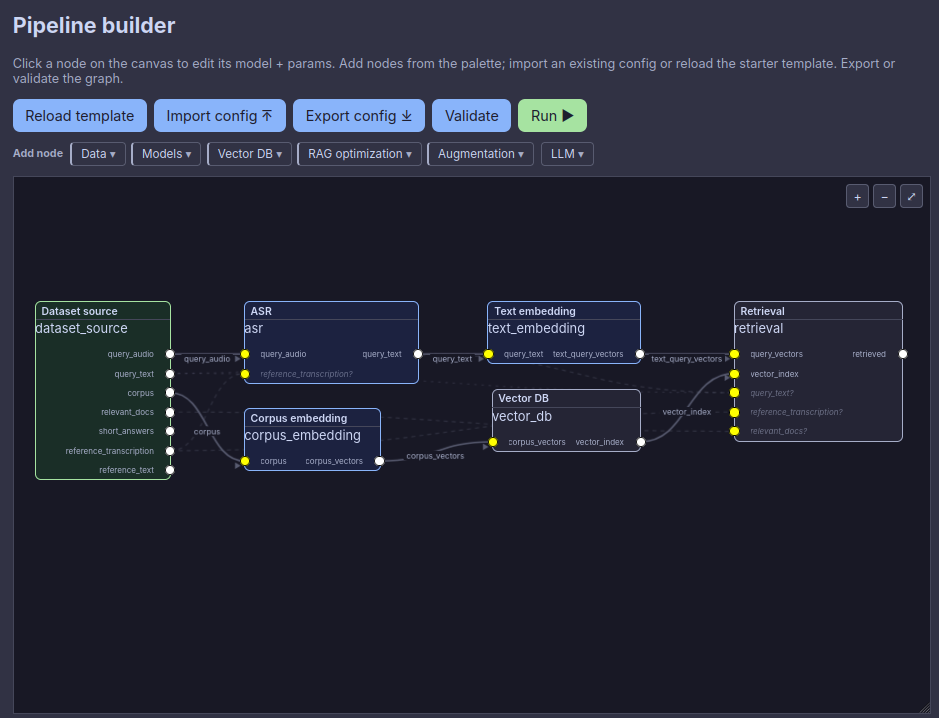
\includegraphics[width=0.92\linewidth]{figures/builder_ui.png}
    \caption{Edytor wizualny grafu. Gniazda węzłów opisane są nazwami artefaktów, a wejścia
    opcjonalne zaznaczono kursywą. Pokazany graf odpowiada ścieżce kaskadowej.}
    \label{fig:builderUi}
\end{figure}

\subsection{Ograniczenia i kod źródłowy}
\label{sec:ograniczenia}
Przyjęte założenia wyznaczają trzy granice zastosowania. Graf jest ustalony w chwili budowy, więc
sterowanie zależne od danych trzeba zamknąć w jednym węźle, którego wnętrze pozostaje
nieprzejrzyste dla proweniencji. Przebieg wykonywany jest w obrębie jednej maszyny, a większy
korpus obsługuje przetwarzanie oknami, nie rozdzielenie pracy między osobne węzły obliczeniowe.
Granicą pozostaje zatem pojemność jednej maszyny. Generacja odpowiedzi i sędzia korzystają z zewnętrznej
usługi modelu językowego, więc ich odtwarzalność jest względna wobec serwera, a jakość odpowiedzi
ocenia sędzia automatyczny wraz z heurystykami leksykalnymi, nie klinicysta.

Osobne ograniczenia wnosi sam zbiór badawczy. Ścieżka głosowa nie pochodzi z nagrań, lecz jest
syntezowana w czasie wykonania, więc nie obejmuje zmienności osobniczej mówcy, wad wymowy ani
zakłóceń otoczenia. Według wiedzy autorów nie istnieje też publiczny medyczny zbiór pytań i dokumentów w języku polskim
o strukturze wymaganej do oceny wyszukiwania, dlatego PubMedQA przetłumaczono na polski modelem
językowym. Tłumaczenie maszynowe wnosi własny błąd, uproszczenia terminologii i kalki składniowe,
który nakłada się na mierzone różnice między architekturami i którego niniejsza praca od nich nie
rozdziela. Zbiór polski jest przy tym mały, sto pytań i sto dokumentów; konsekwencje tej skali
dla zasięgu wniosków omówiono w podrozdziale~\ref{sec:jezyk}.

Implementację w języku Python udostępniono na licencji MIT wraz z konfiguracjami opisanych
eksperymentów \cite{reteva}.

\section{Eksperymenty i wyniki}
\label{sec:eksperymenty}
Podrozdział przedstawia pomiary wykonane za pomocą opisanego wyżej systemu. Porównywane warianty są
konfiguracjami tego samego grafu, przedstawionego w podrozdziale \ref{sec:sciezka}. Przedmiotem
porównania są dwie architektury przetwarzania zapytania głosowego: klasyczna kaskada, w której
nagranie jest najpierw transkrybowane, a dopiero powstały tekst embeddowany w przestrzeni
wektorowej, oraz proponowane rozwiązanie, w którym reprezentacja latentna modelu ASR jest
dopasowywana wprost do przestrzeni modelu embeddingowego. Obu towarzyszy trzecia konfiguracja,
pozbawiona ścieżki głosowej i pełniąca rolę punktu odniesienia, a nie rozwiązania poddanego ocenie.
Pomiary prowadzone są na dwóch zestawach danych opisanych w podrozdziale~\ref{sec:zbiory}.
Porównywane konfiguracje przetwarzają w obrębie jednego zestawu ten sam zbiór pytań, więc różnice
liczone są parami.

\subsection{Metodologia}

\subsubsection{Zbiory danych}
\label{sec:zbiory}
Podstawą porównania jest zbiór PubMedQA \cite{jin2019pubmedqa}, w którym każde pytanie ma przypisany
artykuł źródłowy, pełniący rolę jedynego dokumentu istotnego. Zbiór występuje w dwóch
konfiguracjach: anotowanej przez ekspertów, liczącej tysiąc pytań, oraz etykietowanej automatycznie,
obejmującej ponad dwieście tysięcy pytań. Wybrano konfigurację anotowaną, mimo że jest o dwa rzędy
wielkości mniejsza, ponieważ w konfiguracji automatycznej ponad dziewięćdziesiąt procent odpowiedzi
to ,,tak'', a klasa ,,może'' praktycznie nie występuje. Trafność decyzji mierzona na takim materiale
nie odróżniałaby systemu od odpowiadania stałą wartością.

Eksperymenty prowadzi się na dwóch zestawach, z których każdy odpowiada na inne pytanie. Zestaw
główny to całość konfiguracji anotowanej: tysiąc pytań i tysiąc dokumentów, w całości
anglojęzycznych. Służy on porównaniu samych architektur przetwarzania, ponieważ daje moc testu oraz
dziesięciokrotnie większy korpus, w którym trafienie w dokument istotny jest odpowiednio
trudniejsze. Zestaw językowy liczy sto pytań, jest ścisłym podzbiorem poprzedniego i występuje w
trzech wariantach językowych; służy zmierzeniu kosztu zadania pytania po polsku oraz ocenie
odpowiedzi generowanych z pełnych artykułów.

Podział ten wynika z natury badanego zjawiska. Różnica między kaskadą a dopasowaniem reprezentacji
latentnych bierze się z tego, że pierwsza przepuszcza sygnał przez pośrednią postać dyskretną, a
druga nie; mechanizm ten nie zależy od języka zapytania. Rozstrzygnięcie, która architektura jest
lepsza, wymaga zatem przede wszystkim mocy statystycznej, którą daje zestaw większy. Osobnym
pytaniem jest to, ile jakości ubywa, gdy zapytanie pada po polsku, i na nie odpowiada zestaw
mniejszy.

Zestaw językowy liczy sto pytań, a nie tysiąc, z dwóch powodów naraz. Po pierwsze wariant z korpusem
polskim wymaga przetłumaczenia każdego dokumentu, a tłumaczenie tysiąca abstraktów przekraczało
dostępne zasoby. Po drugie ocena generacji wymaga pełnych tekstów artykułów, te zaś są dostępne
wyłącznie dla podzbioru: spośród tysiąca artykułów konfiguracji anotowanej pełny tekst udaje się
pobrać z otwartego repozytorium PMC dla stu piętnastu, czyli dla 11,5 procent. Wybrano sto pytań
spełniających oba warunki naraz, dzięki czemu ten sam zestaw obsługuje część językową i część
generacyjną.

Korpus zestawu językowego przygotowano w trzech wariantach, aby rozdzielić dwa efekty, które w
pojedynczym pomiarze pozostawałyby ze sobą splecione. Wariant pierwszy zestawia pytania polskie z
korpusem angielskim i odpowiada sytuacji realnej, ponieważ literatura biomedyczna jest w
przeważającej mierze anglojęzyczna. Wariant drugi zestawia pytania polskie z korpusem
przetłumaczonym i pozwala zmierzyć, ile jakości traci samo przejście między językami. Wariant
trzeci, w całości anglojęzyczny, pokazuje koszt użycia języka polskiego niezależnie od modalności.
Podział ten odpowiada wprost ograniczeniom omówionym w podrozdziale \ref{sec:motywacja}. Wszystkie
trzy warianty obejmują te same sto pytań i te same sto dokumentów, rozpoznawane po wspólnych
identyfikatorach, więc różnice liczone są parami, pytanie po pytaniu.

Tłumaczenie na język polski wykonano modelem językowym, osobno dla treści pytania, tytułu dokumentu,
abstraktu i odpowiedzi referencyjnej; etykiety decyzji pozostawiono w postaci oryginalnej, ponieważ
ocena porównuje je z literałami zbioru. Pełne teksty artykułów pozostają wyłącznie anglojęzyczne,
zatem ocena odpowiedzi generowanych z pobranego kontekstu przebiega zawsze na materiale angielskim,
także wtedy, gdy pytanie zadano po polsku. Charakterystykę obu zbiorów zestawiono w
tabeli~\ref{tab:zbior}.

\begin{table}[h]
\centering
\small
\begin{tabular}{@{}L{6.4cm}L{2.5cm}L{2.5cm}L{2.5cm}@{}}
\toprule
& \textbf{Zestaw główny} & \multicolumn{2}{c}{\textbf{Zestaw językowy}} \\
\cmidrule(lr){2-2}\cmidrule(lr){3-4}
\textbf{Wielkość} & angielski & angielski & polski \\
\midrule
Liczba pytań                              & 1000          & 100        & 100 \\
Liczba dokumentów w korpusie              & 1000          & 100        & 100 \\
Dokumenty istotne na pytanie              & 1             & 1          & 1 \\
Rozkład odpowiedzi (tak / nie / może)     & 552/338/110   & 56/36/8    & 56/36/8 \\
Długość pytania (mediana, słowa)          & 13            & 12,5       & 13 \\
Długość abstraktu (mediana, słowa)        & 201           & 209        & 206 \\
Długość pełnego artykułu (mediana, słowa) & ---           & 3286       & --- \\
\bottomrule
\end{tabular}
\caption{Charakterystyka zbiorów użytych w eksperymentach. Zestaw językowy jest ścisłym podzbiorem
głównego, a jego wersje językowe obejmują te same pytania i dokumenty, rozpoznawane po wspólnych
identyfikatorach. Pełne teksty artykułów są dostępne wyłącznie w wersji angielskiej zestawu
językowego.}
\label{tab:zbior}
\end{table}

Oba korpusy są małe wobec zastosowania rzeczywistego, w którym system przeszukuje zbiór o kilka
rzędów wielkości większy, więc bezwzględne wartości metryk rankingowych należy czytać jako
optymistyczne. Dotyczy to zwłaszcza korpusu stu dokumentów, gdzie nawet losowy ranking trafia w
dokument istotny co dziesiąte pytanie przy progu odcięcia równym dziesięć. Nie unieważnia to
porównania, ponieważ wszystkie konfiguracje pracują na tym samym korpusie, a przedmiotem oceny jest
różnica między nimi, nie poziom bezwzględny. Ponieważ zestaw językowy jest podzbiorem głównego,
wynik konfiguracji anglojęzycznej można policzyć na obu i sprawdzić, czy setka zachowuje się jak
tysiąc; rozbieżność wskazywałaby, że efekt przypisany językowi bierze się z doboru podzbioru.

Ścieżka audio nie pochodzi z nagrań, lecz jest syntezowana w czasie wykonania przez węzeł syntezy
mowy. Wybór ten zapewnia, że wszystkie porównywane konfiguracje pracują na identycznym sygnale
wejściowym, więc różnice w wynikach nie mogą pochodzić z różnic między nagraniami. Ceną jest
ograniczona zmienność mowy: sygnał syntetyczny nie obejmuje pełnego zakresu cech osobniczych mówcy,
wad wymowy ani zakłóceń otoczenia. Wnioski o odporności należy zatem odnosić do zmienności
wprowadzonej celowo, opisanej w podrozdziale \ref{sec:odpornosc}, a nie do zmienności naturalnej.

\subsubsection{Porównywane architektury}
Porównaniu podlegają trzy konfiguracje. Pierwsza pomija ścieżkę głosową i kieruje do wyszukiwania
tekst pytania. Nie jest ona rozwiązaniem poddanym ocenie, lecz wyznacza górną granicę jakości
osiągalnej przy danym korpusie i danym modelu embeddingowym. Bez tego odniesienia nie sposób
rozstrzygnąć, czy różnica między pozostałymi konfiguracjami wynika z architektury, czy z trudności
samego zadania wyszukiwania. Druga konfiguracja to kaskada, w której nagranie przechodzi przez model
ASR, a powstała transkrypcja przez model embeddingowy. Trzecia to dopasowanie reprezentacji
latentnych, w którym wyjście enkodera ASR rzutowane jest wprost do przestrzeni modelu embeddingowego
przez adapter wytrenowany w rozdziale \ref{sec:latentTranslation}.

\todo{Uzupełnić listę wykorzystanych modeli ASR i embeddingowych wraz z uzasadnieniem doboru, opartym na wnioskach z rozdziałów \ref{sec:latent} i \ref{sec:latentTranslation}}

\subsubsection{Metryki}
Jakość wyszukiwania oceniana jest metrykami rankingowymi zdefiniowanymi w podrozdziale
\ref{sec:metryki}. Dobór metryk ogranicza jednak struktura zbioru: każde pytanie ma dokładnie
jeden dokument istotny, czyli artykuł, z którego powstało. Dla pojedynczego pytania skuteczność
wyszukiwania przyjmuje wtedy wartość zero albo jeden, precyzja na progu $k$ jest jej stałą
wielokrotnością, a średnia precyzja pokrywa się z odwrotnością rangi. Raportuje się zatem Recall@k
oraz NDCG@k dla progów $k \in \{1,5,10\}$, a także MRR liczoną dla całej listy wyników; Precision@k
i MAP pominięto, ponieważ na tych danych nie wnoszą nic ponad to, co zawierają pozostałe miary.
Metryki liczone są osobno dla każdego pytania, co jest warunkiem zastosowania testu sparowanego oraz
analizy przedstawionej w podrozdziale \ref{sec:prog}.

Jakość transkrypcji mierzona jest wskaźnikiem błędu na poziomie słów i znaków. Wielkości te dotyczą
wyłącznie konfiguracji kaskadowej, ponieważ pozostałe dwie transkrypcji nie wytwarzają. Nie są więc
przedmiotem porównania między architekturami, lecz zmienną objaśniającą w analizie zależności między
jakością transkrypcji a jakością wyszukiwania.

\subsubsection{Aparat statystyczny}
Każdą wielkość zbiorczą podaje się wraz z przedziałem ufności wyznaczonym metodą losowania ze
zwracaniem (ang.\ \textit{bootstrap}), a różnice między konfiguracjami ocenia się testem sparowanym,
ponieważ wszystkie konfiguracje przetwarzają ten sam zbiór pytań. Zmienność między pytaniami jest
znacznie większa niż różnice między architekturami, więc test dla prób niezależnych miałby na tych
danych zbyt małą moc, by wykryć badane różnice.

Porównanie architektur, analizę odporności, wyznaczenie progu jakości transkrypcji oraz pomiary
zasobów prowadzi się na zestawie tysiąca pytań, ponieważ wszystkie wymagają mocy testu. Efekt języka
oraz ocenę odpowiedzi generowanych z kontekstu prowadzi się na zestawie stu pytań, ponieważ tylko on
istnieje w wariantach językowych i tylko dla niego dostępne są pełne teksty. Każde porównanie opiera
się na pełnym komplecie par danego zestawu; sto par jest liczbą skromną, lecz przekracza próg,
poniżej którego framework oznacza wynik jako obarczony małą mocą.

\subsection{Porównanie architektur w warunkach czystych}
\label{sec:czyste}
Podrozdział przedstawia wyniki wyszukiwania dla nagrań niezakłóconych na zestawie tysiąca pytań.
Jest to zasadnicze porównanie niniejszej pracy: kaskada zestawiona z dopasowaniem reprezentacji
latentnych, obie odniesione do górnej granicy wyznaczonej przez konfigurację tekstową. Odniesienie
do tej granicy rozdziela dwa źródła utraty jakości, przejście na modalność mowy oraz wybór
architektury przetwarzania, których łączny efekt w pojedynczym pomiarze pozostawałby
nierozróżnialny.

\todo{Uzupełnić tabelę wyników oraz ich omówienie po wykonaniu przebiegów}

\subsection{Koszt zadania pytania po polsku}
\label{sec:jezyk}
Podrozdział powtarza porównanie architektur na zestawie stu pytań, w trzech wariantach językowych
opisanych w podrozdziale~\ref{sec:zbiory}, i na tej podstawie rozdziela utratę jakości wnoszoną
przez sam język od utraty wnoszonej przez modalność. Wariant w całości anglojęzyczny odtwarza
warunki podrozdziału~\ref{sec:czyste} na mniejszej próbie, więc pełni podwójną rolę: wyznacza punkt
odniesienia dla dwóch pozostałych wariantów, a zarazem pozwala sprawdzić, czy setka zachowuje się
jak tysiąc, z którego została wybrana.

Rozstrzygnięcia wymaga zwłaszcza różnica między wariantem jednojęzykowym polskim a międzyjęzykowym,
ponieważ wskazuje ona, jaka część utraty jakości bierze się z przekraczania granicy języka przez
samo zapytanie, a jaka z tego, że polszczyzna jest dla użytych modeli językiem gorzej
reprezentowanym niż angielski.

\todo{Uzupełnić zestawienie wyników dla trzech wariantów językowych oraz omówienie po wykonaniu przebiegów}

\subsection{Jakość odpowiedzi generowanych z pobranego kontekstu}
\label{sec:generacja}
Wyszukiwanie jest w zastosowaniu klinicznym środkiem, a nie celem: użytkownik oczekuje odpowiedzi,
nie listy dokumentów. Podrozdział sprawdza zatem, czy przewaga jednej architektury nad drugą,
zmierzona metrykami rankingowymi, przenosi się na jakość odpowiedzi generowanej z pobranego
kontekstu. Przejście to nie jest oczywiste, ponieważ model językowy potrafi odpowiedzieć poprawnie
mimo niedoskonałego rankingu, o ile potrzebny fragment znalazł się w kontekście, i odwrotnie ---
potrafi zawieść przy rankingu poprawnym.

Kontekstem są pełne artykuły, a nie abstrakty, ponieważ abstrakt rzadko zawiera dane liczbowe
potrzebne do uzasadnienia odpowiedzi. Jest to jednak kontekst wyłącznie angielski, więc konfiguracje
z pytaniem polskim pracują w układzie międzyjęzykowym również na etapie generacji. Mediana długości
artykułu przekracza trzy tysiące słów, czyli około siedemnastokrotność abstraktu, co przy kilku
pobranych dokumentach wyczerpuje typowe okno kontekstowe modelu językowego. Liczbę dokumentów
podawanych modelowi dobrano więc z uwzględnieniem tego ograniczenia.

Ocena obejmuje metryki opisane w podrozdziale \ref{sec:rag}: trafność decyzji wobec etykiety zbioru,
podobieństwo ROUGE do odpowiedzi referencyjnej, wskaźnik halucynacji, pokrycie kontekstu oraz oceny
sędziego automatycznego. Pokrycie kontekstu pełni tu rolę rozstrzygającą, ponieważ oddziela
niepowodzenie wyszukiwania od niepowodzenia generacji: jego niska wartość oznacza, że potrzebnej
treści w pobranych dokumentach nie było, więc winą za błędną odpowiedź nie można obciążać modelu
językowego.

\todo{Uzupełnić zestawienie metryk odpowiedzi oraz omówienie po wykonaniu przebiegów}

\subsection{Odporność na degradację sygnału}
\label{sec:odpornosc}
Podrozdział przedstawia jakość wyszukiwania jako funkcję stosunku sygnału do szumu, osobną krzywą
dla każdej z porównywanych architektur, a ponadto wpływ zmiany tempa mowy. Celem
jest sprawdzenie hipotezy o odmiennym charakterze degradacji obu rozwiązań. W kaskadzie błąd
transkrypcji usuwa termin z zapytania bezpowrotnie, ponieważ dalsze etapy nie mają już dostępu do
sygnału, z którego termin powstał. W dopasowaniu reprezentacji latentnych sygnał nie przechodzi
przez pośrednią postać dyskretną, więc oczekuje się degradacji łagodniejszej, rozłożonej na
wszystkie wymiary reprezentacji zamiast skupionej w pojedynczym utraconym słowie.

\todo{Uzupełnić wykresy jakości w funkcji stosunku sygnału do szumu oraz omówienie po wykonaniu przebiegów}

\subsection{Zależność jakości wyszukiwania od jakości transkrypcji}
\label{sec:prog}
Podrozdział zestawia jakość wyszukiwania z jakością transkrypcji, pytanie po pytaniu, i na tej
podstawie wyznacza próg jakości transkrypcji, poniżej którego kaskada przestaje przewyższać
rozwiązanie proponowane. Ponieważ konfiguracja latentna transkrypcji nie wytwarza, jej wyniki
przypisuje się wartości wskaźnika błędu osiągniętej przez kaskadę na tym samym pytaniu. Zestawienie
takie jest możliwe wyłącznie dzięki temu, że obie konfiguracje przetwarzają ten sam zbiór, a ich
wyniki pozostają powiązane identyfikatorem pytania.

Jest to wynik, który najbardziej bezpośrednio przekłada się na regułę doboru architektury. Znając
spodziewaną jakość transkrypcji w danym zastosowaniu, można z niego odczytać, która ścieżka
przetwarzania jest korzystniejsza, bez powtarzania całego porównania.

\todo{Uzupełnić wykres zależności oraz wyznaczoną wartość progu wraz z przedziałem ufności}

\subsection{Wykorzystanie zasobów i prędkość wyszukiwania}
\label{sec:zasoby}
Podrozdział przedstawia opóźnienie pełnej ścieżki przetwarzania, szczytowe zużycie pamięci karty
graficznej, przepustowość oraz rozmiar indeksu. Oczekiwana przewaga konfiguracji latentnej wynika z
pominięcia dekodowania autoregresyjnego: kaskada musi wytworzyć transkrypcję element po elemencie,
podczas gdy ścieżka latentna wykonuje pojedyncze przejście w przód przez enkoder oraz adapter.
Pomiary te są dla wyboru architektury równorzędne z jakością, ponieważ w zastosowaniu klinicznym o
przydatności systemu decyduje nie tylko trafność wyników, lecz także czas oczekiwania na nie.

\todo{Uzupełnić zestawienie pomiarów zasobów i opóźnień po wykonaniu przebiegów}

\subsection{Wnioski}
Podrozdział zestawia obie architektury wraz z ich osiągami, wskazując warunki, w których przewaga
jednej z nich jest rozstrzygająca, oraz warunki, w których wybór pozostaje kompromisem między
jakością a kosztem obliczeniowym.

\todo{Uzupełnić wnioski po zebraniu wyników z podrozdziałów \ref{sec:czyste}--\ref{sec:zasoby}}


% --- Podsumowanie ---
\chapter{Podsumowanie\aut{T.P.}}
\label{sec:podsumowanie}
%LTex: language=pl
W ramach tej pracy przeprowadzono szereg powiązanych ze sobą eksperymentów, pozwalających na analizę właściwości modeli ASR w ramach wykorzystania ich jako część potoku przetwarzania w systemach wyszukiwania informacji za pomocą sygnału mowy. Rozdział 3 koncentrował się na właściwościach przestrzeni latentnych obecnych w enkoderach dostępnych modeli automatycznego rozpoznawania mowy w świetle enkodowania semantyki danych wejściowych, jak i możliwości zastosowania dodatkowego przetwarzania danych enkodowanych przez te modele. Wnioski pozyskane z tych eksperymentów posłużyły w doborze odpowiednich enkoderów audio w ramach treningu proponowanych w tej pracy modeli, \textit{Attention Pool Model} i \textit{Embedding Alignment Model}, które wytrenowane zostały na zbiorze AdmedVOICE w celu semantycznego wyszukiwania dokumentów tekstowych za pomocą sygnału mowy. Rozdział 5 zawierał testy modeli w ramach różnych scenariuszy testowych, oferując porównanie różnych podejść, wykorzystujących zarówno proponowane architektury, jak i klasyczne podejście kaskadowe oparte na transkrypcji sygnału mowy.

\section{Pytania badawcze}
\subsection{Czy reprezentacje ukryte generowane przez modele ASR zawierają wystarczającą informację semantyczną do realizacji zadań wyszukiwania informacji?}
W wyżej wymienionej formie, eksperymenty w tej pracy wykazały częściową zdolność wykorzystania modeli ASR w celu wyszukiwania informacji podobnych semantycznie w ramach domeny ogólnej. Wyniki badań w Rozdziale 3, wskazują na dosyć silną zdolność dyskryminacji między nagraniami mowy podobnymi semantycznie, a różnymi, w szczególności dla modeli SeamlessM4T i Whisper. Pośrednim potwierdzeniem tego wniosku jest stabilność treningu modeli \textit{Attention Pool Model} i \textit{Embedding Alignment Model}, wykorzystujących enkodery wyżej wymienionych modeli ASR, choć nie oznacza to bezpośrednio nacechowania semantycznego danych przetworzonych przez takie enkodery (Rozdział 4). Jednakże, na jednoznaczne potwierdzenie tej tezy nie pozwalają wyniki uzyskane w ramach eksperymentów zawartych w Rozdziale 5, gdzie proponowane w tej pracy architektury nie były w stanie dorównać wyszukiwaniu kaskadowemu lub modelowi embeddingowemu SONAR. Nie może oznaczać to jednak braku przydatności architektur \textit{APM} i \textit{EAM} w ramach wyszukiwania, ponieważ najprawdopodobniej najważniejszym czynnikiem prowadzącym do wyraźnie gorszych rezultatów wyszukiwania dla tych modeli jest ilość danych wykorzystanych w ramach treningu, będąca w niektórych przypadkach $10000$ razy mniejsza niż dla gotowych modeli ewaluowanych w ramach porównania \cite{m4t}. Podsumowując, nie udało się jednoznacznie udowodnić zdatności proponowanych architektur modeli wykorzystujących enkodery modeli ASR w ramach wyszukiwania informacji, lecz w pracy wykazano wiele przesłanek pozwalających sądzić, że przy większej ilości danych treningowych, architektury te mogłyby dobrze radzić sobie w ramach tego zadania.
\subsection{Czy modele embeddingowe oparte na enkoderach modeli ASR są w stanie dokładnie enkodować semantykę danych wejściowych?}
Powiązana z poprzednim pytaniem, hipoteza ta została potwierdzona w ramach eksperymentów opisanych w Rozdziale 4. Obie proponowane w tej pracy architektury wykazały się stabilnością i wysokimi wynikami maksymalizowanych metryk w ramach treningu. Pomijając wymaganie obecności modelu w ramach całościowego systemu wyszukiwania informacji i rozpatrując zarówno \textit{Attention Pool Model} i \textit{Embedding Alignment Model} w izolacji, stanowią one obiecujące metody tworzenia multimodalnych modeli embeddingowych. Architektura \textit{APM}, celem której treningu jest maksymalizacja podobieństwa między wektorami generowanymi przez gałąź przetwarzania sygnału audio i analogicznymi wektorami dla transkrypcji tych nagrań generowanymi przez pretrenowany model embeddingowy skutecznie dokonuje transformacji między dwoma przestrzeniami embeddingowymi, oferując szybsze działanie modelu niż w przypadku podejścia kaskadowego (Rozdział 5). Model \textit{EAM} przypomina za to bardziej pełnoprawny model embeddingowy, trening którego wymaga potencjalnie ogromnej ilości danych, lecz pozwala na wykorzystanie istniejących modeli pełniących funkcję enkoderów w ramach całościowego systemu. Dodatkową zaletą jest potencjał wykorzystania treningu wstępnego nienadzorowanego, potencjalnie pozwalając na ograniczenie wielkości wymaganych danych zawierających etykiety (pary nagranie mowy -- transkrypcja), które w ramach tej pracy nie poprawiło jakości modelu i trening metodą Data2Vec był niestabilny -- nie świadczy to jednak jednoznacznie o braku przydatności tej metody, lecz w celu wykorzystania tego procesu, należałoby powtórzyć eksperyment z większą ilością danych (Rozdział 4).
\subsection{Jak jakość wyszukiwania opartego na reprezentacjach ukrytych wypada w porównaniu z podejściem kaskadowym (ASR $\rightarrow$ embedding tekstowy)?}
Jakość wyszukiwania jest pojęciem zależnym od oczekiwań użytkownika docelowego całościowego systemu. W Rozdziale 5 przedstawiono szereg porównań i metryk, pozwalających na kompleksowe podejście do wyboru rozwiązania w zależności od wymagań użytkowników systemu. Zaproponowane w tej pracy modele \textit{Attention Pool Model} i \textit{Embedding Alignment Model} cechują się większą prędkością przetwarzania niż klasyczne podejście kaskadowe oparte na transkrypcji, którego ogromną zaletą jest większa wyjaśnialność poprzez produkcję transkrypcji zapytania audio, co potwierdza hipotezę zaproponowaną we wprowadzeniu pracy. W ramach metryk oceniających dokładność wyszukiwania informacji, \textit{APM} i \textit{EAM} wypadają o wiele gorzej niż ewaluowane kaskadowe potoki przetwarzania. Model SONAR, będący multimodalnym modelem embeddingowym, radził sobie lepiej niż proponowane w tej pracy architektury, jednakże nadal nie był w stanie prześcignąć podejścia kaskadowego wykorzystującego model embeddingowy Jina, nawet dla wysokich wartości błędu WER dla transkrypcji (Rozdział 5, Rysunek \ref{fig:wynikiWer}). Zjawisko to pokazuje, że dobór odpowiedniego modelu odpowiedzialnego za semantyczne osadzenie tekstu jest o wiele ważniejsze niż minimalizacja WER w wykorzystanym modelu ASR generującego transkrypcje zapytań w ramach podejścia kaskadowego.
\subsection{Jaki wpływ na jakość obu podejść ma język zapytania (polski a angielski)?}
Poszukiwania odpowiedzi na to pytanie zostały opisane głównie w Rozdziale 5, jak i częściowo w Rozdziale 3. W ramach eksperymentów ewaluujących zachowanie przestrzeni latentnej modeli ASR, zbadane zostało zjawisko powstania osobnych grup reprezentujących różne języki, w ramach którego pokazano pewną inwariancję enkodowanych reprezentacji w świetle języka przetwarzanej wypowiedzi (z wyjątkiem modelu Whisper, gdzie zaobserwowano wyraźną separację między językiem polskim i angielskim). Obserwacja ta została potwierdzona w ramach eksperymentu wielojęzykowego wyszukiwania informacji dla benchamarku PubmedQA w Rozdziale 5 (Rysunek \ref{fig:wynikiJezykAudio}), gdzie model \textit{APM} uczony na danych w języku polskim, wyraźnie gorzej poradził sobie w ramach wyszukiwania informacji dla zapytania w języku angielskim. Z kolei model \textit{EAM} osiągnął lepsze wyniki dla zapytania w języku angielskim mimo nauki na danych w języku polskim. Wyraźne różnice obecne w ramach modeli wykorzystujących translację przestrzeni latentnych nie zostały zaobserwowane przy podejściu kaskadowym, dla którego jakość wyszukiwania utrzymywała się na podobnie wysokim poziomie (zarówno błąd transkrypcji WER, jak i jakość wyszukiwania samego modelu embeddingowego). Podejście kaskadowe cechuje się lepszymi metrykami i stabilnością dla zadania wyszukiwania wielojęzykowego niż podejście latentne.

\section{Dyskusja}
Podczas formułowania zakresu tej pracy wyłoniły się dwa główne nurty, które zostały w niej poruszone. Pierwszym z nich jest sama ewaluacja różnych podejść wyszukiwania informacji za pomocą zapytania głosowego, opisana w Rozdziale 5. Proponowany system pozwala na kompleksowe badania nad różnymi rozwiązaniami wykorzystującymi dodatkowe metody przetwarzania artefaktów generowanych w ramach łańcucha przetwarzania (m.in. augementacja danych, postprocessing embeddingów, korekcja transkrypcji) na różnych zbiorach danych. Nie jest to narzędzie przydatne w ramach eksperymentów przeprowadzonych w ramach tej pracy, lecz może również stanowić pomoc w dalszych badaniach nad zadaniem wyszukiwania informacji za pomocą zapytania głosowego, nie tylko w bazach specjalistycznych. Wracając do samych eksperymentów, ważnym usprawnieniem byłoby stworzenie dedykowanego zbioru danych w języku polskim zawierającym zapytanie audio, jego transkrypcję i listę rankingową najbardziej powiązanych dokumentów. Aktualne badania oparte na tłumaczeniu maszynowym streszczeń artykułów ze zbioru PubmedQA i zbiorze AdmedVoice stanowią niewątpliwie cenne zbiory pozwalające na częściową ewaluację wyszukiwania, lecz posiadanie wyłącznie jednego dokumentu oznaczonego jako mający znaczenie dla zapytania (ang. \textit{relevant}) stanowi duże ograniczenie w kompleksowej ewaluacji całościowego systemu, potencjalnie zaburzając otrzymane wyniki. Dodatkowo, przez koszty związane z procesem tłumaczenia angielskich tekstów na język polski, jedynie 10\% wszystkich artykułów zostało przetłumaczone, zmniejszając rozmiar zbioru danych, na którym oparta była ewaluacja. Uwzględnienie pełnego zbioru przetłumaczonego na język polski może stanowić duże usprawnienie w świetle dokładności metryk opisujących wyniki wyszukiwania. Niezbędnym elementem wymagającym dalszej ewaluacji jest wpływ modelu embeddingowego na jakość wyszukiwania metodą kaskadową. W tej pracy przetestowano 3 różne modele, w ramach których JinaV4 osiągała najlepsze wyniki dla różnych metod ewaluacji. Wartościowym uzupełnieniem tych badań byłaby dodatkowa ewaluacja kolejnych modeli embeddingowych, w szczególności tych dedykowanych do działania w ramach domeny medycznej. \\

Kolejnym aspektem tej pracy były proponowane architektury modeli wykorzystujących translację przestrzeni latentnych enkoderów modeli ASR, \textit{Attention Pool Model} i \textit{Embedding Alignment Model}. W ramach treningu na zbiorze danych AdmedVoice, obie z proponowanych architektur cechowały się stabilnym treningiem i wysokimi wartościami metryk maksymalizowanych w ramach tego procesu na zbiorze testowym. Zgodnie z hipotezą przedstawioną we wprowadzeniu, czas potrzebny do przetworzenia zapytania w formie nagrania mowy i wygenerowania wektora będącego jego reprezentacją był mniejszy niż w podejściu kaskadowym, co stanowi niewątpliwą przewagę tych architektur nad podejściem kaskadowym. Jednakże, w ramach ich całościowej ewaluacji jako część systemu wyszukiwania informacji, nie były one w stanie dorównać przetwarzaniu opartym na generowaniu transkrypcji. Reiterując wnioski powstałe w ramach odpowiedzi na pytania badawcze, najprawdopodobniej winna jest temu zjawisku ilość danych wykorzystanych w ramach ich treningu. Model SONAR, będący multimodalnym modelem embeddingowym, wykazał się większą skutecznością w ramach wyszukiwania informacji, mimo braku dostosowania go do operowania w ramach domeny medycznej. Oznacza to przewagę zdolności generalizacji modelu, uzyskanej na podstawie większej ilości danych treningowych, nad dedykowanym modelem przystosowanym wyłącznie do przetwarzania danych w ramach mowy i tekstów klinicznych. W celu rzetelnego porównania architektur, należałoby wytrenować modele \textit{APM} i \textit{EAM} na o wiele większych zbiorach danych, zawierających również dane spoza domeny medycznej, w celu zwiększenia ich zdolności generalizacyjnej. Praca ta wykazała, że architektury te produkują modele stabilne i zdolne do wyszukiwania informacji, jednakże z tak małą ilością danych obecnych w zbiorze treningowym, nie są one w stanie prześcignąć innych poddanych ewaluacji modeli. Dodatkowo, uczenie modelu \textit{Embedding Alignment Model} z wykorzystaniem treningu wstępnego wymaga dalszej pracy, również na o wiele większym zbiorze danych, w celu zbadania potencjalnych zysków z zastosowania takiego podejścia.


% --- Bibliografia ---
\printbibliography

% --- Appendix ---
\appendix
% w spisie treści: "Dodatek A." zamiast samego "A."
\titlecontents{chapter}[0em]{}{Dodatek \thecontentslabel.\quad}{}{\dotfill\contentspage}
% podpisy rysunków w dodatkach: "Dodatek A.1." zamiast "Rys. A.1."
\renewcommand{\figurename}{Dodatek}
\titleformat{\chapter}[hang]{\bfseries\fontsize{12pt}{24pt}\selectfont\hyphenpenalty=10000\exhyphenpenalty=10000}{Dodatek \thechapter.\quad}{0pt}{\MakeUppercase{#1}}
\section*{Semantyczne reprezentacje wektorów cech modeli ASR}
\FloatBarrier
\subsection*{Analiza enkodowania znaczenia semantycznego mowy}

\begin{figure}[!htbp]
    \centering
    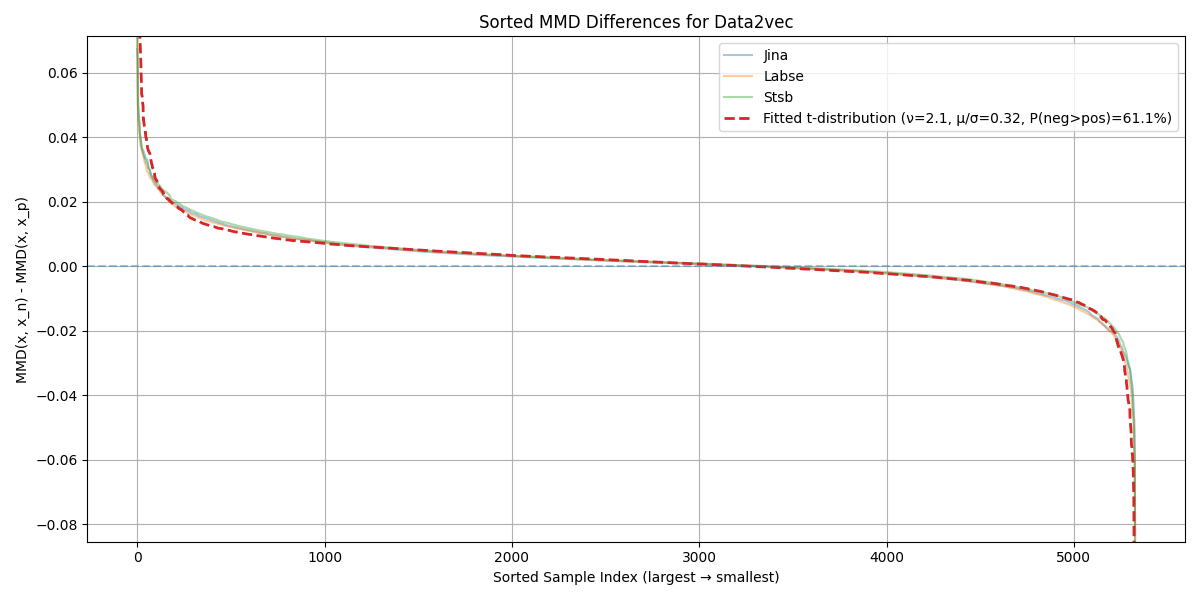
\includegraphics[width=0.8\linewidth]{figures/semantics/data2vec.png}
    \caption{Rozkład wartości różnicy podobieństw dla Data2Vec w ramach zbioru \textit{Medical Speech, Transcription, and Intent}}
    \label{fig:latent:medicalData2Vec}
\end{figure}

\begin{figure}[!htbp]
    \centering
    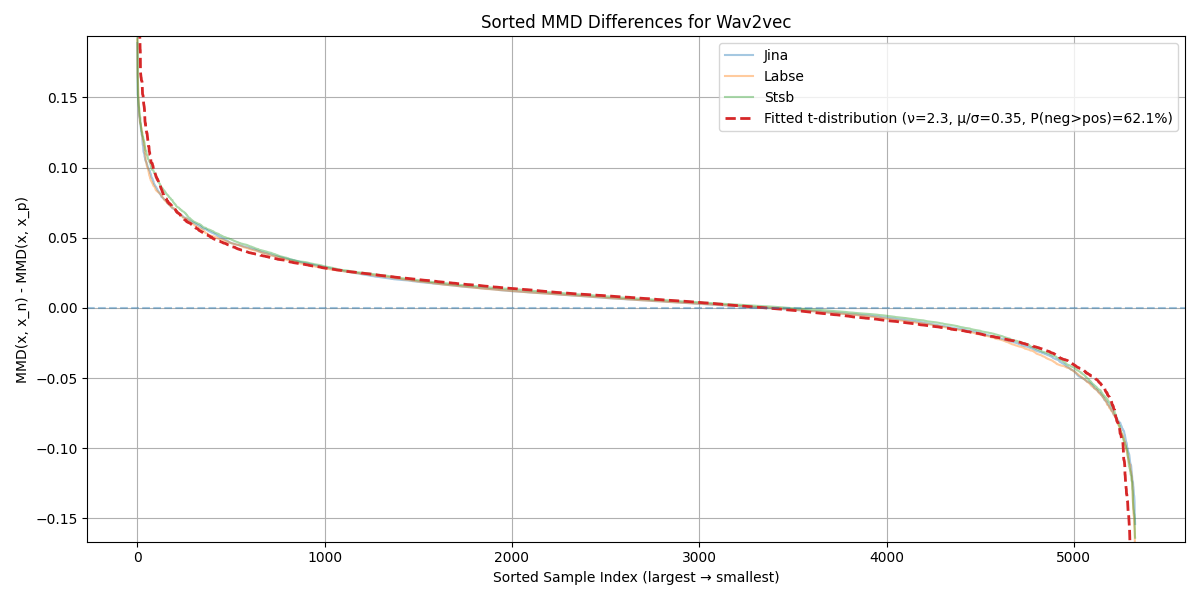
\includegraphics[width=0.8\linewidth]{figures/semantics/wav2vec.png}
    \caption{Rozkład wartości różnicy podobieństw dla Wav2Vec w ramach zbioru \textit{Medical Speech, Transcription, and Intent}}
    \label{fig:latent:medicalWav2Vec}
\end{figure}

\begin{figure}
    \centering
    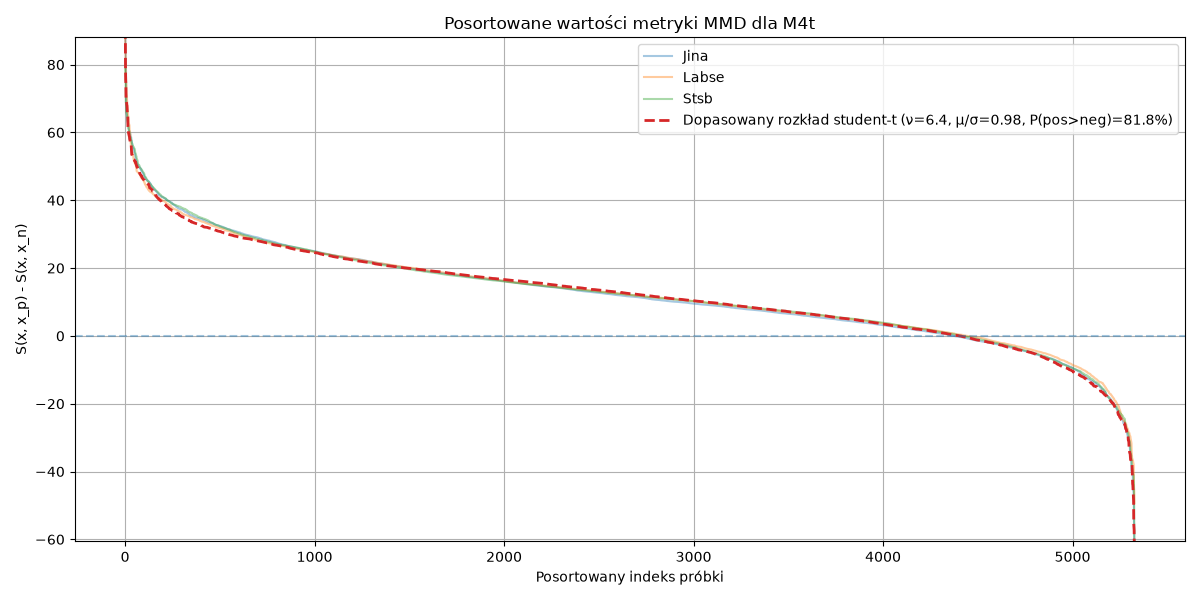
\includegraphics[width=0.8\linewidth]{figures/semantics/m4t_hani.png}
    \caption{Rozkład wartości różnicy podobieństw dla M4T w ramach zbioru \textit{Medical Speech, Transcription, and Intent}}
    \label{fig:latent:medicalM4T}
\end{figure}

\begin{figure}
    \centering
    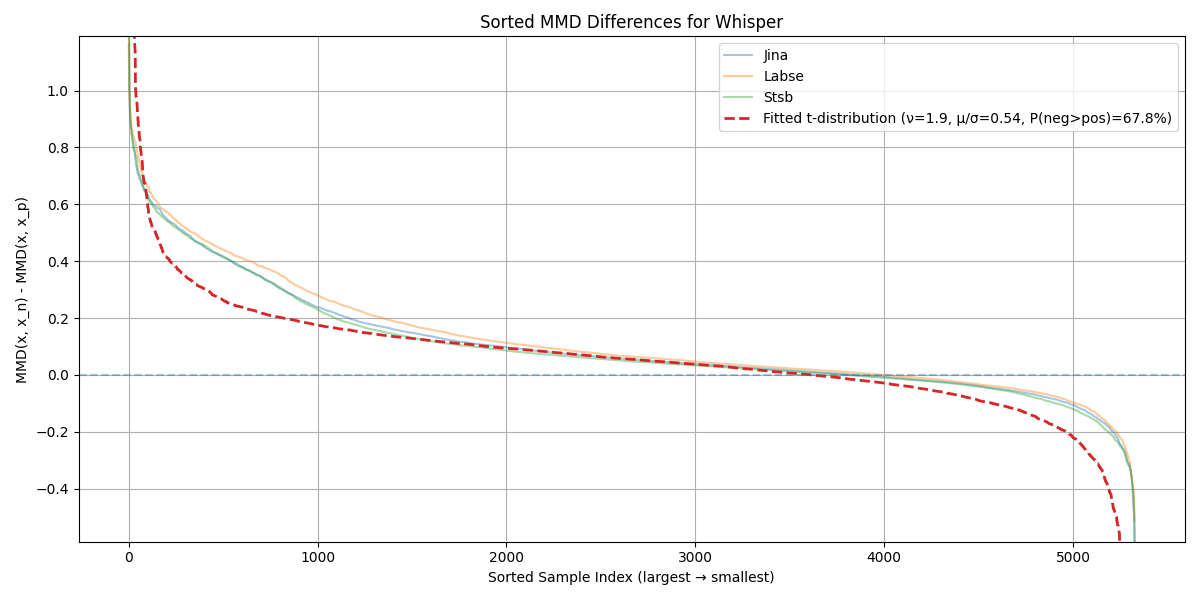
\includegraphics[width=0.8\linewidth]{figures/semantics/whisper.png}
    \caption{Rozkład wartości różnicy podobieństw dla Whisper w ramach zbioru \textit{Medical Speech, Transcription, and Intent}}
    \label{fig:latent:medicalWhisper}
\end{figure}

\begin{figure}
    \centering
    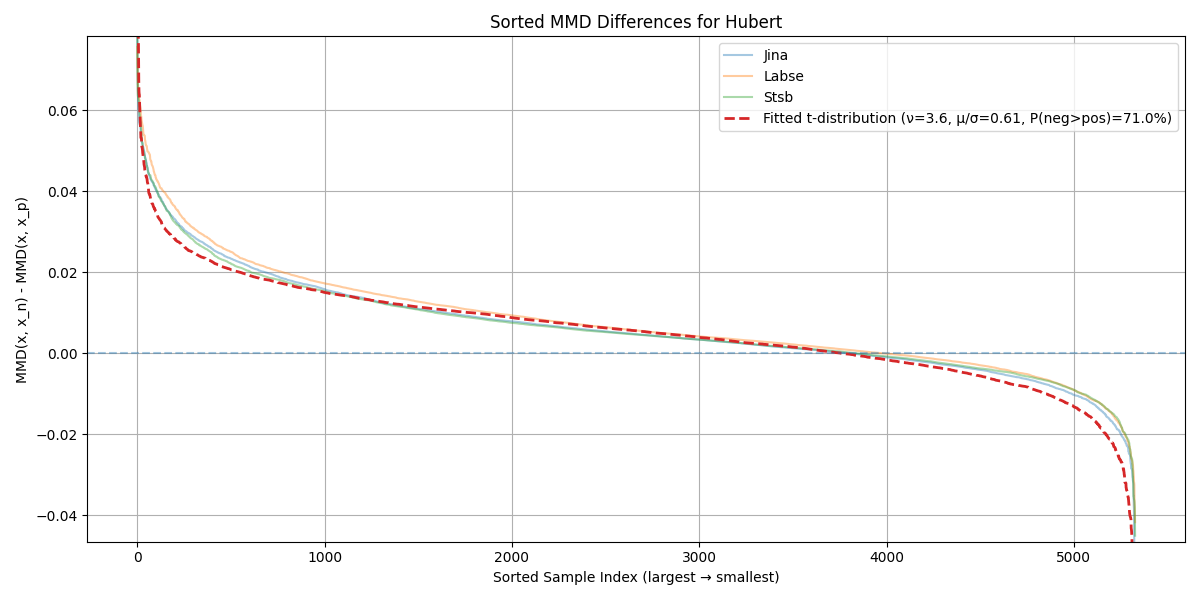
\includegraphics[width=0.8\linewidth]{figures/semantics/hubert.png}
    \caption{Rozkład wartości różnicy podobieństw dla Hubert w ramach zbioru \textit{Medical Speech, Transcription, and Intent}}
    \label{fig:latent:medicalHubert}
\end{figure}

\begin{figure}
    \centering
    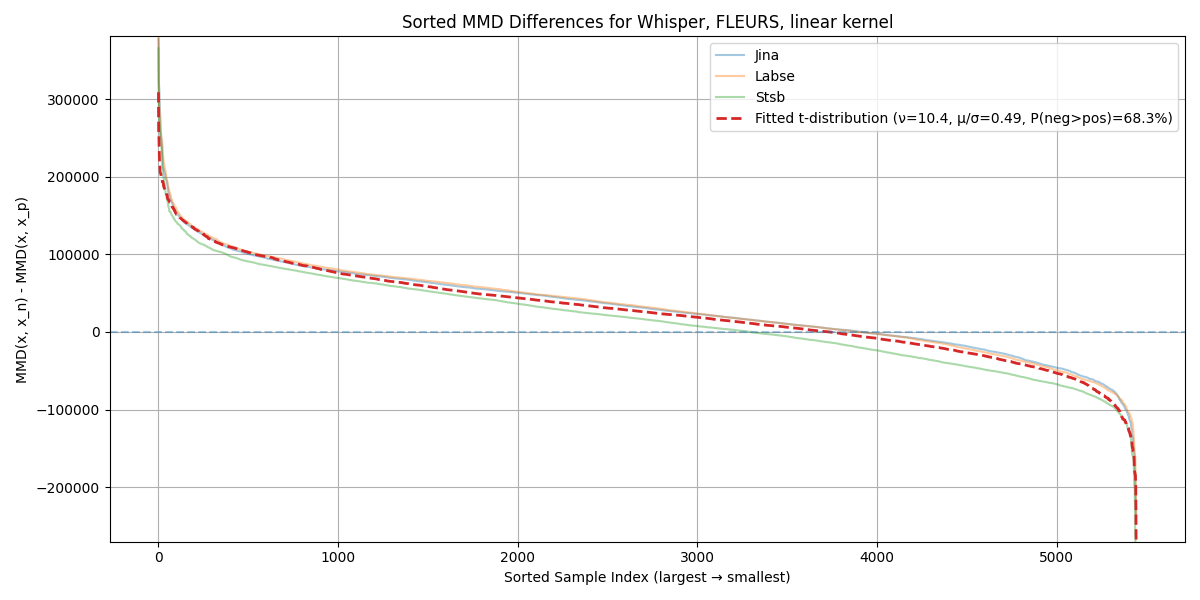
\includegraphics[width=0.8\linewidth]{figures/semantics/whisper_fleurs_linear.png}
    \caption{Rozkład wartości różnicy podobieństw dla Whisper w ramach zbioru \textit{Fleurs}}
    \label{fig:latent:fleursWhisper}
\end{figure}

\begin{figure}
    \centering
    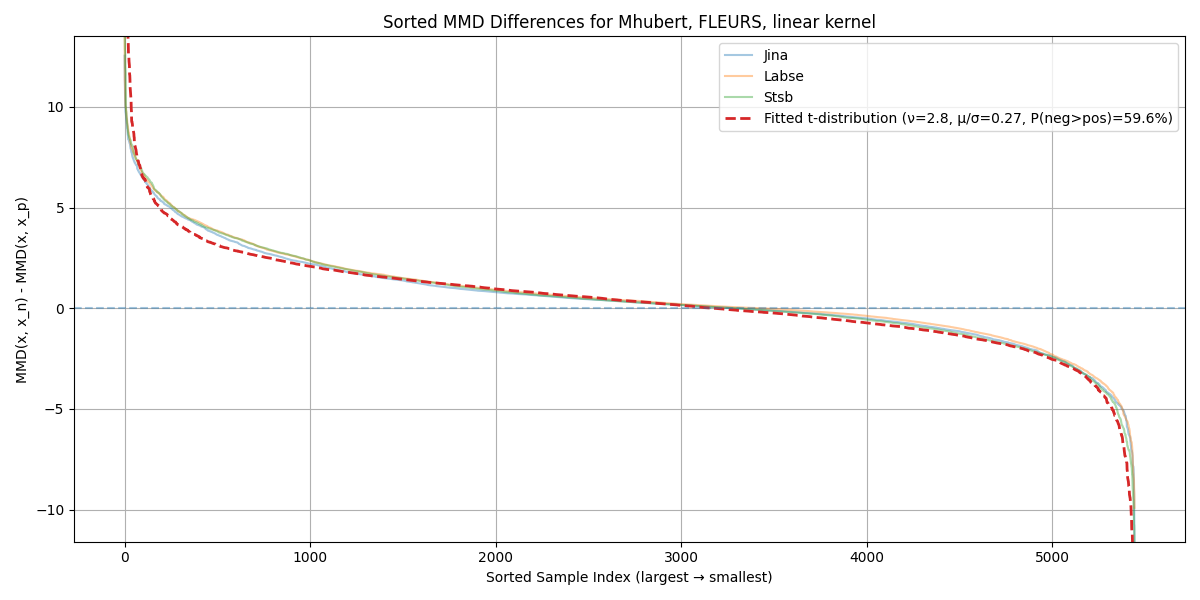
\includegraphics[width=0.8\linewidth]{figures/semantics/mhubert_fleurs_linear.png}
    \caption{Rozkład wartości różnicy podobieństw dla mHuBERT w ramach zbioru \textit{Fleurs}}
    \label{fig:latent:fleursMHubert}
\end{figure}

\begin{figure}
    \centering
    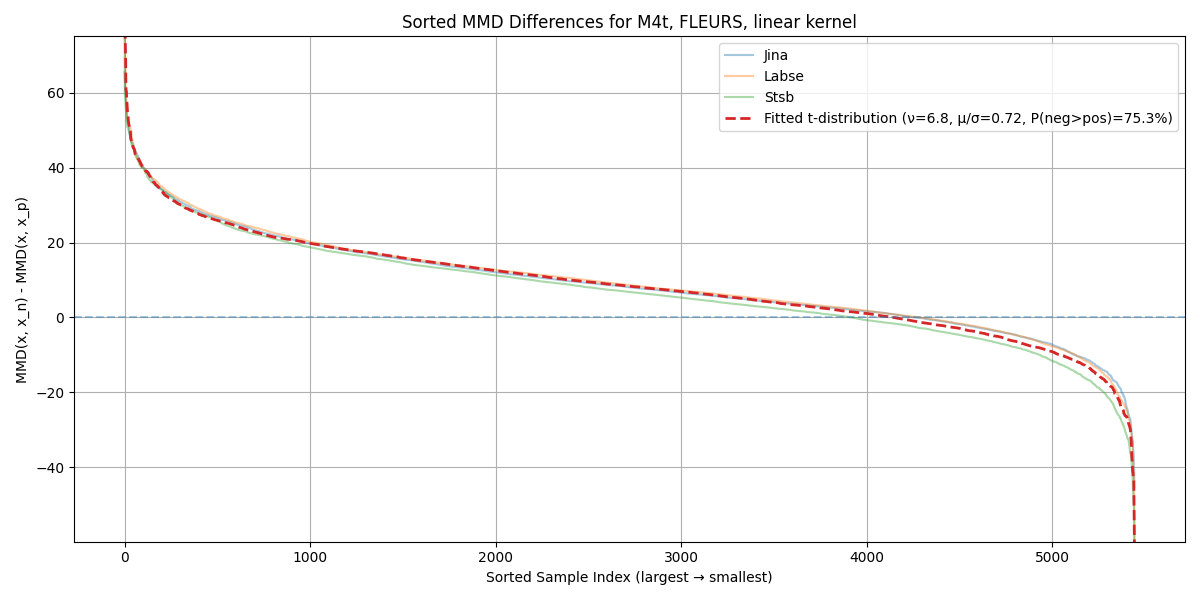
\includegraphics[width=0.8\linewidth]{figures/semantics/m4t_fleurs_linear.png}
    \caption{Rozkład wartości różnicy podobieństw dla M4T w ramach zbioru \textit{Fleurs}}
    \label{fig:latent:fleursM4T}
\end{figure}

\begin{figure}
    \centering
    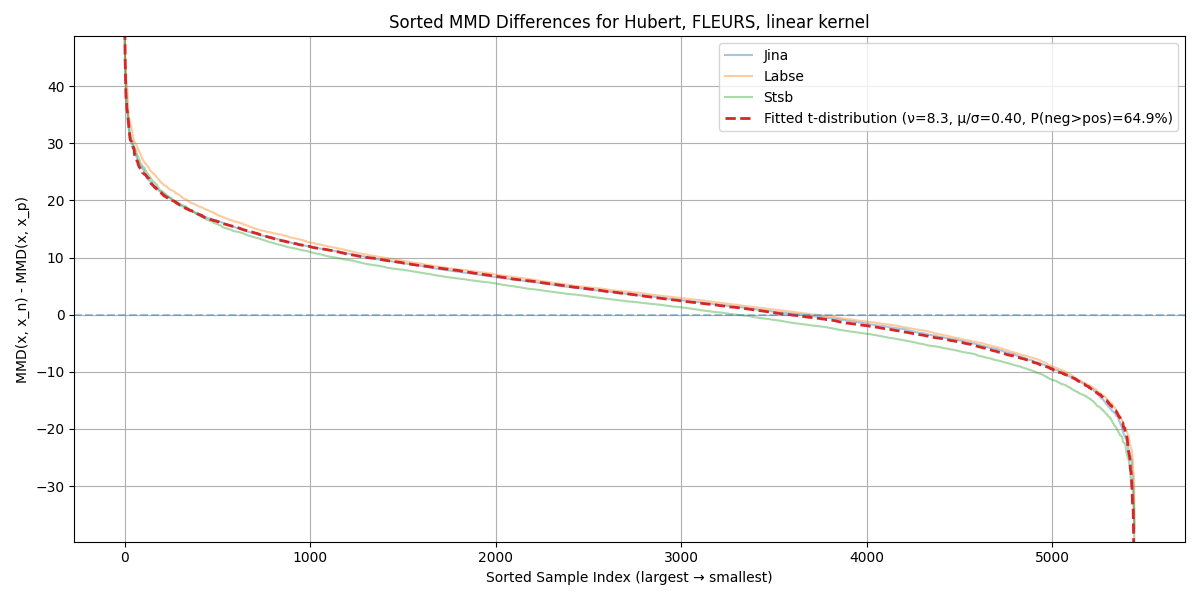
\includegraphics[width=0.8\linewidth]{figures/semantics/hubert_fleurs_linear.png}
    \caption{Rozkład wartości różnicy podobieństw dla HuBERT w ramach zbioru \textit{Fleurs}}
    \label{fig:latent:fleursHubert}
\end{figure}

\FloatBarrier


\subsection*{Analiza wpływu przetwarzania embeddingów na zachowanie semantyki}

\begin{figure}[!htbp]
    \centering
    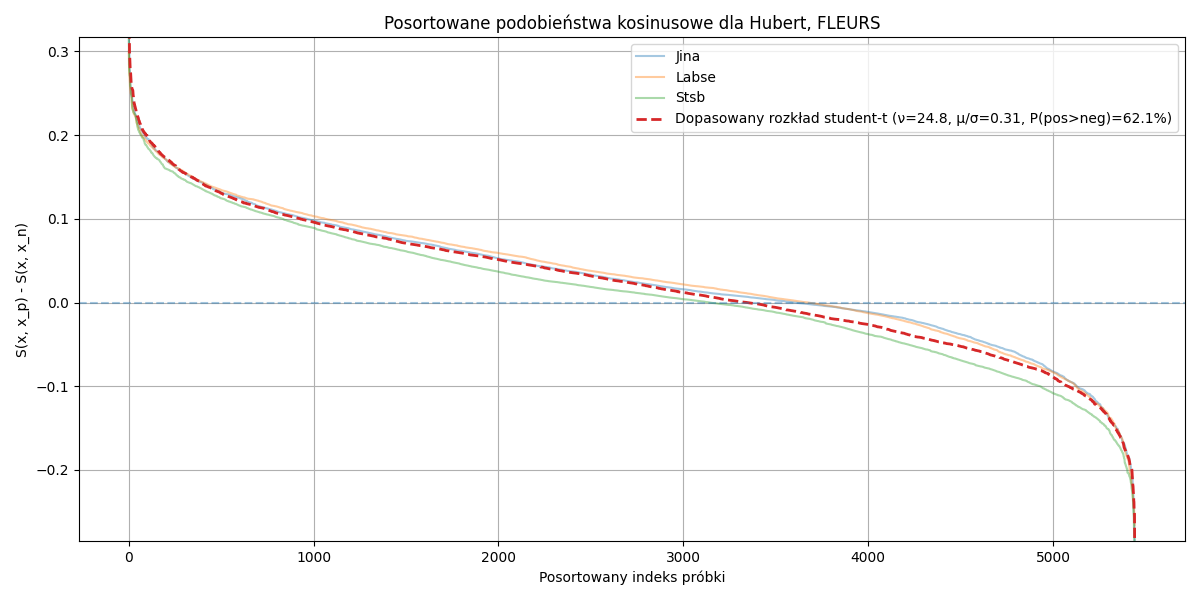
\includegraphics[width=0.8\linewidth]{figures/semantics/hubert_fleurs_linear_cosine.png}
    \caption{Rozkład wartości różnicy podobieństw dla HuBERT w ramach zbioru \textit{Fleurs}, \textit{mean pooling}}
    \label{fig:latent:simHubert}
\end{figure}

\begin{figure}[!htbp]
    \centering
    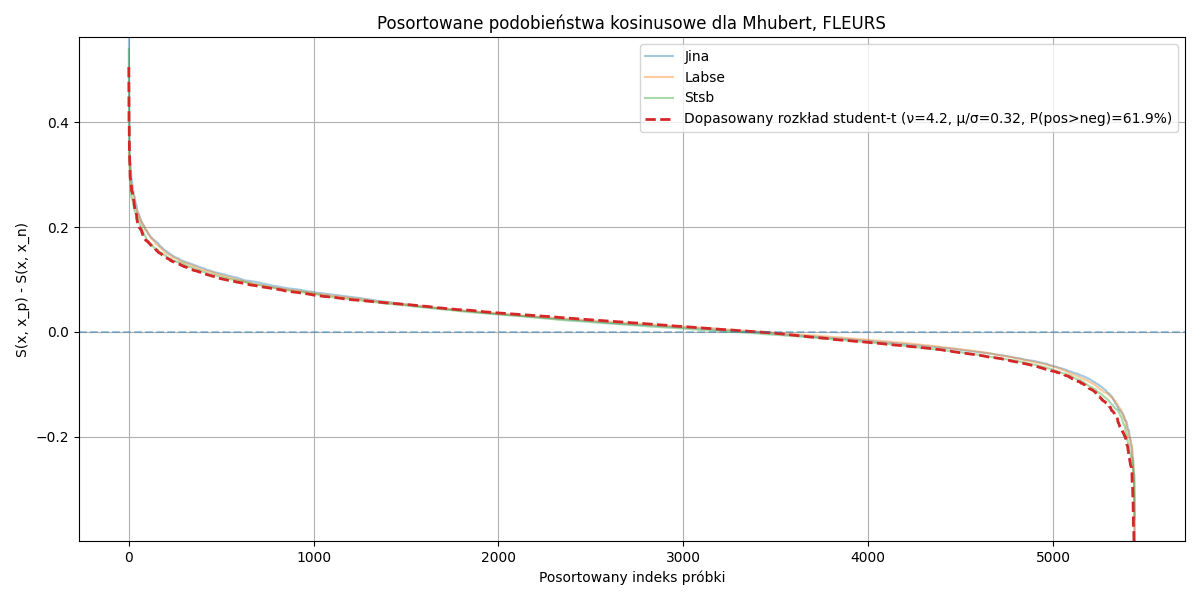
\includegraphics[width=0.8\linewidth]{figures/semantics/mhubert_fleurs_linear_cosine.png}
    \caption{Rozkład wartości różnicy podobieństw dla mHuBERT w ramach zbioru \textit{Fleurs}, \textit{mean pooling}}
    \label{fig:latent:simMhubert}
\end{figure}

\begin{figure}[!htbp]
    \centering
    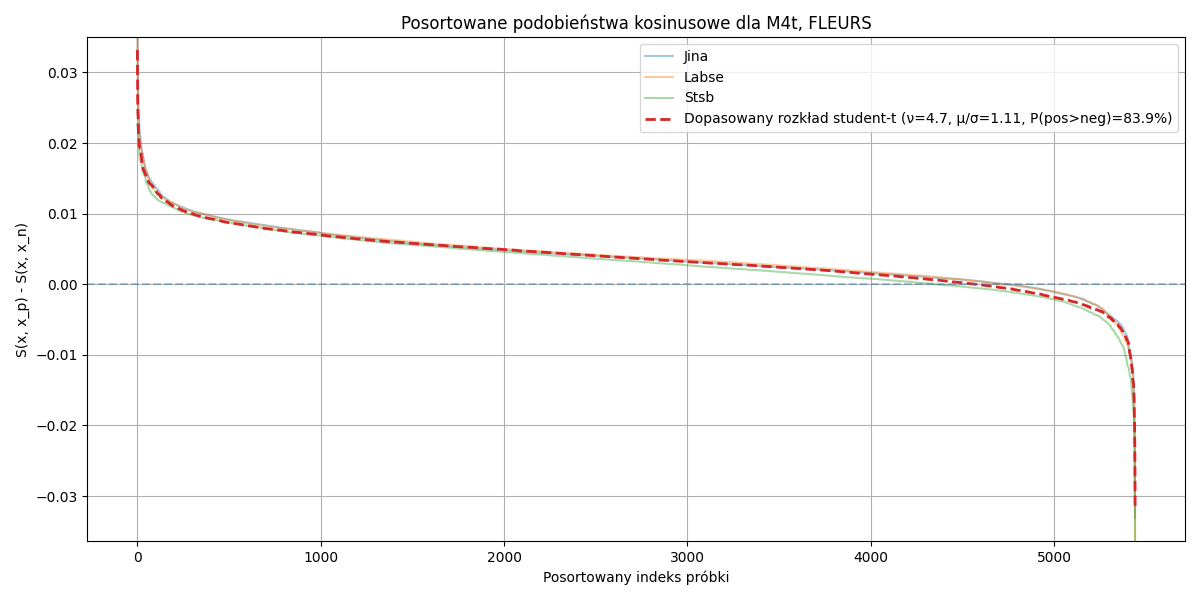
\includegraphics[width=0.8\linewidth]{figures/semantics/m4t_fleurs_linear_cosine.png}
    \caption{Rozkład wartości różnicy podobieństw dla SeamlessM4T w ramach zbioru \textit{Fleurs}, \textit{mean pooling}}
    \label{fig:latent:simM4T}
\end{figure}

\begin{figure}
    \centering
    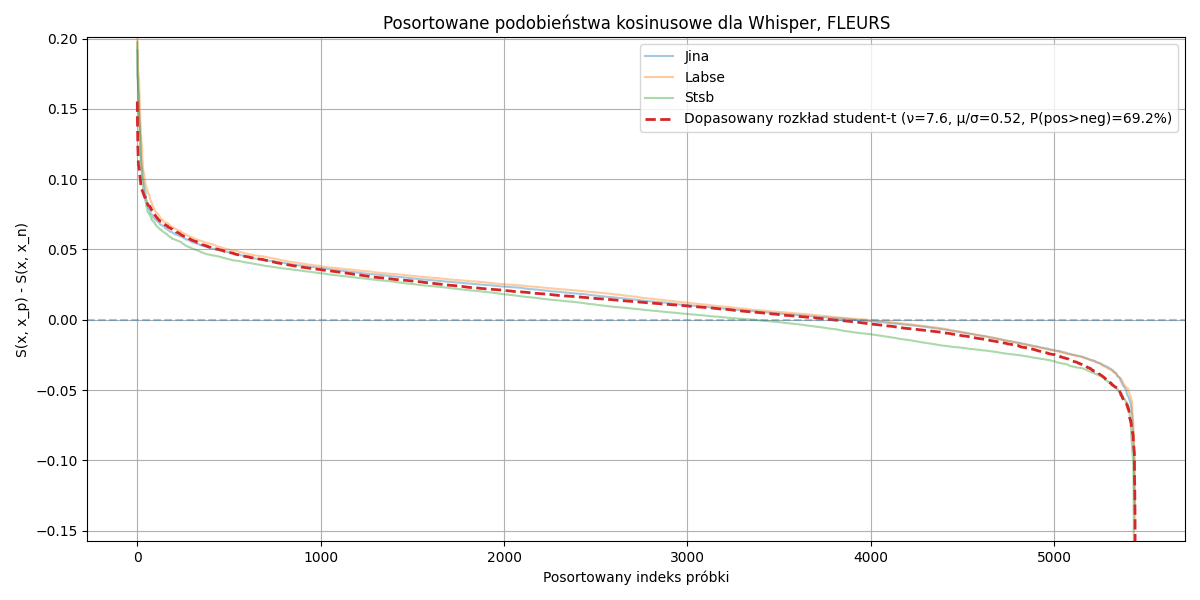
\includegraphics[width=0.8\linewidth]{figures/semantics/whisper_fleurs_linear_cosine.png}
    \caption{Rozkład wartości różnicy podobieństw dla Whisper w ramach zbioru \textit{Fleurs}, \textit{mean pooling}}
    \label{fig:latent:simWhisper}
\end{figure}


\begin{figure}
    \centering
    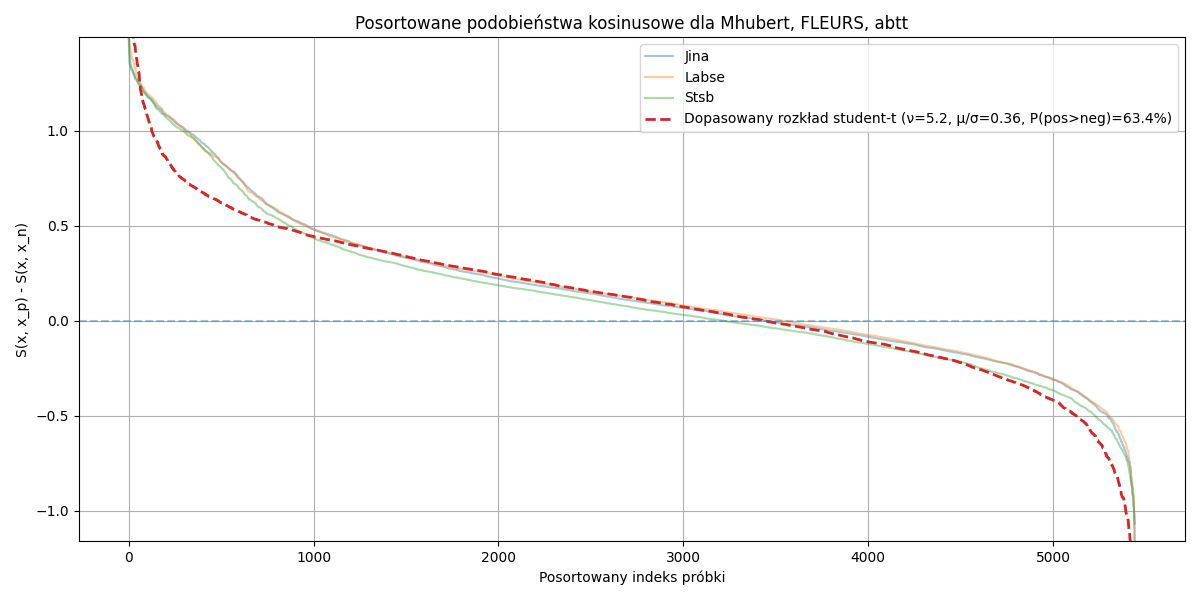
\includegraphics[width=0.8\linewidth]{figures/semantics/mhubert_fleurs_linear_abtt.png}
    \caption{Rozkład wartości różnicy podobieństw dla mHuBERT w ramach zbioru \textit{Fleurs}, \textit{mean pooling}, ABTT}
    \label{fig:latent:simMHubertAbtt}
\end{figure}

\begin{figure}
    \centering
    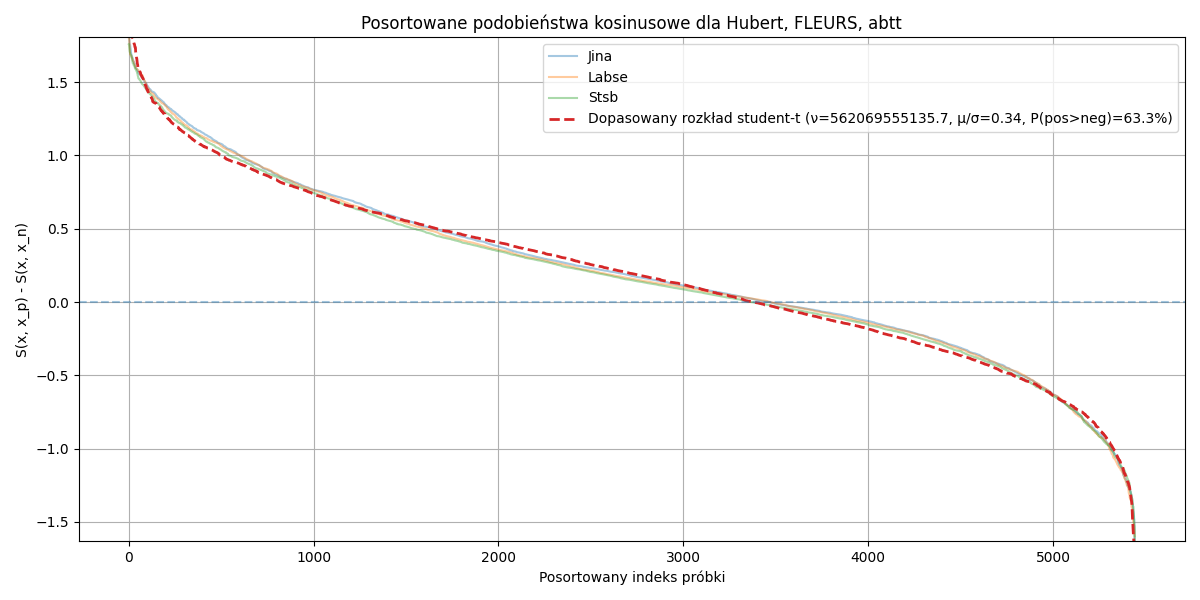
\includegraphics[width=0.8\linewidth]{figures/semantics/hubert_fleurs_linear_abtt.png}
    \caption{Rozkład wartości różnicy podobieństw dla HuBERT w ramach zbioru \textit{Fleurs}, \textit{mean pooling}, ABTT}
    \label{fig:latent:simHubertAbtt}
\end{figure}

\begin{figure}
    \centering
    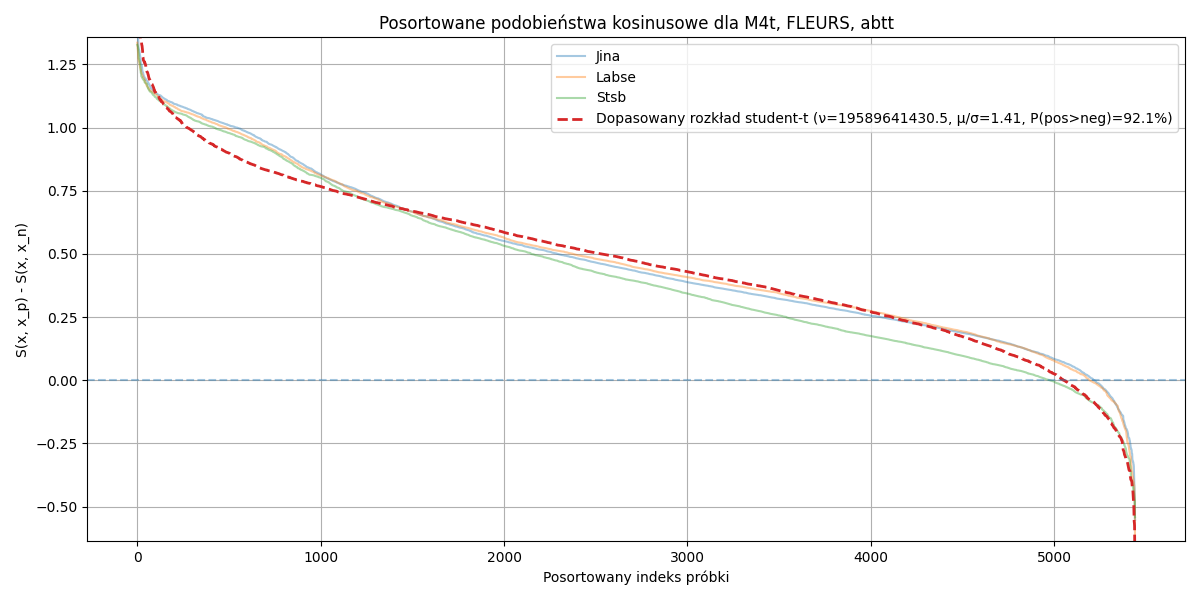
\includegraphics[width=0.8\linewidth]{figures/semantics/m4t_fleurs_linear_abtt.png}
    \caption{Rozkład wartości różnicy podobieństw dla SeamlessM4T w ramach zbioru \textit{Fleurs}, \textit{mean pooling}, ABTT}
    \label{fig:latent:simM4TAbtt}
\end{figure}

\begin{figure}
    \centering
    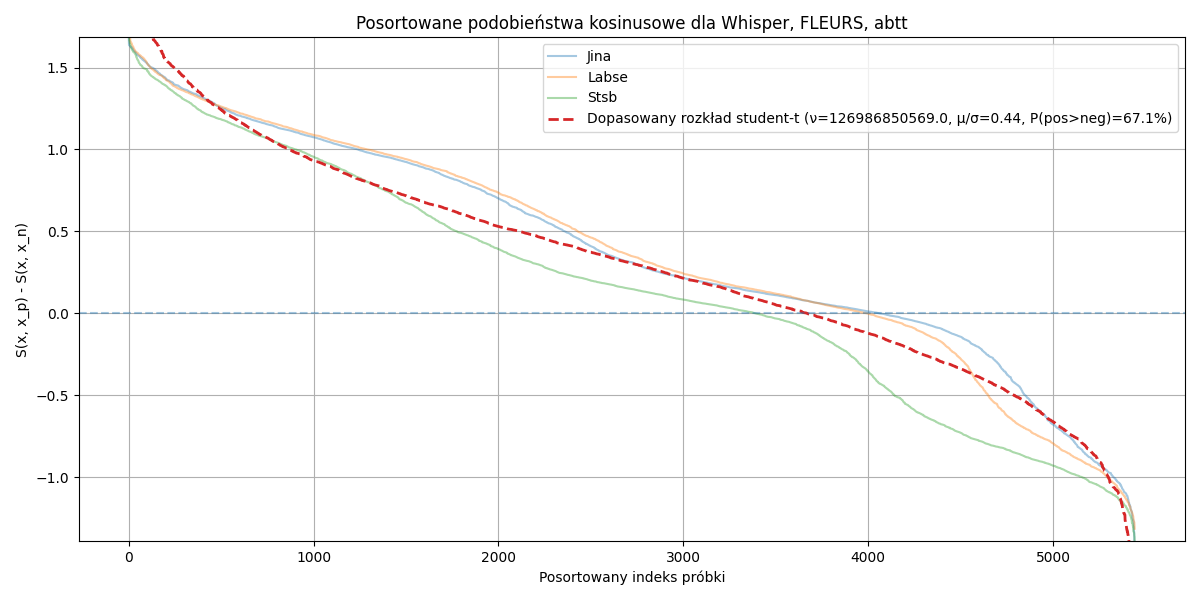
\includegraphics[width=0.8\linewidth]{figures/semantics/whisper_fleurs_linear_abtt.png}
    \caption{Rozkład wartości różnicy podobieństw dla Whisper w ramach zbioru \textit{Fleurs}, \textit{mean pooling}, ABTT}
    \label{fig:latent:simWhisperAbtt}
\end{figure}



\end{document}
